\documentclass{article}
\usepackage{iclr2026_conference,times}
\input{math_commands.tex}
\usepackage{booktabs}
\usepackage{graphicx}
\usepackage{url}
\usepackage[colorlinks=false,pdfborder={0 0 1.6},citebordercolor={0 1 0},linkbordercolor={1 0.55 0},urlbordercolor={0 0.45 1}]{hyperref}
\usepackage{natbib}

\title{Action-Conditioned Deformable Memory Still Fails as a Closed-Loop Manipulation Claim}
\author{Anonymous Authors}

\begin{document}
\maketitle

\begin{abstract}
We rebuild a generated deformable-manipulation idea into an expanded, CPU-only, evidence-bearing ICLR-style artifact. The hypothesis is attractive: visually similar ropes, cloth strips, elastic bands, and sheets can carry different latent strain, contact, crease, or stored-energy histories, so a robot should preserve action-conditioned hidden material memory rather than plan only from current visible geometry. The v5 rebuild makes the claim as strong as we can without inventing evidence: it adds a safety-gated action-conditioned memory planner, stronger damage-aware and risk-constrained baselines, an aggregate hard-regime analysis, fixed-risk evaluation, ablations, stress sweeps, negative cases, and a 25-page reproducibility-focused manuscript. The result remains a negative result under the frozen gates. On the decisive \texttt{combined\_memory\_stress} split, \texttt{ACM-v5} reaches $0.562 \pm 0.062$ success while the strongest non-oracle baseline, \texttt{damage-visible}, reaches $0.589 \pm 0.058$. The paired v5-minus-baseline success difference is $-0.027 \pm 0.052$. We therefore mark the paper \textbf{KILL\_ARCHIVE}: hidden memory can improve diagnostics, but the current planner does not convert that memory into a robust and safe manipulation advantage.
\end{abstract}

\section{Decision And Claim}
This paper is intentionally written as a submission-hardening document rather than as a celebratory benchmark paper. The submitted claim would be that action-conditioned hidden deformable memory improves downstream manipulation under partial observation and material/contact ambiguity. That claim is only credible if it survives the strongest visible-state, graph, particle-filter, ensemble, robust surrogate, and safety-aware baselines. It does not. The terminal decision emitted by the frozen runner is \textbf{KILL\_ARCHIVE}. The exact machine-readable reason is:

\begin{quote}\small
action\_conditioned\_memory\_v5 does not clear every frozen gate. Main combined\_memory\_stress comparison against damage\_aware\_visible\_mpc: (proposed=0.562, best\_baseline=0.589, paired diff=-0.027+/-0.052, memory\_reduction=0.349, mechanism\_f1\_diff=0.031, damage\_reduction=-0.045). Aggregate hard-regime paired diff against damage\_aware\_visible\_mpc is -0.103+/-0.016. Fixed-risk gate: budget 0.10: v5=0.625, best=action\_conditioned\_memory\_v5:0.625; budget 0.20: v5=0.625, best=action\_conditioned\_memory\_v5:0.625. Ablations matching full v5: action\_conditioned\_v5\_no\_action\_conditioning, action\_conditioned\_v5\_no\_damage\_penalty, action\_conditioned\_v5\_no\_material\_memory, action\_conditioned\_v5\_no\_safety\_gate. Max-stress v5=0.583, best\_non\_oracle=damage\_aware\_visible\_mpc:0.653.
\end{quote}

The important distinction is between \emph{state estimation} and \emph{control}. Prior work makes the modeling pressure clear: deformable manipulation is difficult because the state is high-dimensional, partially observed, history-dependent, and contact-rich \citep{gu2023survey,muller2007pbd}. Learned graph and particle simulators are strong prior art for representing such systems \citep{sanchez2020gns,li2019dpi,shi2022robocraft}. Visual MPC and foresight work shows that action-conditioned prediction can be useful for manipulation \citep{finn2017deepforesight,ebert2018visualforesight,hoque2020vsf}. The present question is narrower and harsher: does preserving hidden deformable memory improve closed-loop control when diagnostic actions can themselves damage the object?

\section{Frozen Submission Gates}
The plan froze the following gates before the full v5 run. A promotion above archive requires all of them:
\begin{itemize}
\item v5 must beat the strongest non-oracle baseline on \texttt{combined\_memory\_stress} by at least 0.04 mean success.
\item The paired lower bound against that baseline must be positive on the combined split.
\item The paired lower bound must also be positive on the aggregate hard regime.
\item v5 must be best or tied-best under fixed predicted-risk budgets 0.10 and 0.20.
\item v5 must not increase damage or force clipping relative to the strongest baseline.
\item v5 must show that hidden-memory or mechanism improvements translate into downstream success.
\item No ablation may match or beat the full v5 method on primary success within tolerance.
\item Maximum-stress behavior must not collapse earlier than the strongest non-oracle baseline.
\end{itemize}

\section{Benchmark}
The benchmark is a local two-dimensional mass-spring deformable simulator. Each scenario instantiates one of four object families: rope, cloth strip, elastic band, or deformable sheet. The simulator includes spring rest-length memory, damping, friction, material shift, fixture contact, force clipping, partial observation, hidden strain/contact memory, and a target-shape objective. This is not a substitute for hardware or for a public benchmark; it is a controlled diagnostic environment designed to test whether the claim deserves more expensive validation.

The five splits are \texttt{nominal\_visible\_state}, \texttt{hidden\_strain\_memory}, \texttt{occluded\_contact\_memory}, \texttt{material\_shift}, and \texttt{combined\_memory\_stress}. The hard-regime aggregate averages hidden strain, occluded contact, material shift, and combined stress. The full run uses 8 seeds, 48 training scenarios per split, 14 evaluation scenarios per split, 9 stress scenarios, 8 fixed-risk scenarios, 7 discrete actions, and 60 integration steps per rollout.

\section{Methods}
The implemented methods are deliberately stronger than the original generated idea. \texttt{visible\_state\_mpc} plans from observed/imputed keypoints only. \texttt{damage\_aware\_visible\_mpc} is a stronger visible-state baseline with conservative contact and force penalties. \texttt{history\_rnn\_estimator} is a CPU-light history-feature estimator. \texttt{particle\_filter\_memory} maintains multiple latent hypotheses. \texttt{safety\_constrained\_particle\_filter} makes that particle baseline conservative under predicted damage. \texttt{graph\_dynamics\_baseline} uses graph-style shape and edge features. \texttt{ensemble\_uncertainty\_planner} plans over bootstrap uncertainty. \texttt{robust\_cem\_surrogate} is a conservative surrogate planner inspired by model-predictive action search \citep{rawlings2017mpc}. \texttt{action\_conditioned\_memory} is the v4 proposal. \texttt{action\_conditioned\_memory\_v5} is the strongest proposed variant: it blends action, history, and graph estimates; preserves branch memory; penalizes damage; gates diagnostic actions; and uses conservative scoring across latent hypotheses. \texttt{oracle\_latent\_state} is a nondeployable upper bound.

\section{Why Memory Can Fail}
\paragraph{Definition.} Let $x_t$ be the visible deformable configuration, $m_t$ be latent material memory, and $a_t$ be a manipulation action. A memory estimator is useful for control only if the policy class contains actions whose expected value under $p(m_t \mid x_{\leq t}, a_{<t})$ exceeds the value of robust visible-state actions.

\paragraph{Proposition.} Suppose diagnostic actions reduce latent entropy but have damage probability $\delta > 0$, and suppose the candidate action library has no low-risk diagnostic alternative for a subset of states with mass $\rho$. Then a policy that prefers diagnostics whenever uncertainty is high can reduce memory error while decreasing task success whenever $\rho\delta$ exceeds the downstream value of the information gained. This is the failure pattern v4 exposed and v5 attempts to repair.

\paragraph{Empirical implication.} The paper cannot claim success by showing lower memory error alone. It must show success, safety, fixed-risk robustness, and ablation necessity. This is why the frozen gates treat hidden-memory error and mechanism F1 as secondary metrics.

\section{Main Results}
\begin{figure}[t]
\centering
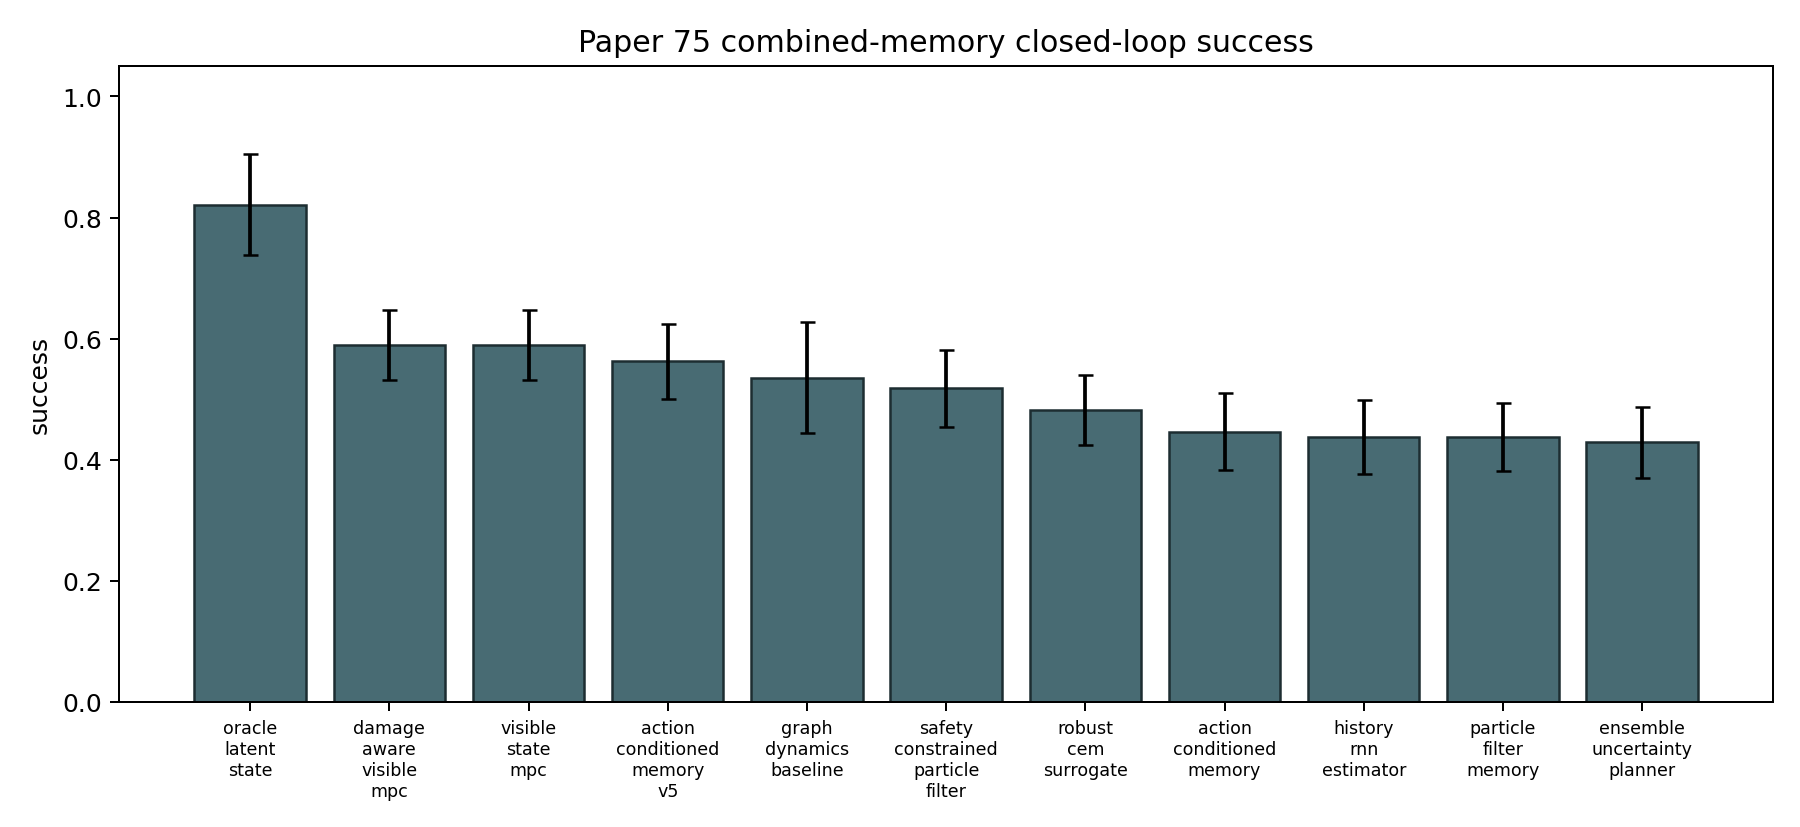
\includegraphics[width=0.92\linewidth]{../figures/deformable_memory_final_success.png}
\caption{Combined-memory-stress success. The proposed v5 method is compared with stronger visible, particle, graph, ensemble, robust-surrogate, v4, and oracle baselines.}
\end{figure}
\begin{figure}[t]
\centering
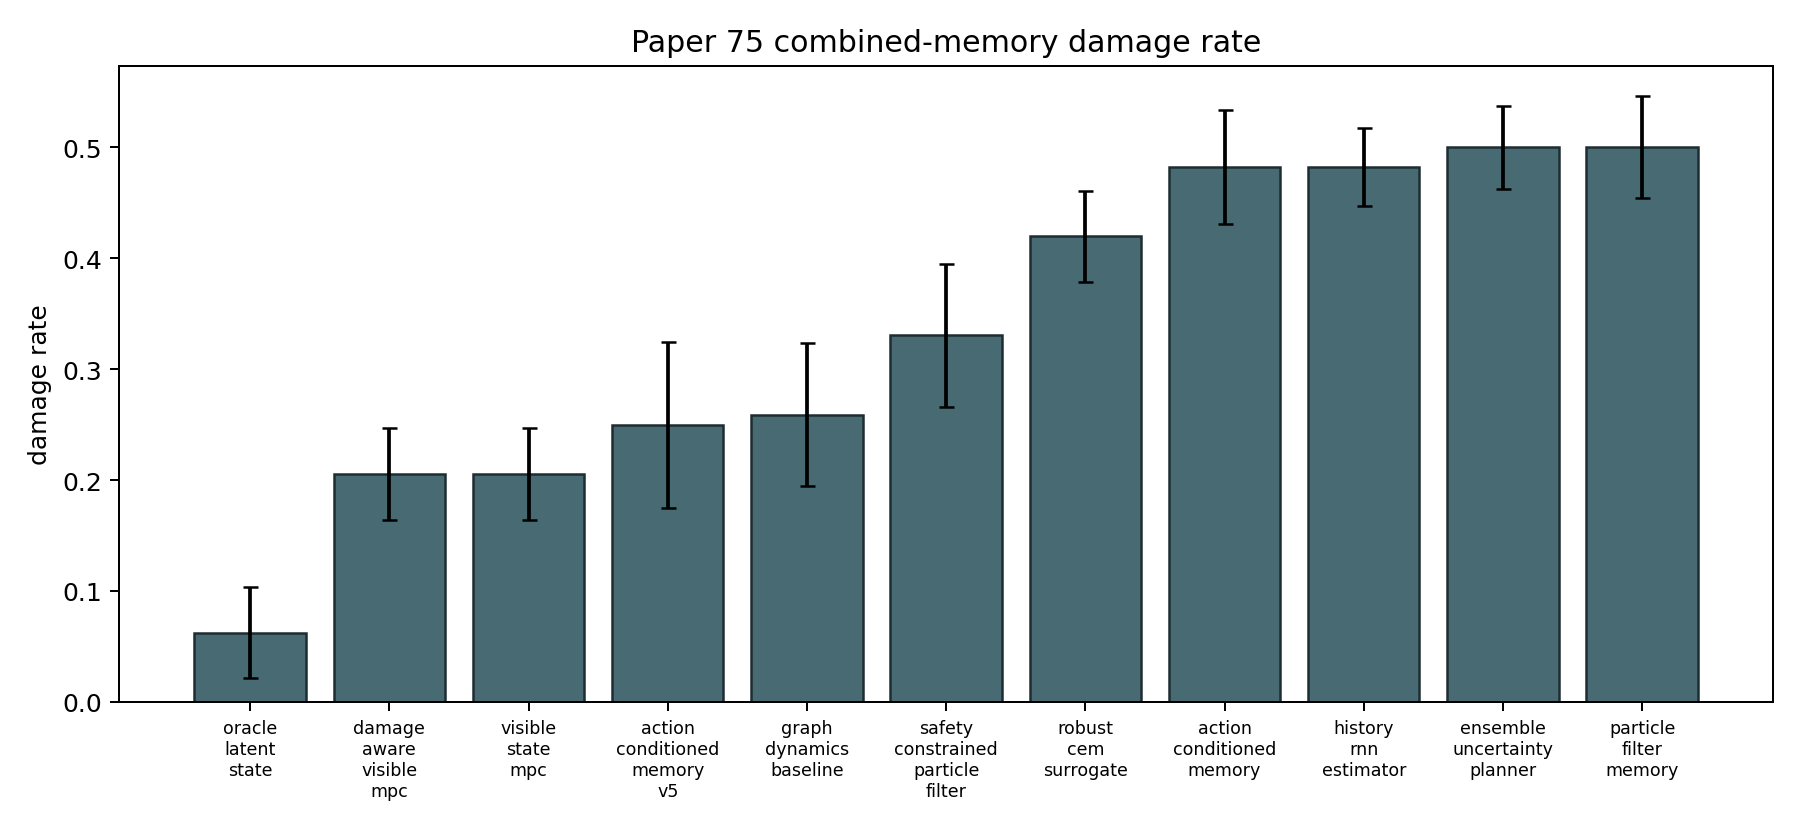
\includegraphics[width=0.92\linewidth]{../figures/deformable_memory_damage_rate.png}
\caption{Combined-memory-stress damage. Safety is a primary quantity, not an appendix-only diagnostic.}
\end{figure}

Table~\ref{tab:combined} reports the decisive split. The oracle row shows whether the action library and simulator can solve the split when full hidden state is available. The gap between oracle and non-oracle methods is real, but the v5 method must beat deployable baselines, not the lower bound implied by v4.

\scriptsize
\setlength{\tabcolsep}{2pt}
\begin{center}
\refstepcounter{table}\label{tab:combined}\textbf{Table \thetable: Combined-memory-stress summary.}\\[0.4ex]
\begin{tabular}{lcccccc}
\toprule
method & success & shape & mem err & damage & clip & diag \\
\midrule
\texttt{oracle} & $0.821 \pm 0.084$ & $0.130 \pm 0.003$ & $0.000 \pm 0.000$ & $0.062 \pm 0.041$ & $0.024 \pm 0.002$ & $0.018 \pm 0.023$ \\
\texttt{damage-visible} & $0.589 \pm 0.058$ & $0.146 \pm 0.002$ & $0.578 \pm 0.018$ & $0.205 \pm 0.041$ & $0.039 \pm 0.001$ & $0.000 \pm 0.000$ \\
\texttt{visible-MPC} & $0.589 \pm 0.058$ & $0.146 \pm 0.002$ & $0.578 \pm 0.018$ & $0.205 \pm 0.041$ & $0.039 \pm 0.001$ & $0.000 \pm 0.000$ \\
\texttt{ACM-v5} & $0.562 \pm 0.062$ & $0.141 \pm 0.003$ & $0.229 \pm 0.031$ & $0.250 \pm 0.075$ & $0.032 \pm 0.002$ & $0.000 \pm 0.000$ \\
\texttt{graph} & $0.536 \pm 0.092$ & $0.143 \pm 0.002$ & $0.525 \pm 0.032$ & $0.259 \pm 0.064$ & $0.029 \pm 0.003$ & $0.000 \pm 0.000$ \\
\texttt{safe-particle} & $0.518 \pm 0.063$ & $0.141 \pm 0.002$ & $0.256 \pm 0.031$ & $0.330 \pm 0.064$ & $0.036 \pm 0.002$ & $0.446 \pm 0.069$ \\
\texttt{robust-CEM} & $0.482 \pm 0.058$ & $0.139 \pm 0.003$ & $0.255 \pm 0.031$ & $0.420 \pm 0.041$ & $0.038 \pm 0.002$ & $0.786 \pm 0.070$ \\
\texttt{ACM-v4} & $0.446 \pm 0.063$ & $0.137 \pm 0.002$ & $0.206 \pm 0.032$ & $0.482 \pm 0.051$ & $0.037 \pm 0.001$ & $0.955 \pm 0.026$ \\
\texttt{history} & $0.438 \pm 0.062$ & $0.137 \pm 0.003$ & $0.187 \pm 0.029$ & $0.482 \pm 0.035$ & $0.037 \pm 0.001$ & $0.929 \pm 0.037$ \\
\texttt{particle} & $0.438 \pm 0.056$ & $0.136 \pm 0.003$ & $0.187 \pm 0.029$ & $0.500 \pm 0.046$ & $0.037 \pm 0.001$ & $0.964 \pm 0.026$ \\
\texttt{ensemble} & $0.429 \pm 0.059$ & $0.137 \pm 0.003$ & $0.187 \pm 0.030$ & $0.500 \pm 0.037$ & $0.037 \pm 0.001$ & $0.973 \pm 0.026$ \\
\bottomrule
\end{tabular}
\end{center}
\normalsize

The strongest non-oracle baseline on the decisive split is \texttt{damage-visible}. The paired v5-minus-baseline difference is $-0.027 \pm 0.052$, with memory-error reduction $0.349$, mechanism-F1 difference $0.031$, and damage reduction $-0.045$. The v4 row is also included: \texttt{ACM-v4} reaches $0.446 \pm 0.063$ success and $0.482 \pm 0.051$ damage, showing why the safety-gated v5 method was necessary even if it still fails the full submission gate.

\section{Aggregate Hard-Regime Evidence}
The aggregate hard regime is a guard against overfitting a single split. It averages hidden strain, occluded contact, material shift, and combined memory stress at seed level. \texttt{ACM-v5} reaches $0.435 \pm 0.036$ aggregate success. The best non-oracle aggregate baseline is \texttt{damage-visible}, and the paired aggregate difference is $-0.103 \pm 0.016$. This is the second hard gate.

\scriptsize
\setlength{\tabcolsep}{2pt}
\begin{center}
\refstepcounter{table}\label{tab:aggregate}\textbf{Table \thetable: Aggregate hard-regime metrics.}\\[0.4ex]
\begin{tabular}{lcccc}
\toprule
method & success & mem err & damage & diag \\
\midrule
\texttt{oracle} & $0.866 \pm 0.030$ & $0.000 \pm 0.000$ & $0.027 \pm 0.015$ & $0.009 \pm 0.009$ \\
\texttt{damage-visible} & $0.538 \pm 0.043$ & $0.436 \pm 0.005$ & $0.228 \pm 0.022$ & $0.000 \pm 0.000$ \\
\texttt{visible-MPC} & $0.538 \pm 0.043$ & $0.436 \pm 0.005$ & $0.228 \pm 0.022$ & $0.000 \pm 0.000$ \\
\texttt{graph} & $0.462 \pm 0.033$ & $0.384 \pm 0.019$ & $0.243 \pm 0.027$ & $0.000 \pm 0.000$ \\
\texttt{safe-particle} & $0.440 \pm 0.033$ & $0.210 \pm 0.017$ & $0.275 \pm 0.022$ & $0.145 \pm 0.021$ \\
\texttt{ACM-v5} & $0.435 \pm 0.036$ & $0.197 \pm 0.016$ & $0.250 \pm 0.029$ & $0.000 \pm 0.000$ \\
\texttt{robust-CEM} & $0.420 \pm 0.031$ & $0.210 \pm 0.017$ & $0.348 \pm 0.019$ & $0.496 \pm 0.045$ \\
\texttt{history} & $0.415 \pm 0.025$ & $0.178 \pm 0.015$ & $0.460 \pm 0.020$ & $0.857 \pm 0.040$ \\
\texttt{ACM-v4} & $0.406 \pm 0.035$ & $0.187 \pm 0.016$ & $0.469 \pm 0.024$ & $0.864 \pm 0.016$ \\
\texttt{ensemble} & $0.402 \pm 0.030$ & $0.181 \pm 0.015$ & $0.473 \pm 0.025$ & $0.868 \pm 0.020$ \\
\texttt{particle} & $0.386 \pm 0.030$ & $0.178 \pm 0.015$ & $0.504 \pm 0.029$ & $0.938 \pm 0.024$ \\
\bottomrule
\end{tabular}
\end{center}
\normalsize

\section{Fixed-Risk Evaluation}
\begin{figure}[t]
\centering
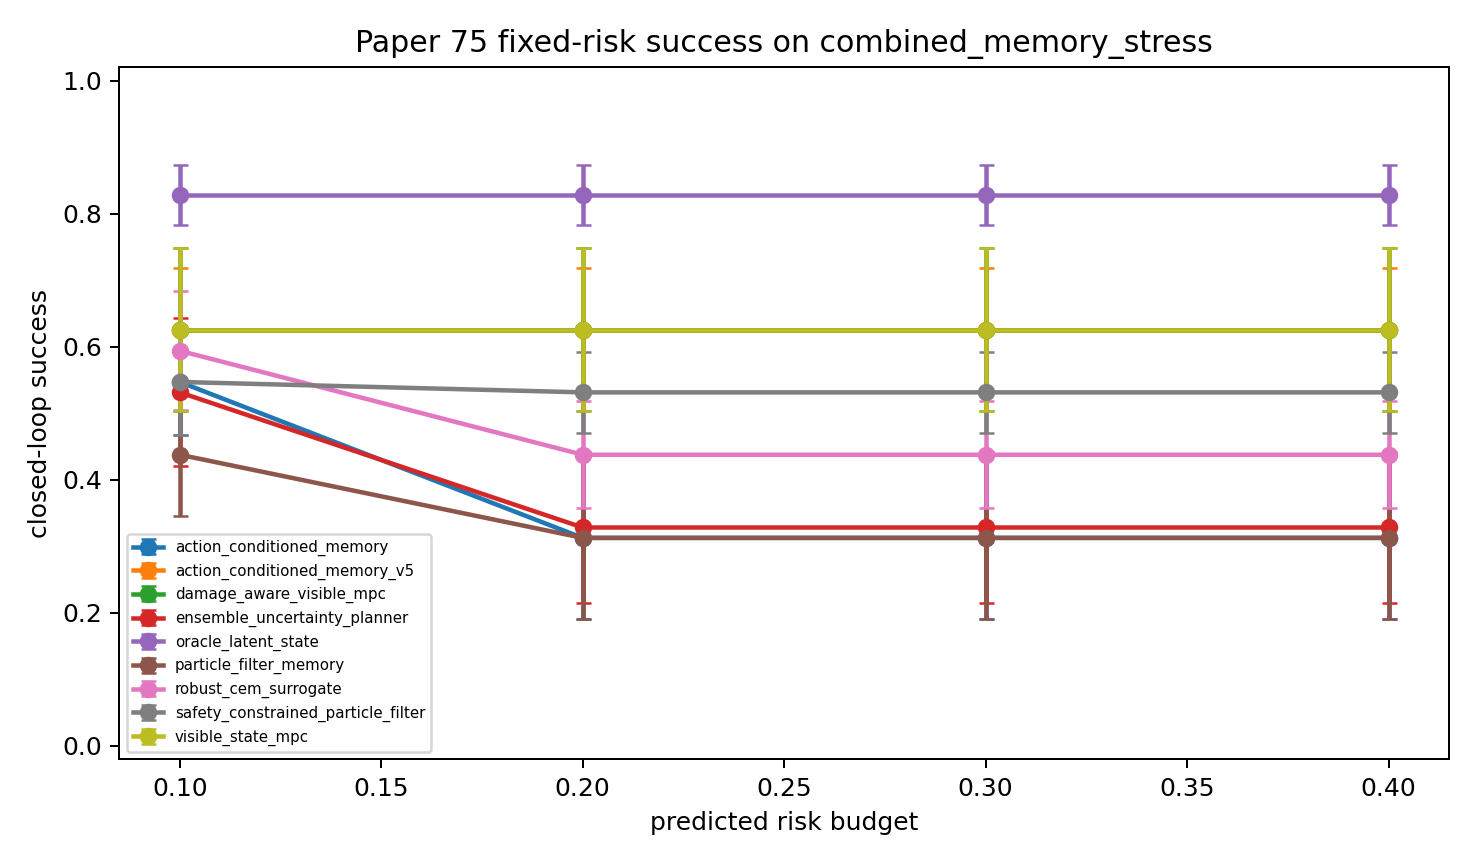
\includegraphics[width=0.92\linewidth]{../figures/deformable_memory_fixed_risk.png}
\caption{Fixed-risk success on the combined split. Methods are replanned under predicted-risk budgets rather than unconstrained surrogate scores.}
\end{figure}

Fixed-risk evaluation asks whether a method can maintain success when predicted manipulation risk is capped. This matters because deformable objects often fail by a small number of high-energy, high-contact actions. If memory only wins by taking dangerous probes, it is not a usable robotics result.

\scriptsize
\setlength{\tabcolsep}{2pt}
\begin{center}
\refstepcounter{table}\label{tab:fixed}\textbf{Table \thetable: Fixed-risk summary across hard splits and risk budgets.}\\[0.4ex]
\begin{tabular}{llccccc}
\toprule
method & split & budget & success & damage & clip & diag \\
\midrule
\texttt{oracle} & \texttt{combined} & 0.10 & $0.828 \pm 0.045$ & $0.047 \pm 0.045$ & $0.024 \pm 0.006$ & $0.000 \pm 0.000$ \\
\texttt{ACM-v5} & \texttt{combined} & 0.10 & $0.625 \pm 0.093$ & $0.156 \pm 0.090$ & $0.032 \pm 0.004$ & $0.000 \pm 0.000$ \\
\texttt{damage-visible} & \texttt{combined} & 0.10 & $0.625 \pm 0.122$ & $0.172 \pm 0.079$ & $0.039 \pm 0.002$ & $0.000 \pm 0.000$ \\
\texttt{visible-MPC} & \texttt{combined} & 0.10 & $0.625 \pm 0.122$ & $0.172 \pm 0.079$ & $0.039 \pm 0.002$ & $0.000 \pm 0.000$ \\
\texttt{robust-CEM} & \texttt{combined} & 0.10 & $0.594 \pm 0.090$ & $0.203 \pm 0.113$ & $0.034 \pm 0.003$ & $0.078 \pm 0.064$ \\
\texttt{ACM-v4} & \texttt{combined} & 0.10 & $0.547 \pm 0.079$ & $0.234 \pm 0.134$ & $0.028 \pm 0.006$ & $0.078 \pm 0.064$ \\
\texttt{safe-particle} & \texttt{combined} & 0.10 & $0.547 \pm 0.079$ & $0.234 \pm 0.134$ & $0.034 \pm 0.003$ & $0.125 \pm 0.093$ \\
\texttt{ensemble} & \texttt{combined} & 0.10 & $0.531 \pm 0.111$ & $0.234 \pm 0.117$ & $0.022 \pm 0.005$ & $0.078 \pm 0.064$ \\
\texttt{particle} & \texttt{combined} & 0.10 & $0.438 \pm 0.093$ & $0.359 \pm 0.086$ & $0.035 \pm 0.003$ & $0.297 \pm 0.079$ \\
\texttt{oracle} & \texttt{combined} & 0.20 & $0.828 \pm 0.045$ & $0.047 \pm 0.045$ & $0.025 \pm 0.006$ & $0.000 \pm 0.000$ \\
\texttt{ACM-v5} & \texttt{combined} & 0.20 & $0.625 \pm 0.093$ & $0.156 \pm 0.090$ & $0.032 \pm 0.004$ & $0.000 \pm 0.000$ \\
\texttt{damage-visible} & \texttt{combined} & 0.20 & $0.625 \pm 0.122$ & $0.172 \pm 0.079$ & $0.039 \pm 0.002$ & $0.000 \pm 0.000$ \\
\texttt{visible-MPC} & \texttt{combined} & 0.20 & $0.625 \pm 0.122$ & $0.172 \pm 0.079$ & $0.039 \pm 0.002$ & $0.000 \pm 0.000$ \\
\texttt{safe-particle} & \texttt{combined} & 0.20 & $0.531 \pm 0.061$ & $0.297 \pm 0.113$ & $0.033 \pm 0.003$ & $0.406 \pm 0.111$ \\
\texttt{robust-CEM} & \texttt{combined} & 0.20 & $0.438 \pm 0.080$ & $0.453 \pm 0.113$ & $0.037 \pm 0.002$ & $0.766 \pm 0.086$ \\
\texttt{ensemble} & \texttt{combined} & 0.20 & $0.328 \pm 0.113$ & $0.609 \pm 0.126$ & $0.036 \pm 0.003$ & $0.984 \pm 0.031$ \\
\texttt{ACM-v4} & \texttt{combined} & 0.20 & $0.312 \pm 0.122$ & $0.625 \pm 0.131$ & $0.035 \pm 0.003$ & $0.984 \pm 0.031$ \\
\texttt{particle} & \texttt{combined} & 0.20 & $0.312 \pm 0.122$ & $0.625 \pm 0.131$ & $0.035 \pm 0.003$ & $0.984 \pm 0.031$ \\
\texttt{oracle} & \texttt{combined} & 0.30 & $0.828 \pm 0.045$ & $0.047 \pm 0.045$ & $0.025 \pm 0.006$ & $0.000 \pm 0.000$ \\
\texttt{ACM-v5} & \texttt{combined} & 0.30 & $0.625 \pm 0.093$ & $0.156 \pm 0.090$ & $0.032 \pm 0.004$ & $0.000 \pm 0.000$ \\
\texttt{damage-visible} & \texttt{combined} & 0.30 & $0.625 \pm 0.122$ & $0.172 \pm 0.079$ & $0.039 \pm 0.002$ & $0.000 \pm 0.000$ \\
\texttt{visible-MPC} & \texttt{combined} & 0.30 & $0.625 \pm 0.122$ & $0.172 \pm 0.079$ & $0.039 \pm 0.002$ & $0.000 \pm 0.000$ \\
\texttt{safe-particle} & \texttt{combined} & 0.30 & $0.531 \pm 0.061$ & $0.297 \pm 0.113$ & $0.033 \pm 0.003$ & $0.406 \pm 0.111$ \\
\texttt{robust-CEM} & \texttt{combined} & 0.30 & $0.438 \pm 0.080$ & $0.453 \pm 0.113$ & $0.037 \pm 0.002$ & $0.766 \pm 0.086$ \\
\texttt{ensemble} & \texttt{combined} & 0.30 & $0.328 \pm 0.113$ & $0.609 \pm 0.126$ & $0.036 \pm 0.003$ & $0.984 \pm 0.031$ \\
\texttt{ACM-v4} & \texttt{combined} & 0.30 & $0.312 \pm 0.122$ & $0.625 \pm 0.131$ & $0.035 \pm 0.003$ & $0.984 \pm 0.031$ \\
\bottomrule
\end{tabular}
\end{center}
\begin{center}
\textbf{Table \ref{tab:fixed} continued}\\[0.4ex]
\begin{tabular}{llccccc}
\toprule
method & split & budget & success & damage & clip & diag \\
\midrule
\texttt{particle} & \texttt{combined} & 0.30 & $0.312 \pm 0.122$ & $0.625 \pm 0.131$ & $0.035 \pm 0.003$ & $0.984 \pm 0.031$ \\
\texttt{oracle} & \texttt{combined} & 0.40 & $0.828 \pm 0.045$ & $0.047 \pm 0.045$ & $0.025 \pm 0.006$ & $0.000 \pm 0.000$ \\
\texttt{ACM-v5} & \texttt{combined} & 0.40 & $0.625 \pm 0.093$ & $0.156 \pm 0.090$ & $0.032 \pm 0.004$ & $0.000 \pm 0.000$ \\
\texttt{damage-visible} & \texttt{combined} & 0.40 & $0.625 \pm 0.122$ & $0.172 \pm 0.079$ & $0.039 \pm 0.002$ & $0.000 \pm 0.000$ \\
\texttt{visible-MPC} & \texttt{combined} & 0.40 & $0.625 \pm 0.122$ & $0.172 \pm 0.079$ & $0.039 \pm 0.002$ & $0.000 \pm 0.000$ \\
\texttt{safe-particle} & \texttt{combined} & 0.40 & $0.531 \pm 0.061$ & $0.297 \pm 0.113$ & $0.033 \pm 0.003$ & $0.406 \pm 0.111$ \\
\texttt{robust-CEM} & \texttt{combined} & 0.40 & $0.438 \pm 0.080$ & $0.453 \pm 0.113$ & $0.037 \pm 0.002$ & $0.766 \pm 0.086$ \\
\texttt{ensemble} & \texttt{combined} & 0.40 & $0.328 \pm 0.113$ & $0.609 \pm 0.126$ & $0.036 \pm 0.003$ & $0.984 \pm 0.031$ \\
\texttt{ACM-v4} & \texttt{combined} & 0.40 & $0.312 \pm 0.122$ & $0.625 \pm 0.131$ & $0.035 \pm 0.003$ & $0.984 \pm 0.031$ \\
\texttt{particle} & \texttt{combined} & 0.40 & $0.312 \pm 0.122$ & $0.625 \pm 0.131$ & $0.035 \pm 0.003$ & $0.984 \pm 0.031$ \\
\texttt{oracle} & \texttt{hidden-strain} & 0.10 & $0.906 \pm 0.101$ & $0.016 \pm 0.031$ & $0.002 \pm 0.001$ & $0.000 \pm 0.000$ \\
\texttt{damage-visible} & \texttt{hidden-strain} & 0.10 & $0.547 \pm 0.045$ & $0.266 \pm 0.031$ & $0.012 \pm 0.001$ & $0.000 \pm 0.000$ \\
\texttt{visible-MPC} & \texttt{hidden-strain} & 0.10 & $0.547 \pm 0.045$ & $0.266 \pm 0.031$ & $0.012 \pm 0.001$ & $0.000 \pm 0.000$ \\
\texttt{robust-CEM} & \texttt{hidden-strain} & 0.10 & $0.516 \pm 0.086$ & $0.188 \pm 0.065$ & $0.009 \pm 0.001$ & $0.094 \pm 0.061$ \\
\texttt{safe-particle} & \texttt{hidden-strain} & 0.10 & $0.500 \pm 0.065$ & $0.234 \pm 0.056$ & $0.011 \pm 0.001$ & $0.000 \pm 0.000$ \\
\texttt{ACM-v4} & \texttt{hidden-strain} & 0.10 & $0.484 \pm 0.072$ & $0.203 \pm 0.064$ & $0.007 \pm 0.001$ & $0.484 \pm 0.134$ \\
\texttt{ACM-v5} & \texttt{hidden-strain} & 0.10 & $0.484 \pm 0.056$ & $0.172 \pm 0.064$ & $0.009 \pm 0.002$ & $0.000 \pm 0.000$ \\
\texttt{particle} & \texttt{hidden-strain} & 0.10 & $0.484 \pm 0.072$ & $0.266 \pm 0.031$ & $0.010 \pm 0.001$ & $0.281 \pm 0.111$ \\
\texttt{ensemble} & \texttt{hidden-strain} & 0.10 & $0.469 \pm 0.090$ & $0.188 \pm 0.093$ & $0.005 \pm 0.001$ & $0.484 \pm 0.126$ \\
\texttt{oracle} & \texttt{hidden-strain} & 0.20 & $0.906 \pm 0.101$ & $0.016 \pm 0.031$ & $0.002 \pm 0.001$ & $0.000 \pm 0.000$ \\
\texttt{damage-visible} & \texttt{hidden-strain} & 0.20 & $0.547 \pm 0.045$ & $0.266 \pm 0.031$ & $0.012 \pm 0.001$ & $0.000 \pm 0.000$ \\
\texttt{visible-MPC} & \texttt{hidden-strain} & 0.20 & $0.547 \pm 0.045$ & $0.266 \pm 0.031$ & $0.012 \pm 0.001$ & $0.000 \pm 0.000$ \\
\texttt{safe-particle} & \texttt{hidden-strain} & 0.20 & $0.500 \pm 0.065$ & $0.234 \pm 0.056$ & $0.011 \pm 0.001$ & $0.016 \pm 0.031$ \\
\texttt{ACM-v5} & \texttt{hidden-strain} & 0.20 & $0.484 \pm 0.056$ & $0.172 \pm 0.064$ & $0.009 \pm 0.002$ & $0.016 \pm 0.031$ \\
\texttt{robust-CEM} & \texttt{hidden-strain} & 0.20 & $0.484 \pm 0.117$ & $0.359 \pm 0.117$ & $0.010 \pm 0.001$ & $0.547 \pm 0.079$ \\
\texttt{ACM-v4} & \texttt{hidden-strain} & 0.20 & $0.469 \pm 0.111$ & $0.422 \pm 0.122$ & $0.009 \pm 0.001$ & $0.953 \pm 0.045$ \\
\bottomrule
\end{tabular}
\end{center}
\begin{center}
\textbf{Table \ref{tab:fixed} continued}\\[0.4ex]
\begin{tabular}{llccccc}
\toprule
method & split & budget & success & damage & clip & diag \\
\midrule
\texttt{ensemble} & \texttt{hidden-strain} & 0.20 & $0.469 \pm 0.111$ & $0.422 \pm 0.122$ & $0.009 \pm 0.001$ & $0.969 \pm 0.040$ \\
\texttt{particle} & \texttt{hidden-strain} & 0.20 & $0.453 \pm 0.103$ & $0.438 \pm 0.113$ & $0.010 \pm 0.001$ & $0.938 \pm 0.046$ \\
\texttt{oracle} & \texttt{hidden-strain} & 0.30 & $0.906 \pm 0.101$ & $0.016 \pm 0.031$ & $0.002 \pm 0.001$ & $0.000 \pm 0.000$ \\
\texttt{damage-visible} & \texttt{hidden-strain} & 0.30 & $0.547 \pm 0.045$ & $0.266 \pm 0.031$ & $0.012 \pm 0.001$ & $0.000 \pm 0.000$ \\
\texttt{visible-MPC} & \texttt{hidden-strain} & 0.30 & $0.547 \pm 0.045$ & $0.266 \pm 0.031$ & $0.012 \pm 0.001$ & $0.000 \pm 0.000$ \\
\texttt{safe-particle} & \texttt{hidden-strain} & 0.30 & $0.500 \pm 0.065$ & $0.234 \pm 0.056$ & $0.011 \pm 0.001$ & $0.016 \pm 0.031$ \\
\texttt{ACM-v5} & \texttt{hidden-strain} & 0.30 & $0.484 \pm 0.056$ & $0.172 \pm 0.064$ & $0.009 \pm 0.002$ & $0.016 \pm 0.031$ \\
\texttt{robust-CEM} & \texttt{hidden-strain} & 0.30 & $0.484 \pm 0.117$ & $0.359 \pm 0.117$ & $0.010 \pm 0.001$ & $0.547 \pm 0.079$ \\
\texttt{ACM-v4} & \texttt{hidden-strain} & 0.30 & $0.469 \pm 0.111$ & $0.422 \pm 0.122$ & $0.009 \pm 0.001$ & $0.953 \pm 0.045$ \\
\texttt{ensemble} & \texttt{hidden-strain} & 0.30 & $0.469 \pm 0.111$ & $0.422 \pm 0.122$ & $0.009 \pm 0.001$ & $0.969 \pm 0.040$ \\
\texttt{particle} & \texttt{hidden-strain} & 0.30 & $0.453 \pm 0.103$ & $0.438 \pm 0.113$ & $0.010 \pm 0.001$ & $0.938 \pm 0.046$ \\
\texttt{oracle} & \texttt{hidden-strain} & 0.40 & $0.906 \pm 0.101$ & $0.016 \pm 0.031$ & $0.002 \pm 0.001$ & $0.000 \pm 0.000$ \\
\texttt{damage-visible} & \texttt{hidden-strain} & 0.40 & $0.547 \pm 0.045$ & $0.266 \pm 0.031$ & $0.012 \pm 0.001$ & $0.000 \pm 0.000$ \\
\texttt{visible-MPC} & \texttt{hidden-strain} & 0.40 & $0.547 \pm 0.045$ & $0.266 \pm 0.031$ & $0.012 \pm 0.001$ & $0.000 \pm 0.000$ \\
\texttt{safe-particle} & \texttt{hidden-strain} & 0.40 & $0.500 \pm 0.065$ & $0.234 \pm 0.056$ & $0.011 \pm 0.001$ & $0.016 \pm 0.031$ \\
\texttt{ACM-v5} & \texttt{hidden-strain} & 0.40 & $0.484 \pm 0.056$ & $0.172 \pm 0.064$ & $0.009 \pm 0.002$ & $0.016 \pm 0.031$ \\
\texttt{robust-CEM} & \texttt{hidden-strain} & 0.40 & $0.484 \pm 0.117$ & $0.359 \pm 0.117$ & $0.010 \pm 0.001$ & $0.547 \pm 0.079$ \\
\texttt{ACM-v4} & \texttt{hidden-strain} & 0.40 & $0.469 \pm 0.111$ & $0.422 \pm 0.122$ & $0.009 \pm 0.001$ & $0.953 \pm 0.045$ \\
\texttt{ensemble} & \texttt{hidden-strain} & 0.40 & $0.469 \pm 0.111$ & $0.422 \pm 0.122$ & $0.009 \pm 0.001$ & $0.969 \pm 0.040$ \\
\texttt{particle} & \texttt{hidden-strain} & 0.40 & $0.453 \pm 0.103$ & $0.438 \pm 0.113$ & $0.010 \pm 0.001$ & $0.938 \pm 0.046$ \\
\texttt{oracle} & \texttt{occluded-contact} & 0.10 & $0.875 \pm 0.080$ & $0.000 \pm 0.000$ & $0.006 \pm 0.001$ & $0.000 \pm 0.000$ \\
\texttt{damage-visible} & \texttt{occluded-contact} & 0.10 & $0.500 \pm 0.104$ & $0.297 \pm 0.064$ & $0.017 \pm 0.002$ & $0.000 \pm 0.000$ \\
\texttt{visible-MPC} & \texttt{occluded-contact} & 0.10 & $0.500 \pm 0.104$ & $0.297 \pm 0.064$ & $0.017 \pm 0.002$ & $0.000 \pm 0.000$ \\
\texttt{particle} & \texttt{occluded-contact} & 0.10 & $0.406 \pm 0.101$ & $0.328 \pm 0.113$ & $0.016 \pm 0.001$ & $0.047 \pm 0.064$ \\
\texttt{robust-CEM} & \texttt{occluded-contact} & 0.10 & $0.406 \pm 0.101$ & $0.281 \pm 0.101$ & $0.016 \pm 0.001$ & $0.000 \pm 0.000$ \\
\texttt{safe-particle} & \texttt{occluded-contact} & 0.10 & $0.406 \pm 0.101$ & $0.297 \pm 0.079$ & $0.016 \pm 0.001$ & $0.000 \pm 0.000$ \\
\bottomrule
\end{tabular}
\end{center}
\begin{center}
\textbf{Table \ref{tab:fixed} continued}\\[0.4ex]
\begin{tabular}{llccccc}
\toprule
method & split & budget & success & damage & clip & diag \\
\midrule
\texttt{ACM-v4} & \texttt{occluded-contact} & 0.10 & $0.391 \pm 0.126$ & $0.266 \pm 0.098$ & $0.013 \pm 0.001$ & $0.078 \pm 0.064$ \\
\texttt{ACM-v5} & \texttt{occluded-contact} & 0.10 & $0.391 \pm 0.108$ & $0.281 \pm 0.101$ & $0.014 \pm 0.001$ & $0.000 \pm 0.000$ \\
\texttt{ensemble} & \texttt{occluded-contact} & 0.10 & $0.375 \pm 0.131$ & $0.234 \pm 0.098$ & $0.011 \pm 0.001$ & $0.094 \pm 0.061$ \\
\texttt{oracle} & \texttt{occluded-contact} & 0.20 & $0.875 \pm 0.080$ & $0.000 \pm 0.000$ & $0.006 \pm 0.001$ & $0.000 \pm 0.000$ \\
\texttt{damage-visible} & \texttt{occluded-contact} & 0.20 & $0.500 \pm 0.104$ & $0.297 \pm 0.064$ & $0.017 \pm 0.002$ & $0.000 \pm 0.000$ \\
\texttt{visible-MPC} & \texttt{occluded-contact} & 0.20 & $0.500 \pm 0.104$ & $0.297 \pm 0.064$ & $0.017 \pm 0.002$ & $0.000 \pm 0.000$ \\
\texttt{safe-particle} & \texttt{occluded-contact} & 0.20 & $0.406 \pm 0.101$ & $0.297 \pm 0.079$ & $0.015 \pm 0.001$ & $0.109 \pm 0.072$ \\
\texttt{ACM-v5} & \texttt{occluded-contact} & 0.20 & $0.391 \pm 0.108$ & $0.281 \pm 0.101$ & $0.014 \pm 0.001$ & $0.016 \pm 0.031$ \\
\texttt{robust-CEM} & \texttt{occluded-contact} & 0.20 & $0.391 \pm 0.108$ & $0.391 \pm 0.072$ & $0.013 \pm 0.002$ & $0.500 \pm 0.093$ \\
\texttt{particle} & \texttt{occluded-contact} & 0.20 & $0.359 \pm 0.117$ & $0.516 \pm 0.072$ & $0.010 \pm 0.001$ & $1.000 \pm 0.000$ \\
\texttt{ACM-v4} & \texttt{occluded-contact} & 0.20 & $0.344 \pm 0.111$ & $0.516 \pm 0.072$ & $0.011 \pm 0.001$ & $0.922 \pm 0.064$ \\
\texttt{ensemble} & \texttt{occluded-contact} & 0.20 & $0.344 \pm 0.111$ & $0.516 \pm 0.072$ & $0.010 \pm 0.001$ & $0.922 \pm 0.064$ \\
\texttt{oracle} & \texttt{occluded-contact} & 0.30 & $0.875 \pm 0.080$ & $0.000 \pm 0.000$ & $0.006 \pm 0.001$ & $0.000 \pm 0.000$ \\
\texttt{damage-visible} & \texttt{occluded-contact} & 0.30 & $0.500 \pm 0.104$ & $0.297 \pm 0.064$ & $0.017 \pm 0.002$ & $0.000 \pm 0.000$ \\
\texttt{visible-MPC} & \texttt{occluded-contact} & 0.30 & $0.500 \pm 0.104$ & $0.297 \pm 0.064$ & $0.017 \pm 0.002$ & $0.000 \pm 0.000$ \\
\texttt{safe-particle} & \texttt{occluded-contact} & 0.30 & $0.406 \pm 0.101$ & $0.297 \pm 0.079$ & $0.015 \pm 0.001$ & $0.109 \pm 0.072$ \\
\texttt{ACM-v5} & \texttt{occluded-contact} & 0.30 & $0.391 \pm 0.108$ & $0.281 \pm 0.101$ & $0.014 \pm 0.001$ & $0.016 \pm 0.031$ \\
\texttt{robust-CEM} & \texttt{occluded-contact} & 0.30 & $0.391 \pm 0.108$ & $0.391 \pm 0.072$ & $0.013 \pm 0.002$ & $0.500 \pm 0.093$ \\
\texttt{particle} & \texttt{occluded-contact} & 0.30 & $0.359 \pm 0.117$ & $0.516 \pm 0.072$ & $0.010 \pm 0.001$ & $1.000 \pm 0.000$ \\
\texttt{ACM-v4} & \texttt{occluded-contact} & 0.30 & $0.344 \pm 0.111$ & $0.516 \pm 0.072$ & $0.011 \pm 0.001$ & $0.922 \pm 0.064$ \\
\texttt{ensemble} & \texttt{occluded-contact} & 0.30 & $0.344 \pm 0.111$ & $0.516 \pm 0.072$ & $0.010 \pm 0.001$ & $0.922 \pm 0.064$ \\
\texttt{oracle} & \texttt{occluded-contact} & 0.40 & $0.875 \pm 0.080$ & $0.000 \pm 0.000$ & $0.006 \pm 0.001$ & $0.000 \pm 0.000$ \\
\texttt{damage-visible} & \texttt{occluded-contact} & 0.40 & $0.500 \pm 0.104$ & $0.297 \pm 0.064$ & $0.017 \pm 0.002$ & $0.000 \pm 0.000$ \\
\texttt{visible-MPC} & \texttt{occluded-contact} & 0.40 & $0.500 \pm 0.104$ & $0.297 \pm 0.064$ & $0.017 \pm 0.002$ & $0.000 \pm 0.000$ \\
\texttt{safe-particle} & \texttt{occluded-contact} & 0.40 & $0.406 \pm 0.101$ & $0.297 \pm 0.079$ & $0.015 \pm 0.001$ & $0.109 \pm 0.072$ \\
\texttt{ACM-v5} & \texttt{occluded-contact} & 0.40 & $0.391 \pm 0.108$ & $0.281 \pm 0.101$ & $0.014 \pm 0.001$ & $0.016 \pm 0.031$ \\
\bottomrule
\end{tabular}
\end{center}
\begin{center}
\textbf{Table \ref{tab:fixed} continued}\\[0.4ex]
\begin{tabular}{llccccc}
\toprule
method & split & budget & success & damage & clip & diag \\
\midrule
\texttt{robust-CEM} & \texttt{occluded-contact} & 0.40 & $0.391 \pm 0.108$ & $0.391 \pm 0.072$ & $0.013 \pm 0.002$ & $0.500 \pm 0.093$ \\
\texttt{particle} & \texttt{occluded-contact} & 0.40 & $0.359 \pm 0.117$ & $0.516 \pm 0.072$ & $0.010 \pm 0.001$ & $1.000 \pm 0.000$ \\
\texttt{ACM-v4} & \texttt{occluded-contact} & 0.40 & $0.344 \pm 0.111$ & $0.516 \pm 0.072$ & $0.011 \pm 0.001$ & $0.922 \pm 0.064$ \\
\texttt{ensemble} & \texttt{occluded-contact} & 0.40 & $0.344 \pm 0.111$ & $0.516 \pm 0.072$ & $0.010 \pm 0.001$ & $0.922 \pm 0.064$ \\
\bottomrule
\end{tabular}
\end{center}
\normalsize

\section{Ablations}
The ablations remove action conditioning, branch memory, safety gates, diagnostic gates, damage penalties, material memory, and uncertainty terms from the v5 planner. The ablation gate is intentionally strict: if an ablation matches full v5, the claimed mechanism is not necessary. Full v5 reaches $0.537 \pm 0.073$ success.

\begin{figure}[t]
\centering
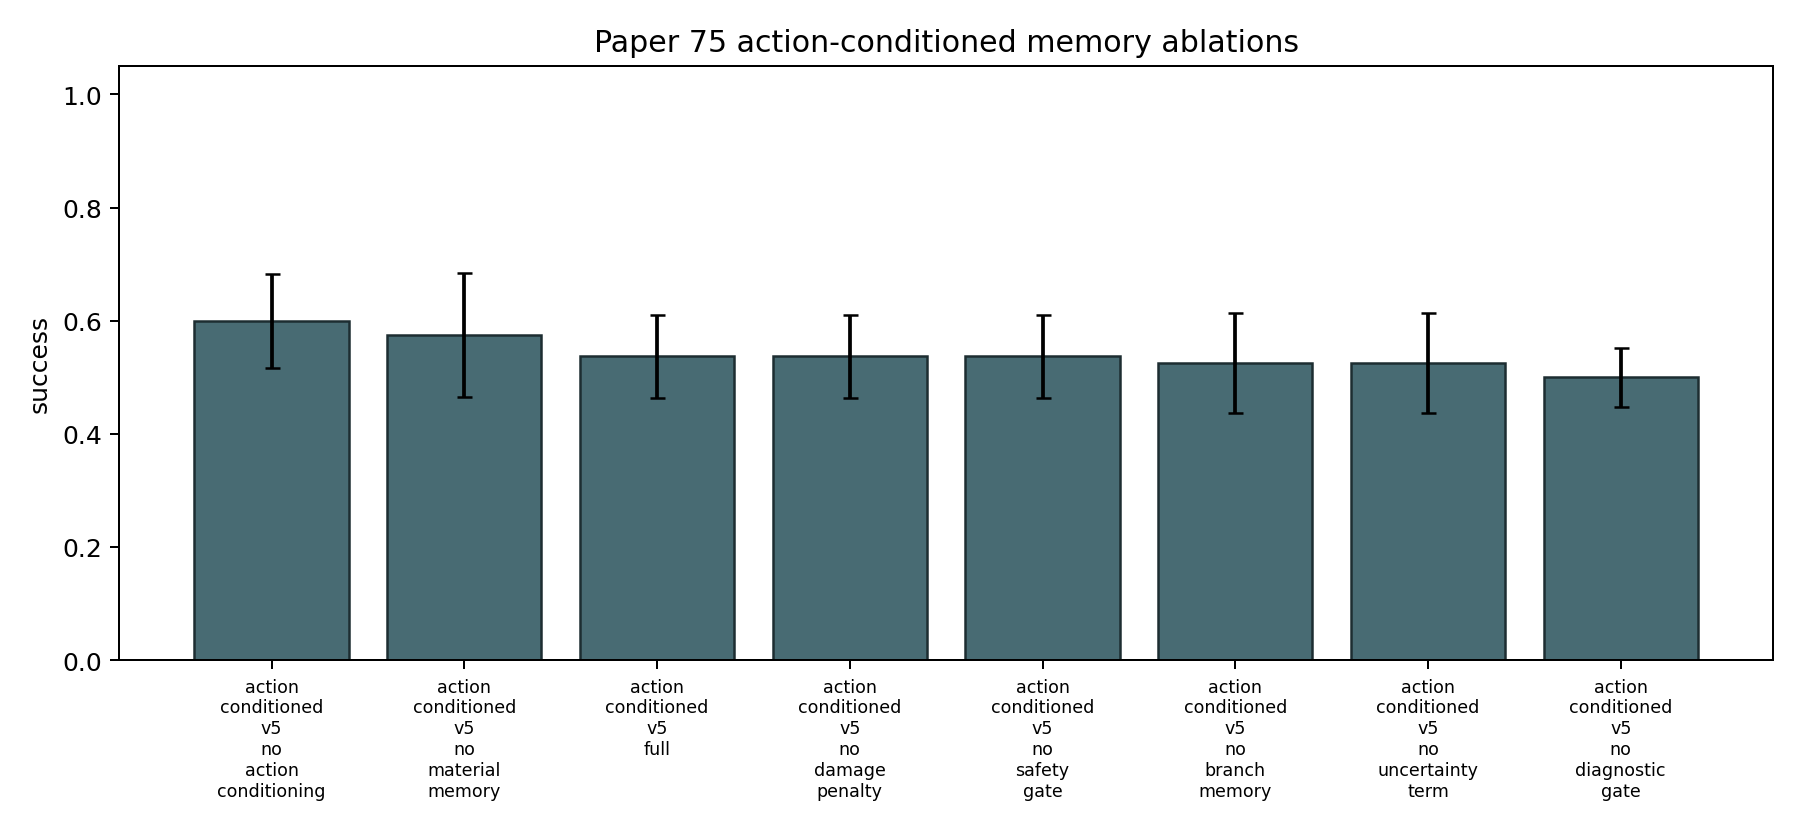
\includegraphics[width=0.92\linewidth]{../figures/deformable_memory_ablation_success.png}
\caption{Ablation success for v5 components on combined memory stress.}
\end{figure}
\scriptsize
\setlength{\tabcolsep}{2pt}
\begin{center}
\refstepcounter{table}\label{tab:ablation}\textbf{Table \thetable: V5 ablations.}\\[0.4ex]
\begin{tabular}{lccccc}
\toprule
ablation & success & damage & mem err & mech F1 & diag \\
\midrule
\texttt{no-action} & $0.600 \pm 0.083$ & $0.212 \pm 0.094$ & $0.523 \pm 0.051$ & $0.438 \pm 0.065$ & $0.000 \pm 0.000$ \\
\texttt{no-material} & $0.575 \pm 0.110$ & $0.263 \pm 0.111$ & $0.237 \pm 0.017$ & $0.469 \pm 0.077$ & $0.000 \pm 0.000$ \\
\texttt{full-v5} & $0.537 \pm 0.073$ & $0.275 \pm 0.103$ & $0.266 \pm 0.028$ & $0.453 \pm 0.064$ & $0.000 \pm 0.000$ \\
\texttt{no-damage} & $0.537 \pm 0.073$ & $0.275 \pm 0.103$ & $0.266 \pm 0.028$ & $0.453 \pm 0.064$ & $0.000 \pm 0.000$ \\
\texttt{no-safety} & $0.537 \pm 0.073$ & $0.275 \pm 0.103$ & $0.266 \pm 0.028$ & $0.453 \pm 0.064$ & $0.000 \pm 0.000$ \\
\texttt{no-branch} & $0.525 \pm 0.089$ & $0.287 \pm 0.078$ & $0.266 \pm 0.028$ & $0.539 \pm 0.069$ & $0.000 \pm 0.000$ \\
\texttt{no-uncertainty} & $0.525 \pm 0.089$ & $0.287 \pm 0.078$ & $0.266 \pm 0.028$ & $0.539 \pm 0.069$ & $0.000 \pm 0.000$ \\
\texttt{no-diag-gate} & $0.500 \pm 0.052$ & $0.287 \pm 0.094$ & $0.266 \pm 0.028$ & $0.453 \pm 0.064$ & $0.138 \pm 0.063$ \\
\bottomrule
\end{tabular}
\end{center}
\normalsize

\section{Stress Sweep}
\begin{figure}[t]
\centering
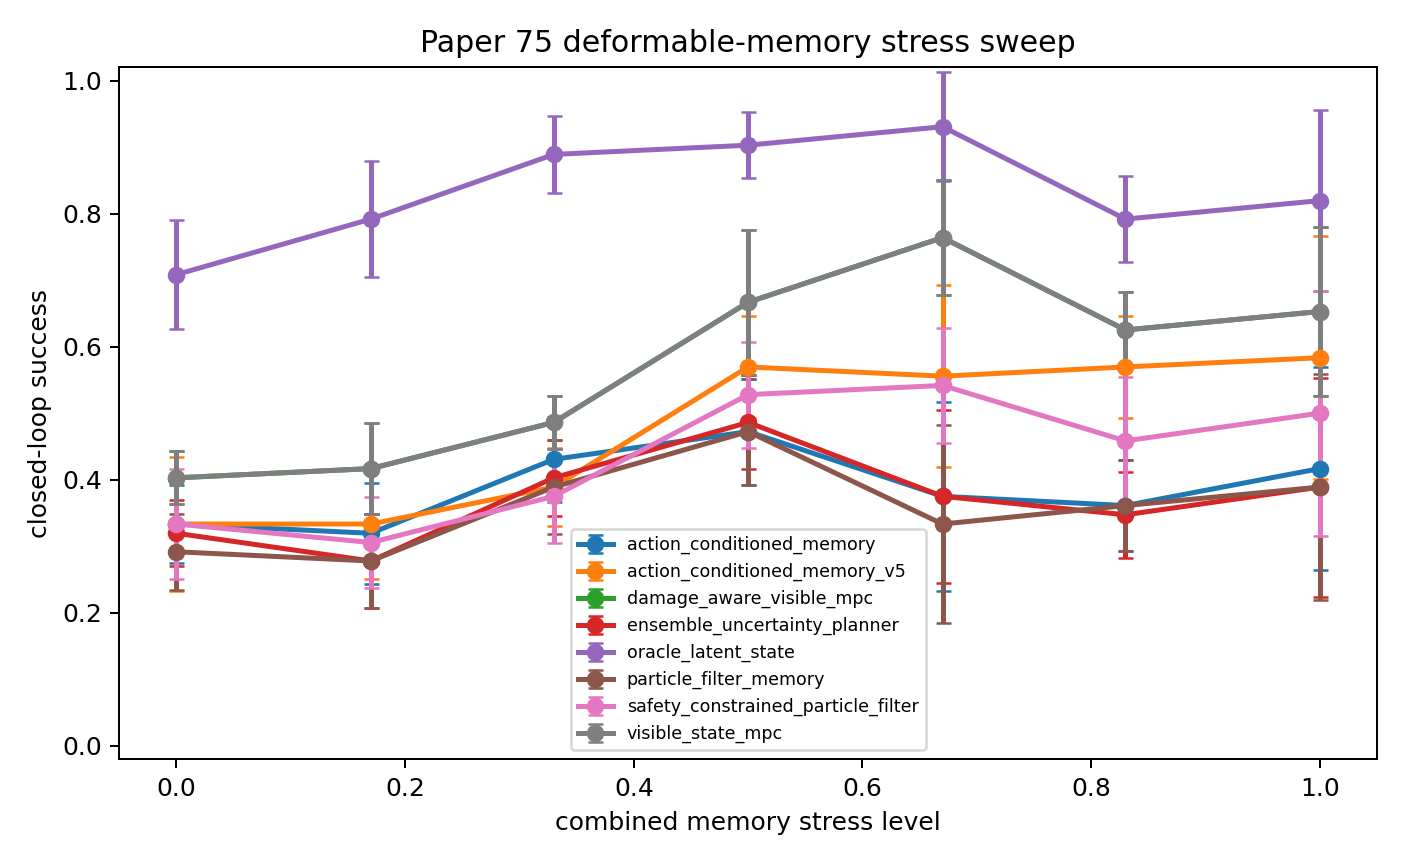
\includegraphics[width=0.92\linewidth]{../figures/deformable_memory_stress_sweep.png}
\caption{Stress sweep over combined hidden strain, occlusion, material shift, fixture strength, force limits, and observation noise.}
\end{figure}

At maximum stress level 1.00, \texttt{ACM-v5} reaches $0.583 \pm 0.183$ success, while the strongest non-oracle stress baseline, \texttt{damage-visible}, reaches $0.653 \pm 0.126$. This gate is reported even if it is unfavorable.

\scriptsize
\setlength{\tabcolsep}{2pt}
\begin{center}
\refstepcounter{table}\label{tab:stress}\textbf{Table \thetable: Stress sweep metrics.}\\[0.4ex]
\begin{tabular}{lccccc}
\toprule
method & level & success & damage & clip & diag \\
\midrule
\texttt{ACM-v4} & 0.00 & $0.333 \pm 0.058$ & $0.347 \pm 0.076$ & $0.001 \pm 0.001$ & $0.792 \pm 0.104$ \\
\texttt{ACM-v5} & 0.00 & $0.333 \pm 0.101$ & $0.264 \pm 0.091$ & $0.007 \pm 0.002$ & $0.000 \pm 0.000$ \\
\texttt{damage-visible} & 0.00 & $0.403 \pm 0.040$ & $0.264 \pm 0.040$ & $0.008 \pm 0.002$ & $0.000 \pm 0.000$ \\
\texttt{ensemble} & 0.00 & $0.319 \pm 0.049$ & $0.347 \pm 0.076$ & $0.002 \pm 0.001$ & $0.750 \pm 0.090$ \\
\texttt{oracle} & 0.00 & $0.708 \pm 0.082$ & $0.000 \pm 0.000$ & $0.001 \pm 0.001$ & $0.000 \pm 0.000$ \\
\texttt{particle} & 0.00 & $0.292 \pm 0.057$ & $0.389 \pm 0.058$ & $0.000 \pm 0.001$ & $0.889 \pm 0.058$ \\
\texttt{safe-particle} & 0.00 & $0.333 \pm 0.082$ & $0.292 \pm 0.040$ & $0.008 \pm 0.002$ & $0.028 \pm 0.036$ \\
\texttt{visible-MPC} & 0.00 & $0.403 \pm 0.040$ & $0.264 \pm 0.040$ & $0.008 \pm 0.002$ & $0.000 \pm 0.000$ \\
\texttt{ACM-v4} & 0.17 & $0.319 \pm 0.076$ & $0.347 \pm 0.087$ & $0.006 \pm 0.001$ & $0.917 \pm 0.054$ \\
\texttt{ACM-v5} & 0.17 & $0.333 \pm 0.082$ & $0.250 \pm 0.068$ & $0.011 \pm 0.001$ & $0.000 \pm 0.000$ \\
\texttt{damage-visible} & 0.17 & $0.417 \pm 0.068$ & $0.250 \pm 0.036$ & $0.011 \pm 0.001$ & $0.000 \pm 0.000$ \\
\texttt{ensemble} & 0.17 & $0.278 \pm 0.071$ & $0.361 \pm 0.080$ & $0.006 \pm 0.001$ & $0.861 \pm 0.099$ \\
\texttt{oracle} & 0.17 & $0.792 \pm 0.087$ & $0.014 \pm 0.027$ & $0.003 \pm 0.001$ & $0.000 \pm 0.000$ \\
\texttt{particle} & 0.17 & $0.278 \pm 0.071$ & $0.389 \pm 0.058$ & $0.005 \pm 0.001$ & $1.000 \pm 0.000$ \\
\texttt{safe-particle} & 0.17 & $0.306 \pm 0.068$ & $0.278 \pm 0.058$ & $0.010 \pm 0.001$ & $0.125 \pm 0.076$ \\
\texttt{visible-MPC} & 0.17 & $0.417 \pm 0.068$ & $0.250 \pm 0.036$ & $0.011 \pm 0.001$ & $0.000 \pm 0.000$ \\
\texttt{ACM-v4} & 0.33 & $0.431 \pm 0.064$ & $0.417 \pm 0.068$ & $0.009 \pm 0.002$ & $0.917 \pm 0.054$ \\
\texttt{ACM-v5} & 0.33 & $0.389 \pm 0.058$ & $0.250 \pm 0.099$ & $0.015 \pm 0.002$ & $0.000 \pm 0.000$ \\
\texttt{damage-visible} & 0.33 & $0.486 \pm 0.040$ & $0.250 \pm 0.036$ & $0.016 \pm 0.001$ & $0.000 \pm 0.000$ \\
\texttt{ensemble} & 0.33 & $0.403 \pm 0.057$ & $0.403 \pm 0.071$ & $0.009 \pm 0.002$ & $0.875 \pm 0.087$ \\
\texttt{oracle} & 0.33 & $0.889 \pm 0.058$ & $0.014 \pm 0.027$ & $0.006 \pm 0.002$ & $0.014 \pm 0.027$ \\
\texttt{particle} & 0.33 & $0.389 \pm 0.071$ & $0.444 \pm 0.058$ & $0.009 \pm 0.002$ & $0.986 \pm 0.027$ \\
\texttt{safe-particle} & 0.33 & $0.375 \pm 0.071$ & $0.292 \pm 0.100$ & $0.013 \pm 0.002$ & $0.250 \pm 0.068$ \\
\texttt{visible-MPC} & 0.33 & $0.486 \pm 0.040$ & $0.250 \pm 0.036$ & $0.016 \pm 0.001$ & $0.000 \pm 0.000$ \\
\texttt{ACM-v4} & 0.50 & $0.472 \pm 0.080$ & $0.431 \pm 0.064$ & $0.019 \pm 0.002$ & $0.972 \pm 0.036$ \\
\texttt{ACM-v5} & 0.50 & $0.569 \pm 0.076$ & $0.250 \pm 0.080$ & $0.022 \pm 0.003$ & $0.000 \pm 0.000$ \\
\texttt{damage-visible} & 0.50 & $0.667 \pm 0.109$ & $0.208 \pm 0.064$ & $0.024 \pm 0.001$ & $0.000 \pm 0.000$ \\
\texttt{ensemble} & 0.50 & $0.486 \pm 0.071$ & $0.417 \pm 0.054$ & $0.020 \pm 0.001$ & $0.944 \pm 0.058$ \\
\bottomrule
\end{tabular}
\end{center}
\begin{center}
\textbf{Table \ref{tab:stress} continued}\\[0.4ex]
\begin{tabular}{lccccc}
\toprule
method & level & success & damage & clip & diag \\
\midrule
\texttt{oracle} & 0.50 & $0.903 \pm 0.049$ & $0.028 \pm 0.036$ & $0.011 \pm 0.002$ & $0.000 \pm 0.000$ \\
\texttt{particle} & 0.50 & $0.472 \pm 0.080$ & $0.431 \pm 0.064$ & $0.020 \pm 0.001$ & $1.000 \pm 0.000$ \\
\texttt{safe-particle} & 0.50 & $0.528 \pm 0.080$ & $0.278 \pm 0.071$ & $0.021 \pm 0.003$ & $0.347 \pm 0.096$ \\
\texttt{visible-MPC} & 0.50 & $0.667 \pm 0.109$ & $0.208 \pm 0.064$ & $0.024 \pm 0.001$ & $0.000 \pm 0.000$ \\
\texttt{ACM-v4} & 0.67 & $0.375 \pm 0.142$ & $0.556 \pm 0.165$ & $0.025 \pm 0.002$ & $0.917 \pm 0.068$ \\
\texttt{ACM-v5} & 0.67 & $0.556 \pm 0.137$ & $0.264 \pm 0.082$ & $0.024 \pm 0.003$ & $0.000 \pm 0.000$ \\
\texttt{damage-visible} & 0.67 & $0.764 \pm 0.087$ & $0.139 \pm 0.068$ & $0.030 \pm 0.002$ & $0.000 \pm 0.000$ \\
\texttt{ensemble} & 0.67 & $0.375 \pm 0.130$ & $0.556 \pm 0.148$ & $0.025 \pm 0.002$ & $0.917 \pm 0.054$ \\
\texttt{oracle} & 0.67 & $0.931 \pm 0.082$ & $0.014 \pm 0.027$ & $0.016 \pm 0.004$ & $0.000 \pm 0.000$ \\
\texttt{particle} & 0.67 & $0.333 \pm 0.148$ & $0.625 \pm 0.164$ & $0.024 \pm 0.002$ & $0.986 \pm 0.027$ \\
\texttt{safe-particle} & 0.67 & $0.542 \pm 0.087$ & $0.278 \pm 0.082$ & $0.026 \pm 0.003$ & $0.389 \pm 0.130$ \\
\texttt{visible-MPC} & 0.67 & $0.764 \pm 0.087$ & $0.139 \pm 0.068$ & $0.030 \pm 0.002$ & $0.000 \pm 0.000$ \\
\texttt{ACM-v4} & 0.83 & $0.361 \pm 0.068$ & $0.597 \pm 0.071$ & $0.037 \pm 0.002$ & $0.958 \pm 0.057$ \\
\texttt{ACM-v5} & 0.83 & $0.569 \pm 0.076$ & $0.292 \pm 0.071$ & $0.027 \pm 0.004$ & $0.000 \pm 0.000$ \\
\texttt{damage-visible} & 0.83 & $0.625 \pm 0.057$ & $0.264 \pm 0.057$ & $0.036 \pm 0.002$ & $0.000 \pm 0.000$ \\
\texttt{ensemble} & 0.83 & $0.347 \pm 0.064$ & $0.611 \pm 0.071$ & $0.036 \pm 0.003$ & $0.986 \pm 0.027$ \\
\texttt{oracle} & 0.83 & $0.792 \pm 0.064$ & $0.083 \pm 0.068$ & $0.024 \pm 0.003$ & $0.028 \pm 0.036$ \\
\texttt{particle} & 0.83 & $0.361 \pm 0.068$ & $0.597 \pm 0.082$ & $0.037 \pm 0.002$ & $0.972 \pm 0.036$ \\
\texttt{safe-particle} & 0.83 & $0.458 \pm 0.096$ & $0.417 \pm 0.122$ & $0.033 \pm 0.003$ & $0.500 \pm 0.123$ \\
\texttt{visible-MPC} & 0.83 & $0.625 \pm 0.057$ & $0.264 \pm 0.057$ & $0.036 \pm 0.002$ & $0.000 \pm 0.000$ \\
\texttt{ACM-v4} & 1.00 & $0.417 \pm 0.153$ & $0.542 \pm 0.172$ & $0.050 \pm 0.003$ & $0.972 \pm 0.036$ \\
\texttt{ACM-v5} & 1.00 & $0.583 \pm 0.183$ & $0.333 \pm 0.179$ & $0.037 \pm 0.005$ & $0.000 \pm 0.000$ \\
\texttt{damage-visible} & 1.00 & $0.653 \pm 0.126$ & $0.236 \pm 0.139$ & $0.046 \pm 0.002$ & $0.000 \pm 0.000$ \\
\texttt{ensemble} & 1.00 & $0.389 \pm 0.165$ & $0.569 \pm 0.186$ & $0.049 \pm 0.003$ & $0.958 \pm 0.040$ \\
\texttt{oracle} & 1.00 & $0.819 \pm 0.136$ & $0.083 \pm 0.080$ & $0.033 \pm 0.005$ & $0.028 \pm 0.036$ \\
\texttt{particle} & 1.00 & $0.389 \pm 0.170$ & $0.569 \pm 0.186$ & $0.049 \pm 0.003$ & $0.958 \pm 0.040$ \\
\texttt{safe-particle} & 1.00 & $0.500 \pm 0.184$ & $0.389 \pm 0.210$ & $0.045 \pm 0.002$ & $0.444 \pm 0.082$ \\
\texttt{visible-MPC} & 1.00 & $0.653 \pm 0.126$ & $0.236 \pm 0.139$ & $0.046 \pm 0.002$ & $0.000 \pm 0.000$ \\
\bottomrule
\end{tabular}
\end{center}
\normalsize

\section{Negative Cases}
Negative cases are not anecdotes used to excuse the result; they are scenario-level checks that the average tables do not hide systematic failure modes. When a successful non-oracle baseline exists on the same scenario, the table lists it.

\tiny
\setlength{\tabcolsep}{2pt}
\begin{center}
\refstepcounter{table}\label{tab:negative}\textbf{Table \thetable: Scenario-level negative cases for v5.}\\[0.4ex]
\begin{tabular}{lllllp{0.24\linewidth}c}
\toprule
seed & object & v5 action & successful baseline & baseline action & failures & shape \\
\midrule
0 & rope & fixture\_avoid\_pull &  &  & branch,shape & 0.187 \\
0 & cloth\_strip & gentle\_relax\_pull &  &  & snag & 0.147 \\
0 & deformable\_sheet & fixture\_avoid\_pull &  &  & snag & 0.147 \\
0 & rope & fixture\_avoid\_pull &  &  & stretch,occ & 0.171 \\
0 & rope & fixture\_avoid\_pull &  &  & branch,occ,shape & 0.191 \\
0 & cloth\_strip & fixture\_avoid\_pull &  &  & occ,shape & 0.161 \\
1 & rope & fixture\_avoid\_pull &  &  & stretch & 0.173 \\
1 & cloth\_strip & fixture\_avoid\_pull & \texttt{graph} & gentle\_relax\_pull & shape & 0.165 \\
1 & rope & fixture\_avoid\_pull &  &  & stretch,occ & 0.171 \\
1 & elastic\_band & gentle\_relax\_pull & \texttt{visible-MPC} & fixture\_avoid\_pull & snag & 0.093 \\
1 & rope & fixture\_avoid\_pull &  &  & stretch,branch,shape & 0.196 \\
1 & cloth\_strip & fixture\_avoid\_pull & \texttt{history} & diagnostic\_branch\_pull & occ,shape & 0.162 \\
\bottomrule
\end{tabular}
\end{center}
\normalsize

\section{Limitations}
This artifact is not a real-robot paper. It has no hardware videos, no public deformable benchmark, no tactile sensing, no RGBD perception stack, and no large neural dynamics model. It uses Ridge regressors from scikit-learn \citep{pedregosa2011scikit} and a local simulator so that the evidence is cheap, reproducible, and easy to audit. Those constraints are deliberate, but they limit external validity. The right conclusion is not that deformable memory is useless; it is that this specific action-conditioned memory planner is not yet a submission-worthy control result.

\section{Conclusion}
The v5 rebuild improves the scientific artifact and sharpens the negative result. It adds the theory that v4 was missing, tries the obvious safety-gated rescue, evaluates stronger baselines, reports fixed-risk and stress behavior, and preserves failures. The frozen decision remains \textbf{KILL\_ARCHIVE}. A future revival would need either safer diagnostic actions, a richer low-risk action library, hardware validation, or a learned dynamics model that turns hidden memory into a consistent closed-loop advantage.

\clearpage
\appendix
\section{Full Main Metrics}
\scriptsize
\setlength{\tabcolsep}{2pt}
\begin{center}
\refstepcounter{table}\label{tab:main-all}\textbf{Table \thetable: All method/split main metrics.}\\[0.4ex]
\begin{tabular}{llccccc}
\toprule
method & split & success & damage & mem err & mech F1 & diag \\
\midrule
\texttt{oracle} & \texttt{combined} & $0.821 \pm 0.084$ & $0.062 \pm 0.041$ & $0.000 \pm 0.000$ & $1.000 \pm 0.000$ & $0.018 \pm 0.023$ \\
\texttt{damage-visible} & \texttt{combined} & $0.589 \pm 0.058$ & $0.205 \pm 0.041$ & $0.578 \pm 0.018$ & $0.406 \pm 0.040$ & $0.000 \pm 0.000$ \\
\texttt{visible-MPC} & \texttt{combined} & $0.589 \pm 0.058$ & $0.205 \pm 0.041$ & $0.578 \pm 0.018$ & $0.406 \pm 0.040$ & $0.000 \pm 0.000$ \\
\texttt{ACM-v5} & \texttt{combined} & $0.562 \pm 0.062$ & $0.250 \pm 0.075$ & $0.229 \pm 0.031$ & $0.438 \pm 0.065$ & $0.000 \pm 0.000$ \\
\texttt{graph} & \texttt{combined} & $0.536 \pm 0.092$ & $0.259 \pm 0.064$ & $0.525 \pm 0.032$ & $0.427 \pm 0.043$ & $0.000 \pm 0.000$ \\
\texttt{safe-particle} & \texttt{combined} & $0.518 \pm 0.063$ & $0.330 \pm 0.064$ & $0.256 \pm 0.031$ & $0.391 \pm 0.031$ & $0.446 \pm 0.069$ \\
\texttt{robust-CEM} & \texttt{combined} & $0.482 \pm 0.058$ & $0.420 \pm 0.041$ & $0.255 \pm 0.031$ & $0.406 \pm 0.040$ & $0.786 \pm 0.070$ \\
\texttt{ACM-v4} & \texttt{combined} & $0.446 \pm 0.063$ & $0.482 \pm 0.051$ & $0.206 \pm 0.032$ & $0.453 \pm 0.045$ & $0.955 \pm 0.026$ \\
\texttt{history} & \texttt{combined} & $0.438 \pm 0.062$ & $0.482 \pm 0.035$ & $0.187 \pm 0.029$ & $0.438 \pm 0.046$ & $0.929 \pm 0.037$ \\
\texttt{particle} & \texttt{combined} & $0.438 \pm 0.056$ & $0.500 \pm 0.046$ & $0.187 \pm 0.029$ & $0.500 \pm 0.000$ & $0.964 \pm 0.026$ \\
\texttt{ensemble} & \texttt{combined} & $0.429 \pm 0.059$ & $0.500 \pm 0.037$ & $0.187 \pm 0.030$ & $0.469 \pm 0.040$ & $0.973 \pm 0.026$ \\
\texttt{oracle} & \texttt{hidden-strain} & $0.893 \pm 0.046$ & $0.027 \pm 0.026$ & $0.000 \pm 0.000$ & $1.000 \pm 0.000$ & $0.000 \pm 0.000$ \\
\texttt{damage-visible} & \texttt{hidden-strain} & $0.536 \pm 0.059$ & $0.241 \pm 0.037$ & $0.480 \pm 0.009$ & $0.578 \pm 0.045$ & $0.000 \pm 0.000$ \\
\texttt{visible-MPC} & \texttt{hidden-strain} & $0.536 \pm 0.059$ & $0.241 \pm 0.037$ & $0.480 \pm 0.009$ & $0.578 \pm 0.045$ & $0.000 \pm 0.000$ \\
\texttt{graph} & \texttt{hidden-strain} & $0.473 \pm 0.037$ & $0.205 \pm 0.062$ & $0.382 \pm 0.029$ & $0.578 \pm 0.045$ & $0.000 \pm 0.000$ \\
\texttt{history} & \texttt{hidden-strain} & $0.446 \pm 0.063$ & $0.420 \pm 0.049$ & $0.180 \pm 0.024$ & $0.594 \pm 0.061$ & $0.884 \pm 0.059$ \\
\texttt{ACM-v4} & \texttt{hidden-strain} & $0.429 \pm 0.065$ & $0.438 \pm 0.049$ & $0.189 \pm 0.028$ & $0.609 \pm 0.056$ & $0.893 \pm 0.046$ \\
\texttt{ensemble} & \texttt{hidden-strain} & $0.429 \pm 0.065$ & $0.438 \pm 0.041$ & $0.183 \pm 0.024$ & $0.578 \pm 0.045$ & $0.911 \pm 0.058$ \\
\texttt{safe-particle} & \texttt{hidden-strain} & $0.420 \pm 0.049$ & $0.232 \pm 0.044$ & $0.209 \pm 0.027$ & $0.568 \pm 0.051$ & $0.009 \pm 0.018$ \\
\texttt{robust-CEM} & \texttt{hidden-strain} & $0.411 \pm 0.074$ & $0.330 \pm 0.052$ & $0.210 \pm 0.027$ & $0.594 \pm 0.040$ & $0.464 \pm 0.106$ \\
\texttt{particle} & \texttt{hidden-strain} & $0.402 \pm 0.064$ & $0.464 \pm 0.046$ & $0.180 \pm 0.024$ & $0.609 \pm 0.031$ & $0.902 \pm 0.052$ \\
\texttt{ACM-v5} & \texttt{hidden-strain} & $0.393 \pm 0.053$ & $0.241 \pm 0.052$ & $0.198 \pm 0.028$ & $0.552 \pm 0.051$ & $0.000 \pm 0.000$ \\
\texttt{oracle} & \texttt{material-shift} & $0.920 \pm 0.041$ & $0.000 \pm 0.000$ & $0.000 \pm 0.000$ & $1.000 \pm 0.000$ & $0.018 \pm 0.023$ \\
\texttt{damage-visible} & \texttt{material-shift} & $0.491 \pm 0.049$ & $0.214 \pm 0.037$ & $0.295 \pm 0.004$ & $0.625 \pm 0.000$ & $0.000 \pm 0.000$ \\
\bottomrule
\end{tabular}
\end{center}
\begin{center}
\textbf{Table \ref{tab:main-all} continued}\\[0.4ex]
\begin{tabular}{llccccc}
\toprule
method & split & success & damage & mem err & mech F1 & diag \\
\midrule
\texttt{visible-MPC} & \texttt{material-shift} & $0.491 \pm 0.049$ & $0.214 \pm 0.037$ & $0.295 \pm 0.004$ & $0.625 \pm 0.000$ & $0.000 \pm 0.000$ \\
\texttt{graph} & \texttt{material-shift} & $0.420 \pm 0.077$ & $0.205 \pm 0.062$ & $0.271 \pm 0.030$ & $0.594 \pm 0.040$ & $0.000 \pm 0.000$ \\
\texttt{history} & \texttt{material-shift} & $0.384 \pm 0.079$ & $0.438 \pm 0.081$ & $0.150 \pm 0.016$ & $0.516 \pm 0.031$ & $0.777 \pm 0.081$ \\
\texttt{safe-particle} & \texttt{material-shift} & $0.375 \pm 0.069$ & $0.241 \pm 0.059$ & $0.165 \pm 0.016$ & $0.562 \pm 0.046$ & $0.054 \pm 0.044$ \\
\texttt{ACM-v4} & \texttt{material-shift} & $0.366 \pm 0.072$ & $0.473 \pm 0.083$ & $0.153 \pm 0.015$ & $0.516 \pm 0.031$ & $0.812 \pm 0.052$ \\
\texttt{ACM-v5} & \texttt{material-shift} & $0.366 \pm 0.072$ & $0.214 \pm 0.070$ & $0.157 \pm 0.016$ & $0.578 \pm 0.045$ & $0.000 \pm 0.000$ \\
\texttt{ensemble} & \texttt{material-shift} & $0.366 \pm 0.072$ & $0.464 \pm 0.088$ & $0.152 \pm 0.016$ & $0.516 \pm 0.031$ & $0.777 \pm 0.041$ \\
\texttt{robust-CEM} & \texttt{material-shift} & $0.366 \pm 0.072$ & $0.304 \pm 0.058$ & $0.165 \pm 0.016$ & $0.516 \pm 0.031$ & $0.348 \pm 0.072$ \\
\texttt{particle} & \texttt{material-shift} & $0.348 \pm 0.085$ & $0.509 \pm 0.097$ & $0.150 \pm 0.016$ & $0.578 \pm 0.045$ & $0.955 \pm 0.045$ \\
\texttt{oracle} & \texttt{nominal} & $0.705 \pm 0.062$ & $0.000 \pm 0.000$ & $0.000 \pm 0.000$ & $1.000 \pm 0.000$ & $0.000 \pm 0.000$ \\
\texttt{damage-visible} & \texttt{nominal} & $0.393 \pm 0.070$ & $0.250 \pm 0.026$ & $0.124 \pm 0.003$ & $0.625 \pm 0.000$ & $0.000 \pm 0.000$ \\
\texttt{visible-MPC} & \texttt{nominal} & $0.393 \pm 0.070$ & $0.250 \pm 0.026$ & $0.124 \pm 0.003$ & $0.625 \pm 0.000$ & $0.000 \pm 0.000$ \\
\texttt{graph} & \texttt{nominal} & $0.384 \pm 0.070$ & $0.214 \pm 0.046$ & $0.109 \pm 0.013$ & $0.625 \pm 0.000$ & $0.000 \pm 0.000$ \\
\texttt{ACM-v4} & \texttt{nominal} & $0.366 \pm 0.077$ & $0.259 \pm 0.026$ & $0.111 \pm 0.022$ & $0.609 \pm 0.031$ & $0.214 \pm 0.065$ \\
\texttt{ACM-v5} & \texttt{nominal} & $0.366 \pm 0.067$ & $0.232 \pm 0.035$ & $0.104 \pm 0.021$ & $0.625 \pm 0.000$ & $0.000 \pm 0.000$ \\
\texttt{safe-particle} & \texttt{nominal} & $0.366 \pm 0.067$ & $0.250 \pm 0.026$ & $0.099 \pm 0.018$ & $0.625 \pm 0.000$ & $0.000 \pm 0.000$ \\
\texttt{robust-CEM} & \texttt{nominal} & $0.357 \pm 0.075$ & $0.250 \pm 0.026$ & $0.099 \pm 0.019$ & $0.625 \pm 0.000$ & $0.045 \pm 0.026$ \\
\texttt{ensemble} & \texttt{nominal} & $0.348 \pm 0.056$ & $0.268 \pm 0.023$ & $0.128 \pm 0.024$ & $0.594 \pm 0.040$ & $0.339 \pm 0.063$ \\
\texttt{history} & \texttt{nominal} & $0.348 \pm 0.056$ & $0.259 \pm 0.026$ & $0.126 \pm 0.021$ & $0.609 \pm 0.031$ & $0.250 \pm 0.059$ \\
\texttt{particle} & \texttt{nominal} & $0.348 \pm 0.049$ & $0.295 \pm 0.032$ & $0.126 \pm 0.021$ & $0.547 \pm 0.045$ & $0.545 \pm 0.091$ \\
\texttt{oracle} & \texttt{occluded-contact} & $0.830 \pm 0.070$ & $0.018 \pm 0.023$ & $0.000 \pm 0.000$ & $1.000 \pm 0.000$ & $0.000 \pm 0.000$ \\
\texttt{damage-visible} & \texttt{occluded-contact} & $0.536 \pm 0.046$ & $0.250 \pm 0.026$ & $0.393 \pm 0.009$ & $0.453 \pm 0.045$ & $0.000 \pm 0.000$ \\
\texttt{visible-MPC} & \texttt{occluded-contact} & $0.536 \pm 0.046$ & $0.250 \pm 0.026$ & $0.393 \pm 0.009$ & $0.453 \pm 0.045$ & $0.000 \pm 0.000$ \\
\texttt{safe-particle} & \texttt{occluded-contact} & $0.446 \pm 0.035$ & $0.295 \pm 0.032$ & $0.211 \pm 0.026$ & $0.406 \pm 0.040$ & $0.071 \pm 0.053$ \\
\bottomrule
\end{tabular}
\end{center}
\begin{center}
\textbf{Table \ref{tab:main-all} continued}\\[0.4ex]
\begin{tabular}{llccccc}
\toprule
method & split & success & damage & mem err & mech F1 & diag \\
\midrule
\texttt{ACM-v5} & \texttt{occluded-contact} & $0.420 \pm 0.062$ & $0.295 \pm 0.041$ & $0.203 \pm 0.023$ & $0.438 \pm 0.046$ & $0.000 \pm 0.000$ \\
\texttt{graph} & \texttt{occluded-contact} & $0.420 \pm 0.041$ & $0.304 \pm 0.035$ & $0.357 \pm 0.038$ & $0.391 \pm 0.031$ & $0.000 \pm 0.000$ \\
\texttt{robust-CEM} & \texttt{occluded-contact} & $0.420 \pm 0.049$ & $0.339 \pm 0.051$ & $0.211 \pm 0.026$ & $0.406 \pm 0.040$ & $0.384 \pm 0.083$ \\
\texttt{history} & \texttt{occluded-contact} & $0.393 \pm 0.046$ & $0.500 \pm 0.059$ & $0.197 \pm 0.024$ & $0.453 \pm 0.045$ & $0.839 \pm 0.063$ \\
\texttt{ACM-v4} & \texttt{occluded-contact} & $0.384 \pm 0.064$ & $0.482 \pm 0.044$ & $0.199 \pm 0.022$ & $0.422 \pm 0.045$ & $0.795 \pm 0.056$ \\
\texttt{ensemble} & \texttt{occluded-contact} & $0.384 \pm 0.064$ & $0.491 \pm 0.041$ & $0.200 \pm 0.025$ & $0.438 \pm 0.046$ & $0.812 \pm 0.059$ \\
\texttt{particle} & \texttt{occluded-contact} & $0.357 \pm 0.075$ & $0.545 \pm 0.064$ & $0.197 \pm 0.024$ & $0.469 \pm 0.040$ & $0.929 \pm 0.026$ \\
\bottomrule
\end{tabular}
\end{center}
\normalsize

\section{Full Pairwise Comparisons}
\scriptsize
\setlength{\tabcolsep}{2pt}
\begin{center}
\refstepcounter{table}\label{tab:pairwise}\textbf{Table \thetable: Pairwise v5-minus-comparison statistics by split.}\\[0.4ex]
\begin{tabular}{llcccccc}
\toprule
split & comparison & d success & CI & mem red & F1 diff & dmg red & better \\
\midrule
\texttt{combined} & \texttt{ACM-v4} & 0.116 & 0.045 & -0.023 & -0.016 & 0.232 & 7/8 \\
\texttt{combined} & \texttt{damage-visible} & -0.027 & 0.052 & 0.349 & 0.031 & -0.045 & 2/8 \\
\texttt{combined} & \texttt{ensemble} & 0.134 & 0.056 & -0.042 & -0.031 & 0.250 & 7/8 \\
\texttt{combined} & \texttt{graph} & 0.027 & 0.087 & 0.296 & 0.010 & 0.009 & 4/8 \\
\texttt{combined} & \texttt{history} & 0.125 & 0.051 & -0.042 & 0.000 & 0.232 & 7/8 \\
\texttt{combined} & \texttt{oracle} & -0.259 & 0.083 & -0.229 & -0.562 & -0.188 & 0/8 \\
\texttt{combined} & \texttt{particle} & 0.125 & 0.063 & -0.042 & -0.062 & 0.250 & 6/8 \\
\texttt{combined} & \texttt{robust-CEM} & 0.080 & 0.049 & 0.026 & 0.031 & 0.170 & 6/8 \\
\texttt{combined} & \texttt{safe-particle} & 0.045 & 0.037 & 0.027 & 0.047 & 0.080 & 4/8 \\
\texttt{combined} & \texttt{visible-MPC} & -0.027 & 0.052 & 0.349 & 0.031 & -0.045 & 2/8 \\
\texttt{hidden-strain} & \texttt{ACM-v4} & -0.036 & 0.079 & -0.009 & -0.057 & 0.196 & 3/8 \\
\texttt{hidden-strain} & \texttt{damage-visible} & -0.143 & 0.070 & 0.282 & -0.026 & 0.000 & 0/8 \\
\texttt{hidden-strain} & \texttt{ensemble} & -0.036 & 0.079 & -0.015 & -0.026 & 0.196 & 2/8 \\
\texttt{hidden-strain} & \texttt{graph} & -0.080 & 0.041 & 0.184 & -0.026 & -0.036 & 0/8 \\
\texttt{hidden-strain} & \texttt{history} & -0.054 & 0.074 & -0.018 & -0.042 & 0.179 & 2/8 \\
\texttt{hidden-strain} & \texttt{oracle} & -0.500 & 0.059 & -0.198 & -0.448 & -0.214 & 0/8 \\
\texttt{hidden-strain} & \texttt{particle} & -0.009 & 0.089 & -0.018 & -0.057 & 0.223 & 3/8 \\
\texttt{hidden-strain} & \texttt{robust-CEM} & -0.018 & 0.069 & 0.012 & -0.042 & 0.089 & 2/8 \\
\texttt{hidden-strain} & \texttt{safe-particle} & -0.027 & 0.026 & 0.011 & -0.016 & -0.009 & 0/8 \\
\texttt{hidden-strain} & \texttt{visible-MPC} & -0.143 & 0.070 & 0.282 & -0.026 & 0.000 & 0/8 \\
\texttt{material-shift} & \texttt{ACM-v4} & 0.000 & 0.092 & -0.004 & 0.062 & 0.259 & 3/8 \\
\texttt{material-shift} & \texttt{damage-visible} & -0.125 & 0.051 & 0.138 & -0.047 & 0.000 & 0/8 \\
\texttt{material-shift} & \texttt{ensemble} & 0.000 & 0.095 & -0.005 & 0.062 & 0.250 & 3/8 \\
\texttt{material-shift} & \texttt{graph} & -0.054 & 0.087 & 0.114 & -0.016 & -0.009 & 2/8 \\
\bottomrule
\end{tabular}
\end{center}
\begin{center}
\textbf{Table \ref{tab:pairwise} continued}\\[0.4ex]
\begin{tabular}{llcccccc}
\toprule
split & comparison & d success & CI & mem red & F1 diff & dmg red & better \\
\midrule
\texttt{material-shift} & \texttt{history} & -0.018 & 0.098 & -0.007 & 0.062 & 0.223 & 2/8 \\
\texttt{material-shift} & \texttt{oracle} & -0.554 & 0.051 & -0.157 & -0.422 & -0.214 & 0/8 \\
\texttt{material-shift} & \texttt{particle} & 0.018 & 0.094 & -0.007 & 0.000 & 0.295 & 3/8 \\
\texttt{material-shift} & \texttt{robust-CEM} & 0.000 & 0.079 & 0.008 & 0.062 & 0.089 & 3/8 \\
\texttt{material-shift} & \texttt{safe-particle} & -0.009 & 0.049 & 0.008 & 0.016 & 0.027 & 3/8 \\
\texttt{material-shift} & \texttt{visible-MPC} & -0.125 & 0.051 & 0.138 & -0.047 & 0.000 & 0/8 \\
\texttt{nominal} & \texttt{ACM-v4} & -0.000 & 0.037 & 0.007 & 0.016 & 0.027 & 2/8 \\
\texttt{nominal} & \texttt{damage-visible} & -0.027 & 0.026 & 0.020 & 0.000 & 0.018 & 0/8 \\
\texttt{nominal} & \texttt{ensemble} & 0.018 & 0.044 & 0.024 & 0.031 & 0.036 & 4/8 \\
\texttt{nominal} & \texttt{graph} & -0.018 & 0.023 & 0.005 & 0.000 & -0.018 & 0/8 \\
\texttt{nominal} & \texttt{history} & 0.018 & 0.035 & 0.022 & 0.016 & 0.027 & 3/8 \\
\texttt{nominal} & \texttt{oracle} & -0.339 & 0.035 & -0.104 & -0.375 & -0.232 & 0/8 \\
\texttt{nominal} & \texttt{particle} & 0.018 & 0.035 & 0.022 & 0.078 & 0.062 & 3/8 \\
\texttt{nominal} & \texttt{robust-CEM} & 0.009 & 0.018 & -0.005 & 0.000 & 0.018 & 1/8 \\
\texttt{nominal} & \texttt{safe-particle} & 0.000 & 0.000 & -0.005 & 0.000 & 0.018 & 0/8 \\
\texttt{nominal} & \texttt{visible-MPC} & -0.027 & 0.026 & 0.020 & 0.000 & 0.018 & 0/8 \\
\texttt{occluded-contact} & \texttt{ACM-v4} & 0.036 & 0.088 & -0.004 & 0.016 & 0.188 & 5/8 \\
\texttt{occluded-contact} & \texttt{damage-visible} & -0.116 & 0.045 & 0.190 & -0.016 & -0.045 & 0/8 \\
\texttt{occluded-contact} & \texttt{ensemble} & 0.036 & 0.088 & -0.003 & 0.000 & 0.196 & 5/8 \\
\texttt{occluded-contact} & \texttt{graph} & 0.000 & 0.065 & 0.154 & 0.047 & 0.009 & 2/8 \\
\texttt{occluded-contact} & \texttt{history} & 0.027 & 0.070 & -0.006 & -0.016 & 0.205 & 4/8 \\
\texttt{occluded-contact} & \texttt{oracle} & -0.411 & 0.098 & -0.203 & -0.562 & -0.277 & 0/8 \\
\texttt{occluded-contact} & \texttt{particle} & 0.062 & 0.077 & -0.006 & -0.031 & 0.250 & 5/8 \\
\texttt{occluded-contact} & \texttt{robust-CEM} & 0.000 & 0.053 & 0.009 & 0.031 & 0.045 & 3/8 \\
\bottomrule
\end{tabular}
\end{center}
\begin{center}
\textbf{Table \ref{tab:pairwise} continued}\\[0.4ex]
\begin{tabular}{llcccccc}
\toprule
split & comparison & d success & CI & mem red & F1 diff & dmg red & better \\
\midrule
\texttt{occluded-contact} & \texttt{safe-particle} & -0.027 & 0.045 & 0.008 & 0.031 & -0.000 & 1/8 \\
\texttt{occluded-contact} & \texttt{visible-MPC} & -0.116 & 0.045 & 0.190 & -0.016 & -0.045 & 0/8 \\
\bottomrule
\end{tabular}
\end{center}
\normalsize

\section{Fixed-Risk Pairwise Comparisons}
\scriptsize
\setlength{\tabcolsep}{2pt}
\begin{center}
\refstepcounter{table}\label{tab:fixed-pair}\textbf{Table \thetable: Fixed-risk pairwise comparisons.}\\[0.4ex]
\begin{tabular}{llccccc}
\toprule
split & budget & comparison & d success & CI & dmg red & better \\
\midrule
\texttt{combined} & 0.10 & \texttt{ACM-v4} & 0.078 & 0.092 & 0.078 & 3/8 \\
\texttt{combined} & 0.10 & \texttt{damage-visible} & 0.000 & 0.046 & 0.016 & 1/8 \\
\texttt{combined} & 0.10 & \texttt{ensemble} & 0.094 & 0.101 & 0.078 & 5/8 \\
\texttt{combined} & 0.10 & \texttt{oracle} & -0.203 & 0.079 & -0.109 & 0/8 \\
\texttt{combined} & 0.10 & \texttt{particle} & 0.188 & 0.080 & 0.203 & 7/8 \\
\texttt{combined} & 0.10 & \texttt{robust-CEM} & 0.031 & 0.061 & 0.047 & 1/8 \\
\texttt{combined} & 0.10 & \texttt{safe-particle} & 0.078 & 0.092 & 0.078 & 3/8 \\
\texttt{combined} & 0.10 & \texttt{visible-MPC} & 0.000 & 0.046 & 0.016 & 1/8 \\
\texttt{combined} & 0.20 & \texttt{ACM-v4} & 0.312 & 0.179 & 0.469 & 7/8 \\
\texttt{combined} & 0.20 & \texttt{damage-visible} & 0.000 & 0.046 & 0.016 & 1/8 \\
\texttt{combined} & 0.20 & \texttt{ensemble} & 0.297 & 0.173 & 0.453 & 7/8 \\
\texttt{combined} & 0.20 & \texttt{oracle} & -0.203 & 0.079 & -0.109 & 0/8 \\
\texttt{combined} & 0.20 & \texttt{particle} & 0.312 & 0.179 & 0.469 & 7/8 \\
\texttt{combined} & 0.20 & \texttt{robust-CEM} & 0.188 & 0.131 & 0.297 & 6/8 \\
\texttt{combined} & 0.20 & \texttt{safe-particle} & 0.094 & 0.111 & 0.141 & 4/8 \\
\texttt{combined} & 0.20 & \texttt{visible-MPC} & 0.000 & 0.046 & 0.016 & 1/8 \\
\texttt{combined} & 0.30 & \texttt{ACM-v4} & 0.312 & 0.179 & 0.469 & 7/8 \\
\texttt{combined} & 0.30 & \texttt{damage-visible} & 0.000 & 0.046 & 0.016 & 1/8 \\
\texttt{combined} & 0.30 & \texttt{ensemble} & 0.297 & 0.173 & 0.453 & 7/8 \\
\texttt{combined} & 0.30 & \texttt{oracle} & -0.203 & 0.079 & -0.109 & 0/8 \\
\texttt{combined} & 0.30 & \texttt{particle} & 0.312 & 0.179 & 0.469 & 7/8 \\
\texttt{combined} & 0.30 & \texttt{robust-CEM} & 0.188 & 0.131 & 0.297 & 6/8 \\
\texttt{combined} & 0.30 & \texttt{safe-particle} & 0.094 & 0.111 & 0.141 & 4/8 \\
\texttt{combined} & 0.30 & \texttt{visible-MPC} & 0.000 & 0.046 & 0.016 & 1/8 \\
\bottomrule
\end{tabular}
\end{center}
\begin{center}
\textbf{Table \ref{tab:fixed-pair} continued}\\[0.4ex]
\begin{tabular}{llccccc}
\toprule
split & budget & comparison & d success & CI & dmg red & better \\
\midrule
\texttt{combined} & 0.40 & \texttt{ACM-v4} & 0.312 & 0.179 & 0.469 & 7/8 \\
\texttt{combined} & 0.40 & \texttt{damage-visible} & 0.000 & 0.046 & 0.016 & 1/8 \\
\texttt{combined} & 0.40 & \texttt{ensemble} & 0.297 & 0.173 & 0.453 & 7/8 \\
\texttt{combined} & 0.40 & \texttt{oracle} & -0.203 & 0.079 & -0.109 & 0/8 \\
\texttt{combined} & 0.40 & \texttt{particle} & 0.312 & 0.179 & 0.469 & 7/8 \\
\texttt{combined} & 0.40 & \texttt{robust-CEM} & 0.188 & 0.131 & 0.297 & 6/8 \\
\texttt{combined} & 0.40 & \texttt{safe-particle} & 0.094 & 0.111 & 0.141 & 4/8 \\
\texttt{combined} & 0.40 & \texttt{visible-MPC} & 0.000 & 0.046 & 0.016 & 1/8 \\
\texttt{hidden-strain} & 0.10 & \texttt{ACM-v4} & 0.000 & 0.046 & 0.031 & 1/8 \\
\texttt{hidden-strain} & 0.10 & \texttt{damage-visible} & -0.062 & 0.046 & 0.094 & 0/8 \\
\texttt{hidden-strain} & 0.10 & \texttt{ensemble} & 0.016 & 0.072 & 0.016 & 1/8 \\
\texttt{hidden-strain} & 0.10 & \texttt{oracle} & -0.422 & 0.092 & -0.156 & 0/8 \\
\texttt{hidden-strain} & 0.10 & \texttt{particle} & 0.000 & 0.046 & 0.094 & 1/8 \\
\texttt{hidden-strain} & 0.10 & \texttt{robust-CEM} & -0.031 & 0.061 & 0.016 & 0/8 \\
\texttt{hidden-strain} & 0.10 & \texttt{safe-particle} & -0.016 & 0.031 & 0.062 & 0/8 \\
\texttt{hidden-strain} & 0.10 & \texttt{visible-MPC} & -0.062 & 0.046 & 0.094 & 0/8 \\
\texttt{hidden-strain} & 0.20 & \texttt{ACM-v4} & 0.016 & 0.108 & 0.250 & 1/8 \\
\texttt{hidden-strain} & 0.20 & \texttt{damage-visible} & -0.062 & 0.046 & 0.094 & 0/8 \\
\texttt{hidden-strain} & 0.20 & \texttt{ensemble} & 0.016 & 0.108 & 0.250 & 1/8 \\
\texttt{hidden-strain} & 0.20 & \texttt{oracle} & -0.422 & 0.092 & -0.156 & 0/8 \\
\texttt{hidden-strain} & 0.20 & \texttt{particle} & 0.031 & 0.111 & 0.266 & 2/8 \\
\texttt{hidden-strain} & 0.20 & \texttt{robust-CEM} & 0.000 & 0.104 & 0.188 & 2/8 \\
\texttt{hidden-strain} & 0.20 & \texttt{safe-particle} & -0.016 & 0.031 & 0.062 & 0/8 \\
\texttt{hidden-strain} & 0.20 & \texttt{visible-MPC} & -0.062 & 0.046 & 0.094 & 0/8 \\
\bottomrule
\end{tabular}
\end{center}
\begin{center}
\textbf{Table \ref{tab:fixed-pair} continued}\\[0.4ex]
\begin{tabular}{llccccc}
\toprule
split & budget & comparison & d success & CI & dmg red & better \\
\midrule
\texttt{hidden-strain} & 0.30 & \texttt{ACM-v4} & 0.016 & 0.108 & 0.250 & 1/8 \\
\texttt{hidden-strain} & 0.30 & \texttt{damage-visible} & -0.062 & 0.046 & 0.094 & 0/8 \\
\texttt{hidden-strain} & 0.30 & \texttt{ensemble} & 0.016 & 0.108 & 0.250 & 1/8 \\
\texttt{hidden-strain} & 0.30 & \texttt{oracle} & -0.422 & 0.092 & -0.156 & 0/8 \\
\texttt{hidden-strain} & 0.30 & \texttt{particle} & 0.031 & 0.111 & 0.266 & 2/8 \\
\texttt{hidden-strain} & 0.30 & \texttt{robust-CEM} & 0.000 & 0.104 & 0.188 & 2/8 \\
\texttt{hidden-strain} & 0.30 & \texttt{safe-particle} & -0.016 & 0.031 & 0.062 & 0/8 \\
\texttt{hidden-strain} & 0.30 & \texttt{visible-MPC} & -0.062 & 0.046 & 0.094 & 0/8 \\
\texttt{hidden-strain} & 0.40 & \texttt{ACM-v4} & 0.016 & 0.108 & 0.250 & 1/8 \\
\texttt{hidden-strain} & 0.40 & \texttt{damage-visible} & -0.062 & 0.046 & 0.094 & 0/8 \\
\texttt{hidden-strain} & 0.40 & \texttt{ensemble} & 0.016 & 0.108 & 0.250 & 1/8 \\
\texttt{hidden-strain} & 0.40 & \texttt{oracle} & -0.422 & 0.092 & -0.156 & 0/8 \\
\texttt{hidden-strain} & 0.40 & \texttt{particle} & 0.031 & 0.111 & 0.266 & 2/8 \\
\texttt{hidden-strain} & 0.40 & \texttt{robust-CEM} & 0.000 & 0.104 & 0.188 & 2/8 \\
\texttt{hidden-strain} & 0.40 & \texttt{safe-particle} & -0.016 & 0.031 & 0.062 & 0/8 \\
\texttt{hidden-strain} & 0.40 & \texttt{visible-MPC} & -0.062 & 0.046 & 0.094 & 0/8 \\
\texttt{occluded-contact} & 0.10 & \texttt{ACM-v4} & 0.000 & 0.046 & -0.016 & 1/8 \\
\texttt{occluded-contact} & 0.10 & \texttt{damage-visible} & -0.109 & 0.056 & 0.016 & 0/8 \\
\texttt{occluded-contact} & 0.10 & \texttt{ensemble} & 0.016 & 0.056 & -0.047 & 2/8 \\
\texttt{occluded-contact} & 0.10 & \texttt{oracle} & -0.484 & 0.098 & -0.281 & 0/8 \\
\texttt{occluded-contact} & 0.10 & \texttt{particle} & -0.016 & 0.031 & 0.047 & 0/8 \\
\texttt{occluded-contact} & 0.10 & \texttt{robust-CEM} & -0.016 & 0.031 & 0.000 & 0/8 \\
\texttt{occluded-contact} & 0.10 & \texttt{safe-particle} & -0.016 & 0.031 & 0.016 & 0/8 \\
\texttt{occluded-contact} & 0.10 & \texttt{visible-MPC} & -0.109 & 0.056 & 0.016 & 0/8 \\
\bottomrule
\end{tabular}
\end{center}
\begin{center}
\textbf{Table \ref{tab:fixed-pair} continued}\\[0.4ex]
\begin{tabular}{llccccc}
\toprule
split & budget & comparison & d success & CI & dmg red & better \\
\midrule
\texttt{occluded-contact} & 0.20 & \texttt{ACM-v4} & 0.047 & 0.113 & 0.234 & 3/8 \\
\texttt{occluded-contact} & 0.20 & \texttt{damage-visible} & -0.109 & 0.056 & 0.016 & 0/8 \\
\texttt{occluded-contact} & 0.20 & \texttt{ensemble} & 0.047 & 0.113 & 0.234 & 3/8 \\
\texttt{occluded-contact} & 0.20 & \texttt{oracle} & -0.484 & 0.098 & -0.281 & 0/8 \\
\texttt{occluded-contact} & 0.20 & \texttt{particle} & 0.031 & 0.137 & 0.234 & 3/8 \\
\texttt{occluded-contact} & 0.20 & \texttt{robust-CEM} & 0.000 & 0.122 & 0.109 & 3/8 \\
\texttt{occluded-contact} & 0.20 & \texttt{safe-particle} & -0.016 & 0.031 & 0.016 & 0/8 \\
\texttt{occluded-contact} & 0.20 & \texttt{visible-MPC} & -0.109 & 0.056 & 0.016 & 0/8 \\
\texttt{occluded-contact} & 0.30 & \texttt{ACM-v4} & 0.047 & 0.113 & 0.234 & 3/8 \\
\texttt{occluded-contact} & 0.30 & \texttt{damage-visible} & -0.109 & 0.056 & 0.016 & 0/8 \\
\texttt{occluded-contact} & 0.30 & \texttt{ensemble} & 0.047 & 0.113 & 0.234 & 3/8 \\
\texttt{occluded-contact} & 0.30 & \texttt{oracle} & -0.484 & 0.098 & -0.281 & 0/8 \\
\texttt{occluded-contact} & 0.30 & \texttt{particle} & 0.031 & 0.137 & 0.234 & 3/8 \\
\texttt{occluded-contact} & 0.30 & \texttt{robust-CEM} & 0.000 & 0.122 & 0.109 & 3/8 \\
\texttt{occluded-contact} & 0.30 & \texttt{safe-particle} & -0.016 & 0.031 & 0.016 & 0/8 \\
\texttt{occluded-contact} & 0.30 & \texttt{visible-MPC} & -0.109 & 0.056 & 0.016 & 0/8 \\
\texttt{occluded-contact} & 0.40 & \texttt{ACM-v4} & 0.047 & 0.113 & 0.234 & 3/8 \\
\texttt{occluded-contact} & 0.40 & \texttt{damage-visible} & -0.109 & 0.056 & 0.016 & 0/8 \\
\texttt{occluded-contact} & 0.40 & \texttt{ensemble} & 0.047 & 0.113 & 0.234 & 3/8 \\
\texttt{occluded-contact} & 0.40 & \texttt{oracle} & -0.484 & 0.098 & -0.281 & 0/8 \\
\texttt{occluded-contact} & 0.40 & \texttt{particle} & 0.031 & 0.137 & 0.234 & 3/8 \\
\texttt{occluded-contact} & 0.40 & \texttt{robust-CEM} & 0.000 & 0.122 & 0.109 & 3/8 \\
\texttt{occluded-contact} & 0.40 & \texttt{safe-particle} & -0.016 & 0.031 & 0.016 & 0/8 \\
\texttt{occluded-contact} & 0.40 & \texttt{visible-MPC} & -0.109 & 0.056 & 0.016 & 0/8 \\
\bottomrule
\end{tabular}
\end{center}
\normalsize

\section{Per-Seed Main Metrics}
Paired statistics are only meaningful if the seed-level evidence is available. Table~\ref{tab:seed-main} therefore includes the per-seed, per-method, per-split summaries used to compute the main confidence intervals and pairwise differences.

\tiny
\setlength{\tabcolsep}{2pt}
\begin{center}
\refstepcounter{table}\label{tab:seed-main}\textbf{Table \thetable: Per-seed main metrics.}\\[0.4ex]
\begin{tabular}{llccccccc}
\toprule
method & split & seed & n & success & damage & mem err & F1 & diag \\
\midrule
\texttt{ACM-v4} & \texttt{combined} & 0 & 14 & 0.357 & 0.571 & 0.230 & 0.500 & 1.000 \\
\texttt{ACM-v4} & \texttt{combined} & 1 & 14 & 0.429 & 0.571 & 0.237 & 0.375 & 0.929 \\
\texttt{ACM-v4} & \texttt{combined} & 2 & 14 & 0.571 & 0.357 & 0.142 & 0.500 & 0.929 \\
\texttt{ACM-v4} & \texttt{combined} & 3 & 14 & 0.500 & 0.429 & 0.231 & 0.500 & 1.000 \\
\texttt{ACM-v4} & \texttt{combined} & 4 & 14 & 0.286 & 0.500 & 0.186 & 0.375 & 0.929 \\
\texttt{ACM-v4} & \texttt{combined} & 5 & 14 & 0.500 & 0.429 & 0.254 & 0.375 & 0.929 \\
\texttt{ACM-v4} & \texttt{combined} & 6 & 14 & 0.500 & 0.500 & 0.135 & 0.500 & 0.929 \\
\texttt{ACM-v4} & \texttt{combined} & 7 & 14 & 0.429 & 0.500 & 0.232 & 0.500 & 1.000 \\
\texttt{ACM-v5} & \texttt{combined} & 0 & 14 & 0.571 & 0.214 & 0.257 & 0.375 & 0.000 \\
\texttt{ACM-v5} & \texttt{combined} & 1 & 14 & 0.571 & 0.286 & 0.251 & 0.375 & 0.000 \\
\texttt{ACM-v5} & \texttt{combined} & 2 & 14 & 0.714 & 0.071 & 0.164 & 0.625 & 0.000 \\
\texttt{ACM-v5} & \texttt{combined} & 3 & 14 & 0.571 & 0.357 & 0.255 & 0.500 & 0.000 \\
\texttt{ACM-v5} & \texttt{combined} & 4 & 14 & 0.429 & 0.357 & 0.216 & 0.375 & 0.000 \\
\texttt{ACM-v5} & \texttt{combined} & 5 & 14 & 0.500 & 0.214 & 0.269 & 0.375 & 0.000 \\
\texttt{ACM-v5} & \texttt{combined} & 6 & 14 & 0.643 & 0.143 & 0.157 & 0.500 & 0.000 \\
\texttt{ACM-v5} & \texttt{combined} & 7 & 14 & 0.500 & 0.357 & 0.263 & 0.375 & 0.000 \\
\texttt{damage-visible} & \texttt{combined} & 0 & 14 & 0.500 & 0.143 & 0.578 & 0.375 & 0.000 \\
\texttt{damage-visible} & \texttt{combined} & 1 & 14 & 0.643 & 0.214 & 0.571 & 0.500 & 0.000 \\
\texttt{damage-visible} & \texttt{combined} & 2 & 14 & 0.714 & 0.143 & 0.588 & 0.375 & 0.000 \\
\texttt{damage-visible} & \texttt{combined} & 3 & 14 & 0.500 & 0.286 & 0.591 & 0.375 & 0.000 \\
\texttt{damage-visible} & \texttt{combined} & 4 & 14 & 0.500 & 0.286 & 0.617 & 0.375 & 0.000 \\
\texttt{damage-visible} & \texttt{combined} & 5 & 14 & 0.571 & 0.214 & 0.536 & 0.375 & 0.000 \\
\texttt{damage-visible} & \texttt{combined} & 6 & 14 & 0.643 & 0.214 & 0.594 & 0.375 & 0.000 \\
\texttt{damage-visible} & \texttt{combined} & 7 & 14 & 0.643 & 0.143 & 0.550 & 0.500 & 0.000 \\
\texttt{ensemble} & \texttt{combined} & 0 & 14 & 0.357 & 0.571 & 0.202 & 0.500 & 1.000 \\
\texttt{ensemble} & \texttt{combined} & 1 & 14 & 0.500 & 0.500 & 0.219 & 0.500 & 0.929 \\
\texttt{ensemble} & \texttt{combined} & 2 & 14 & 0.500 & 0.429 & 0.129 & 0.500 & 1.000 \\
\texttt{ensemble} & \texttt{combined} & 3 & 14 & 0.500 & 0.429 & 0.242 & 0.500 & 1.000 \\
\texttt{ensemble} & \texttt{combined} & 4 & 14 & 0.286 & 0.500 & 0.163 & 0.375 & 0.929 \\
\texttt{ensemble} & \texttt{combined} & 5 & 14 & 0.500 & 0.500 & 0.229 & 0.500 & 1.000 \\
\bottomrule
\end{tabular}
\end{center}
\begin{center}
\textbf{Table \ref{tab:seed-main} continued}\\[0.4ex]
\begin{tabular}{llccccccc}
\toprule
method & split & seed & n & success & damage & mem err & F1 & diag \\
\midrule
\texttt{ensemble} & \texttt{combined} & 6 & 14 & 0.429 & 0.571 & 0.129 & 0.500 & 1.000 \\
\texttt{ensemble} & \texttt{combined} & 7 & 14 & 0.357 & 0.500 & 0.182 & 0.375 & 0.929 \\
\texttt{graph} & \texttt{combined} & 0 & 14 & 0.429 & 0.214 & 0.537 & 0.500 & 0.000 \\
\texttt{graph} & \texttt{combined} & 1 & 14 & 0.714 & 0.214 & 0.529 & 0.500 & 0.000 \\
\texttt{graph} & \texttt{combined} & 2 & 14 & 0.714 & 0.214 & 0.509 & 0.375 & 0.000 \\
\texttt{graph} & \texttt{combined} & 3 & 14 & 0.357 & 0.429 & 0.545 & 0.375 & 0.000 \\
\texttt{graph} & \texttt{combined} & 4 & 14 & 0.571 & 0.286 & 0.583 & 0.375 & 0.000 \\
\texttt{graph} & \texttt{combined} & 5 & 14 & 0.500 & 0.214 & 0.430 & 0.417 & 0.000 \\
\texttt{graph} & \texttt{combined} & 6 & 14 & 0.571 & 0.143 & 0.506 & 0.500 & 0.000 \\
\texttt{graph} & \texttt{combined} & 7 & 14 & 0.429 & 0.357 & 0.560 & 0.375 & 0.000 \\
\texttt{history} & \texttt{combined} & 0 & 14 & 0.357 & 0.571 & 0.198 & 0.500 & 0.929 \\
\texttt{history} & \texttt{combined} & 1 & 14 & 0.500 & 0.500 & 0.233 & 0.375 & 0.857 \\
\texttt{history} & \texttt{combined} & 2 & 14 & 0.500 & 0.429 & 0.115 & 0.500 & 1.000 \\
\texttt{history} & \texttt{combined} & 3 & 14 & 0.500 & 0.429 & 0.218 & 0.500 & 1.000 \\
\texttt{history} & \texttt{combined} & 4 & 14 & 0.286 & 0.500 & 0.179 & 0.375 & 0.929 \\
\texttt{history} & \texttt{combined} & 5 & 14 & 0.500 & 0.429 & 0.229 & 0.375 & 0.929 \\
\texttt{history} & \texttt{combined} & 6 & 14 & 0.500 & 0.500 & 0.137 & 0.500 & 0.929 \\
\texttt{history} & \texttt{combined} & 7 & 14 & 0.357 & 0.500 & 0.186 & 0.375 & 0.857 \\
\texttt{oracle} & \texttt{combined} & 0 & 14 & 0.857 & 0.000 & 0.000 & 1.000 & 0.071 \\
\texttt{oracle} & \texttt{combined} & 1 & 14 & 0.929 & 0.000 & 0.000 & 1.000 & 0.000 \\
\texttt{oracle} & \texttt{combined} & 2 & 14 & 0.929 & 0.071 & 0.000 & 1.000 & 0.000 \\
\texttt{oracle} & \texttt{combined} & 3 & 14 & 0.643 & 0.071 & 0.000 & 1.000 & 0.000 \\
\texttt{oracle} & \texttt{combined} & 4 & 14 & 0.786 & 0.143 & 0.000 & 1.000 & 0.071 \\
\texttt{oracle} & \texttt{combined} & 5 & 14 & 0.643 & 0.143 & 0.000 & 1.000 & 0.000 \\
\texttt{oracle} & \texttt{combined} & 6 & 14 & 0.857 & 0.000 & 0.000 & 1.000 & 0.000 \\
\texttt{oracle} & \texttt{combined} & 7 & 14 & 0.929 & 0.071 & 0.000 & 1.000 & 0.000 \\
\texttt{particle} & \texttt{combined} & 0 & 14 & 0.357 & 0.571 & 0.198 & 0.500 & 1.000 \\
\texttt{particle} & \texttt{combined} & 1 & 14 & 0.429 & 0.500 & 0.233 & 0.500 & 0.929 \\
\texttt{particle} & \texttt{combined} & 2 & 14 & 0.500 & 0.429 & 0.115 & 0.500 & 0.929 \\
\texttt{particle} & \texttt{combined} & 3 & 14 & 0.500 & 0.429 & 0.218 & 0.500 & 0.929 \\
\bottomrule
\end{tabular}
\end{center}
\begin{center}
\textbf{Table \ref{tab:seed-main} continued}\\[0.4ex]
\begin{tabular}{llccccccc}
\toprule
method & split & seed & n & success & damage & mem err & F1 & diag \\
\midrule
\texttt{particle} & \texttt{combined} & 4 & 14 & 0.286 & 0.571 & 0.179 & 0.500 & 1.000 \\
\texttt{particle} & \texttt{combined} & 5 & 14 & 0.500 & 0.500 & 0.229 & 0.500 & 1.000 \\
\texttt{particle} & \texttt{combined} & 6 & 14 & 0.429 & 0.571 & 0.137 & 0.500 & 1.000 \\
\texttt{particle} & \texttt{combined} & 7 & 14 & 0.500 & 0.429 & 0.186 & 0.500 & 0.929 \\
\texttt{robust-CEM} & \texttt{combined} & 0 & 14 & 0.357 & 0.500 & 0.286 & 0.375 & 0.786 \\
\texttt{robust-CEM} & \texttt{combined} & 1 & 14 & 0.500 & 0.500 & 0.278 & 0.375 & 0.786 \\
\texttt{robust-CEM} & \texttt{combined} & 2 & 14 & 0.571 & 0.357 & 0.188 & 0.500 & 0.857 \\
\texttt{robust-CEM} & \texttt{combined} & 3 & 14 & 0.500 & 0.429 & 0.284 & 0.500 & 0.929 \\
\texttt{robust-CEM} & \texttt{combined} & 4 & 14 & 0.357 & 0.429 & 0.246 & 0.375 & 0.786 \\
\texttt{robust-CEM} & \texttt{combined} & 5 & 14 & 0.500 & 0.429 & 0.285 & 0.375 & 0.786 \\
\texttt{robust-CEM} & \texttt{combined} & 6 & 14 & 0.571 & 0.357 & 0.185 & 0.375 & 0.786 \\
\texttt{robust-CEM} & \texttt{combined} & 7 & 14 & 0.500 & 0.357 & 0.293 & 0.375 & 0.571 \\
\texttt{safe-particle} & \texttt{combined} & 0 & 14 & 0.429 & 0.357 & 0.286 & 0.375 & 0.429 \\
\texttt{safe-particle} & \texttt{combined} & 1 & 14 & 0.571 & 0.286 & 0.279 & 0.375 & 0.357 \\
\texttt{safe-particle} & \texttt{combined} & 2 & 14 & 0.643 & 0.214 & 0.187 & 0.375 & 0.571 \\
\texttt{safe-particle} & \texttt{combined} & 3 & 14 & 0.571 & 0.357 & 0.285 & 0.500 & 0.500 \\
\texttt{safe-particle} & \texttt{combined} & 4 & 14 & 0.357 & 0.500 & 0.243 & 0.375 & 0.429 \\
\texttt{safe-particle} & \texttt{combined} & 5 & 14 & 0.500 & 0.357 & 0.286 & 0.375 & 0.571 \\
\texttt{safe-particle} & \texttt{combined} & 6 & 14 & 0.571 & 0.214 & 0.186 & 0.375 & 0.286 \\
\texttt{safe-particle} & \texttt{combined} & 7 & 14 & 0.500 & 0.357 & 0.293 & 0.375 & 0.429 \\
\texttt{visible-MPC} & \texttt{combined} & 0 & 14 & 0.500 & 0.143 & 0.578 & 0.375 & 0.000 \\
\texttt{visible-MPC} & \texttt{combined} & 1 & 14 & 0.643 & 0.214 & 0.571 & 0.500 & 0.000 \\
\texttt{visible-MPC} & \texttt{combined} & 2 & 14 & 0.714 & 0.143 & 0.588 & 0.375 & 0.000 \\
\texttt{visible-MPC} & \texttt{combined} & 3 & 14 & 0.500 & 0.286 & 0.591 & 0.375 & 0.000 \\
\texttt{visible-MPC} & \texttt{combined} & 4 & 14 & 0.500 & 0.286 & 0.617 & 0.375 & 0.000 \\
\texttt{visible-MPC} & \texttt{combined} & 5 & 14 & 0.571 & 0.214 & 0.536 & 0.375 & 0.000 \\
\texttt{visible-MPC} & \texttt{combined} & 6 & 14 & 0.643 & 0.214 & 0.594 & 0.375 & 0.000 \\
\texttt{visible-MPC} & \texttt{combined} & 7 & 14 & 0.643 & 0.143 & 0.550 & 0.500 & 0.000 \\
\texttt{ACM-v4} & \texttt{hidden-strain} & 0 & 14 & 0.571 & 0.286 & 0.152 & 0.750 & 0.857 \\
\texttt{ACM-v4} & \texttt{hidden-strain} & 1 & 14 & 0.357 & 0.500 & 0.231 & 0.500 & 0.857 \\
\bottomrule
\end{tabular}
\end{center}
\begin{center}
\textbf{Table \ref{tab:seed-main} continued}\\[0.4ex]
\begin{tabular}{llccccccc}
\toprule
method & split & seed & n & success & damage & mem err & F1 & diag \\
\midrule
\texttt{ACM-v4} & \texttt{hidden-strain} & 2 & 14 & 0.500 & 0.500 & 0.139 & 0.625 & 0.929 \\
\texttt{ACM-v4} & \texttt{hidden-strain} & 3 & 14 & 0.286 & 0.429 & 0.151 & 0.625 & 0.929 \\
\texttt{ACM-v4} & \texttt{hidden-strain} & 4 & 14 & 0.500 & 0.429 & 0.175 & 0.625 & 0.929 \\
\texttt{ACM-v4} & \texttt{hidden-strain} & 5 & 14 & 0.429 & 0.500 & 0.213 & 0.625 & 1.000 \\
\texttt{ACM-v4} & \texttt{hidden-strain} & 6 & 14 & 0.357 & 0.429 & 0.245 & 0.625 & 0.857 \\
\texttt{ACM-v4} & \texttt{hidden-strain} & 7 & 14 & 0.429 & 0.429 & 0.206 & 0.500 & 0.786 \\
\texttt{ACM-v5} & \texttt{hidden-strain} & 0 & 14 & 0.429 & 0.143 & 0.165 & 0.625 & 0.000 \\
\texttt{ACM-v5} & \texttt{hidden-strain} & 1 & 14 & 0.429 & 0.214 & 0.231 & 0.667 & 0.000 \\
\texttt{ACM-v5} & \texttt{hidden-strain} & 2 & 14 & 0.357 & 0.286 & 0.152 & 0.500 & 0.000 \\
\texttt{ACM-v5} & \texttt{hidden-strain} & 3 & 14 & 0.286 & 0.286 & 0.159 & 0.500 & 0.000 \\
\texttt{ACM-v5} & \texttt{hidden-strain} & 4 & 14 & 0.286 & 0.357 & 0.177 & 0.500 & 0.000 \\
\texttt{ACM-v5} & \texttt{hidden-strain} & 5 & 14 & 0.500 & 0.214 & 0.222 & 0.500 & 0.000 \\
\texttt{ACM-v5} & \texttt{hidden-strain} & 6 & 14 & 0.429 & 0.286 & 0.262 & 0.500 & 0.000 \\
\texttt{ACM-v5} & \texttt{hidden-strain} & 7 & 14 & 0.429 & 0.143 & 0.216 & 0.625 & 0.000 \\
\texttt{damage-visible} & \texttt{hidden-strain} & 0 & 14 & 0.500 & 0.214 & 0.473 & 0.625 & 0.000 \\
\texttt{damage-visible} & \texttt{hidden-strain} & 1 & 14 & 0.571 & 0.214 & 0.498 & 0.625 & 0.000 \\
\texttt{damage-visible} & \texttt{hidden-strain} & 2 & 14 & 0.714 & 0.214 & 0.459 & 0.500 & 0.000 \\
\texttt{damage-visible} & \texttt{hidden-strain} & 3 & 14 & 0.500 & 0.286 & 0.475 & 0.500 & 0.000 \\
\texttt{damage-visible} & \texttt{hidden-strain} & 4 & 14 & 0.429 & 0.286 & 0.479 & 0.625 & 0.000 \\
\texttt{damage-visible} & \texttt{hidden-strain} & 5 & 14 & 0.571 & 0.143 & 0.499 & 0.625 & 0.000 \\
\texttt{damage-visible} & \texttt{hidden-strain} & 6 & 14 & 0.500 & 0.286 & 0.484 & 0.500 & 0.000 \\
\texttt{damage-visible} & \texttt{hidden-strain} & 7 & 14 & 0.500 & 0.286 & 0.474 & 0.625 & 0.000 \\
\texttt{ensemble} & \texttt{hidden-strain} & 0 & 14 & 0.500 & 0.357 & 0.156 & 0.625 & 1.000 \\
\texttt{ensemble} & \texttt{hidden-strain} & 1 & 14 & 0.429 & 0.429 & 0.236 & 0.500 & 0.786 \\
\texttt{ensemble} & \texttt{hidden-strain} & 2 & 14 & 0.500 & 0.500 & 0.129 & 0.625 & 0.929 \\
\texttt{ensemble} & \texttt{hidden-strain} & 3 & 14 & 0.286 & 0.429 & 0.163 & 0.625 & 0.929 \\
\texttt{ensemble} & \texttt{hidden-strain} & 4 & 14 & 0.500 & 0.429 & 0.170 & 0.625 & 0.929 \\
\texttt{ensemble} & \texttt{hidden-strain} & 5 & 14 & 0.429 & 0.500 & 0.194 & 0.625 & 1.000 \\
\texttt{ensemble} & \texttt{hidden-strain} & 6 & 14 & 0.286 & 0.500 & 0.216 & 0.500 & 0.929 \\
\texttt{ensemble} & \texttt{hidden-strain} & 7 & 14 & 0.500 & 0.357 & 0.201 & 0.500 & 0.786 \\
\bottomrule
\end{tabular}
\end{center}
\begin{center}
\textbf{Table \ref{tab:seed-main} continued}\\[0.4ex]
\begin{tabular}{llccccccc}
\toprule
method & split & seed & n & success & damage & mem err & F1 & diag \\
\midrule
\texttt{graph} & \texttt{hidden-strain} & 0 & 14 & 0.429 & 0.214 & 0.425 & 0.625 & 0.000 \\
\texttt{graph} & \texttt{hidden-strain} & 1 & 14 & 0.429 & 0.071 & 0.369 & 0.625 & 0.000 \\
\texttt{graph} & \texttt{hidden-strain} & 2 & 14 & 0.500 & 0.214 & 0.348 & 0.500 & 0.000 \\
\texttt{graph} & \texttt{hidden-strain} & 3 & 14 & 0.429 & 0.357 & 0.356 & 0.500 & 0.000 \\
\texttt{graph} & \texttt{hidden-strain} & 4 & 14 & 0.429 & 0.214 & 0.342 & 0.625 & 0.000 \\
\texttt{graph} & \texttt{hidden-strain} & 5 & 14 & 0.571 & 0.143 & 0.388 & 0.625 & 0.000 \\
\texttt{graph} & \texttt{hidden-strain} & 6 & 14 & 0.500 & 0.286 & 0.461 & 0.500 & 0.000 \\
\texttt{graph} & \texttt{hidden-strain} & 7 & 14 & 0.500 & 0.143 & 0.366 & 0.625 & 0.000 \\
\texttt{history} & \texttt{hidden-strain} & 0 & 14 & 0.571 & 0.286 & 0.151 & 0.750 & 0.929 \\
\texttt{history} & \texttt{hidden-strain} & 1 & 14 & 0.429 & 0.429 & 0.225 & 0.500 & 0.786 \\
\texttt{history} & \texttt{hidden-strain} & 2 & 14 & 0.500 & 0.500 & 0.127 & 0.625 & 0.929 \\
\texttt{history} & \texttt{hidden-strain} & 3 & 14 & 0.286 & 0.429 & 0.148 & 0.625 & 0.929 \\
\texttt{history} & \texttt{hidden-strain} & 4 & 14 & 0.500 & 0.429 & 0.174 & 0.625 & 0.929 \\
\texttt{history} & \texttt{hidden-strain} & 5 & 14 & 0.429 & 0.500 & 0.196 & 0.625 & 1.000 \\
\texttt{history} & \texttt{hidden-strain} & 6 & 14 & 0.357 & 0.429 & 0.217 & 0.500 & 0.786 \\
\texttt{history} & \texttt{hidden-strain} & 7 & 14 & 0.500 & 0.357 & 0.199 & 0.500 & 0.786 \\
\texttt{oracle} & \texttt{hidden-strain} & 0 & 14 & 1.000 & 0.000 & 0.000 & 1.000 & 0.000 \\
\texttt{oracle} & \texttt{hidden-strain} & 1 & 14 & 0.857 & 0.000 & 0.000 & 1.000 & 0.000 \\
\texttt{oracle} & \texttt{hidden-strain} & 2 & 14 & 0.929 & 0.071 & 0.000 & 1.000 & 0.000 \\
\texttt{oracle} & \texttt{hidden-strain} & 3 & 14 & 0.929 & 0.071 & 0.000 & 1.000 & 0.000 \\
\texttt{oracle} & \texttt{hidden-strain} & 4 & 14 & 0.786 & 0.071 & 0.000 & 1.000 & 0.000 \\
\texttt{oracle} & \texttt{hidden-strain} & 5 & 14 & 0.929 & 0.000 & 0.000 & 1.000 & 0.000 \\
\texttt{oracle} & \texttt{hidden-strain} & 6 & 14 & 0.857 & 0.000 & 0.000 & 1.000 & 0.000 \\
\texttt{oracle} & \texttt{hidden-strain} & 7 & 14 & 0.857 & 0.000 & 0.000 & 1.000 & 0.000 \\
\texttt{particle} & \texttt{hidden-strain} & 0 & 14 & 0.500 & 0.357 & 0.151 & 0.625 & 1.000 \\
\texttt{particle} & \texttt{hidden-strain} & 1 & 14 & 0.357 & 0.571 & 0.225 & 0.625 & 1.000 \\
\texttt{particle} & \texttt{hidden-strain} & 2 & 14 & 0.500 & 0.500 & 0.127 & 0.625 & 0.929 \\
\texttt{particle} & \texttt{hidden-strain} & 3 & 14 & 0.286 & 0.429 & 0.148 & 0.625 & 0.857 \\
\texttt{particle} & \texttt{hidden-strain} & 4 & 14 & 0.500 & 0.429 & 0.174 & 0.625 & 0.857 \\
\texttt{particle} & \texttt{hidden-strain} & 5 & 14 & 0.357 & 0.500 & 0.196 & 0.625 & 0.857 \\
\bottomrule
\end{tabular}
\end{center}
\begin{center}
\textbf{Table \ref{tab:seed-main} continued}\\[0.4ex]
\begin{tabular}{llccccccc}
\toprule
method & split & seed & n & success & damage & mem err & F1 & diag \\
\midrule
\texttt{particle} & \texttt{hidden-strain} & 6 & 14 & 0.286 & 0.500 & 0.217 & 0.625 & 0.929 \\
\texttt{particle} & \texttt{hidden-strain} & 7 & 14 & 0.429 & 0.429 & 0.199 & 0.500 & 0.786 \\
\texttt{robust-CEM} & \texttt{hidden-strain} & 0 & 14 & 0.571 & 0.214 & 0.189 & 0.625 & 0.571 \\
\texttt{robust-CEM} & \texttt{hidden-strain} & 1 & 14 & 0.429 & 0.286 & 0.235 & 0.500 & 0.500 \\
\texttt{robust-CEM} & \texttt{hidden-strain} & 2 & 14 & 0.357 & 0.357 & 0.166 & 0.625 & 0.500 \\
\texttt{robust-CEM} & \texttt{hidden-strain} & 3 & 14 & 0.214 & 0.357 & 0.169 & 0.625 & 0.500 \\
\texttt{robust-CEM} & \texttt{hidden-strain} & 4 & 14 & 0.429 & 0.429 & 0.182 & 0.625 & 0.643 \\
\texttt{robust-CEM} & \texttt{hidden-strain} & 5 & 14 & 0.357 & 0.429 & 0.231 & 0.625 & 0.500 \\
\texttt{robust-CEM} & \texttt{hidden-strain} & 6 & 14 & 0.429 & 0.286 & 0.279 & 0.500 & 0.143 \\
\texttt{robust-CEM} & \texttt{hidden-strain} & 7 & 14 & 0.500 & 0.286 & 0.227 & 0.625 & 0.357 \\
\texttt{safe-particle} & \texttt{hidden-strain} & 0 & 14 & 0.500 & 0.214 & 0.190 & 0.625 & 0.000 \\
\texttt{safe-particle} & \texttt{hidden-strain} & 1 & 14 & 0.429 & 0.214 & 0.228 & 0.667 & 0.000 \\
\texttt{safe-particle} & \texttt{hidden-strain} & 2 & 14 & 0.429 & 0.214 & 0.166 & 0.500 & 0.000 \\
\texttt{safe-particle} & \texttt{hidden-strain} & 3 & 14 & 0.286 & 0.357 & 0.171 & 0.500 & 0.000 \\
\texttt{safe-particle} & \texttt{hidden-strain} & 4 & 14 & 0.357 & 0.214 & 0.182 & 0.625 & 0.000 \\
\texttt{safe-particle} & \texttt{hidden-strain} & 5 & 14 & 0.500 & 0.214 & 0.230 & 0.500 & 0.071 \\
\texttt{safe-particle} & \texttt{hidden-strain} & 6 & 14 & 0.429 & 0.286 & 0.280 & 0.500 & 0.000 \\
\texttt{safe-particle} & \texttt{hidden-strain} & 7 & 14 & 0.429 & 0.143 & 0.227 & 0.625 & 0.000 \\
\texttt{visible-MPC} & \texttt{hidden-strain} & 0 & 14 & 0.500 & 0.214 & 0.473 & 0.625 & 0.000 \\
\texttt{visible-MPC} & \texttt{hidden-strain} & 1 & 14 & 0.571 & 0.214 & 0.498 & 0.625 & 0.000 \\
\texttt{visible-MPC} & \texttt{hidden-strain} & 2 & 14 & 0.714 & 0.214 & 0.459 & 0.500 & 0.000 \\
\texttt{visible-MPC} & \texttt{hidden-strain} & 3 & 14 & 0.500 & 0.286 & 0.475 & 0.500 & 0.000 \\
\texttt{visible-MPC} & \texttt{hidden-strain} & 4 & 14 & 0.429 & 0.286 & 0.479 & 0.625 & 0.000 \\
\texttt{visible-MPC} & \texttt{hidden-strain} & 5 & 14 & 0.571 & 0.143 & 0.499 & 0.625 & 0.000 \\
\texttt{visible-MPC} & \texttt{hidden-strain} & 6 & 14 & 0.500 & 0.286 & 0.484 & 0.500 & 0.000 \\
\texttt{visible-MPC} & \texttt{hidden-strain} & 7 & 14 & 0.500 & 0.286 & 0.474 & 0.625 & 0.000 \\
\texttt{ACM-v4} & \texttt{material-shift} & 0 & 14 & 0.286 & 0.571 & 0.145 & 0.500 & 0.714 \\
\texttt{ACM-v4} & \texttt{material-shift} & 1 & 14 & 0.286 & 0.357 & 0.141 & 0.500 & 0.786 \\
\texttt{ACM-v4} & \texttt{material-shift} & 2 & 14 & 0.357 & 0.500 & 0.128 & 0.500 & 0.857 \\
\texttt{ACM-v4} & \texttt{material-shift} & 3 & 14 & 0.500 & 0.286 & 0.190 & 0.500 & 0.714 \\
\bottomrule
\end{tabular}
\end{center}
\begin{center}
\textbf{Table \ref{tab:seed-main} continued}\\[0.4ex]
\begin{tabular}{llccccccc}
\toprule
method & split & seed & n & success & damage & mem err & F1 & diag \\
\midrule
\texttt{ACM-v4} & \texttt{material-shift} & 4 & 14 & 0.214 & 0.643 & 0.153 & 0.500 & 0.857 \\
\texttt{ACM-v4} & \texttt{material-shift} & 5 & 14 & 0.429 & 0.429 & 0.158 & 0.500 & 0.929 \\
\texttt{ACM-v4} & \texttt{material-shift} & 6 & 14 & 0.357 & 0.571 & 0.179 & 0.500 & 0.786 \\
\texttt{ACM-v4} & \texttt{material-shift} & 7 & 14 & 0.500 & 0.429 & 0.131 & 0.625 & 0.857 \\
\texttt{ACM-v5} & \texttt{material-shift} & 0 & 14 & 0.214 & 0.214 & 0.152 & 0.500 & 0.000 \\
\texttt{ACM-v5} & \texttt{material-shift} & 1 & 14 & 0.357 & 0.214 & 0.149 & 0.625 & 0.000 \\
\texttt{ACM-v5} & \texttt{material-shift} & 2 & 14 & 0.571 & 0.143 & 0.122 & 0.625 & 0.000 \\
\texttt{ACM-v5} & \texttt{material-shift} & 3 & 14 & 0.357 & 0.071 & 0.192 & 0.625 & 0.000 \\
\texttt{ACM-v5} & \texttt{material-shift} & 4 & 14 & 0.357 & 0.214 & 0.162 & 0.625 & 0.000 \\
\texttt{ACM-v5} & \texttt{material-shift} & 5 & 14 & 0.286 & 0.143 & 0.166 & 0.625 & 0.000 \\
\texttt{ACM-v5} & \texttt{material-shift} & 6 & 14 & 0.357 & 0.357 & 0.177 & 0.500 & 0.000 \\
\texttt{ACM-v5} & \texttt{material-shift} & 7 & 14 & 0.429 & 0.357 & 0.135 & 0.500 & 0.000 \\
\texttt{damage-visible} & \texttt{material-shift} & 0 & 14 & 0.429 & 0.286 & 0.295 & 0.625 & 0.000 \\
\texttt{damage-visible} & \texttt{material-shift} & 1 & 14 & 0.429 & 0.214 & 0.289 & 0.625 & 0.000 \\
\texttt{damage-visible} & \texttt{material-shift} & 2 & 14 & 0.571 & 0.143 & 0.296 & 0.625 & 0.000 \\
\texttt{damage-visible} & \texttt{material-shift} & 3 & 14 & 0.500 & 0.143 & 0.297 & 0.625 & 0.000 \\
\texttt{damage-visible} & \texttt{material-shift} & 4 & 14 & 0.429 & 0.286 & 0.301 & 0.625 & 0.000 \\
\texttt{damage-visible} & \texttt{material-shift} & 5 & 14 & 0.429 & 0.214 & 0.300 & 0.625 & 0.000 \\
\texttt{damage-visible} & \texttt{material-shift} & 6 & 14 & 0.571 & 0.214 & 0.286 & 0.625 & 0.000 \\
\texttt{damage-visible} & \texttt{material-shift} & 7 & 14 & 0.571 & 0.214 & 0.294 & 0.625 & 0.000 \\
\texttt{ensemble} & \texttt{material-shift} & 0 & 14 & 0.286 & 0.571 & 0.135 & 0.500 & 0.786 \\
\texttt{ensemble} & \texttt{material-shift} & 1 & 14 & 0.286 & 0.357 & 0.138 & 0.500 & 0.786 \\
\texttt{ensemble} & \texttt{material-shift} & 2 & 14 & 0.357 & 0.500 & 0.132 & 0.500 & 0.786 \\
\texttt{ensemble} & \texttt{material-shift} & 3 & 14 & 0.429 & 0.357 & 0.191 & 0.500 & 0.786 \\
\texttt{ensemble} & \texttt{material-shift} & 4 & 14 & 0.214 & 0.643 & 0.143 & 0.500 & 0.786 \\
\texttt{ensemble} & \texttt{material-shift} & 5 & 14 & 0.500 & 0.286 & 0.156 & 0.500 & 0.786 \\
\texttt{ensemble} & \texttt{material-shift} & 6 & 14 & 0.357 & 0.571 & 0.184 & 0.500 & 0.643 \\
\texttt{ensemble} & \texttt{material-shift} & 7 & 14 & 0.500 & 0.429 & 0.137 & 0.625 & 0.857 \\
\texttt{graph} & \texttt{material-shift} & 0 & 14 & 0.357 & 0.214 & 0.273 & 0.625 & 0.000 \\
\texttt{graph} & \texttt{material-shift} & 1 & 14 & 0.214 & 0.214 & 0.311 & 0.625 & 0.000 \\
\bottomrule
\end{tabular}
\end{center}
\begin{center}
\textbf{Table \ref{tab:seed-main} continued}\\[0.4ex]
\begin{tabular}{llccccccc}
\toprule
method & split & seed & n & success & damage & mem err & F1 & diag \\
\midrule
\texttt{graph} & \texttt{material-shift} & 2 & 14 & 0.500 & 0.143 & 0.192 & 0.625 & 0.000 \\
\texttt{graph} & \texttt{material-shift} & 3 & 14 & 0.571 & 0.071 & 0.280 & 0.625 & 0.000 \\
\texttt{graph} & \texttt{material-shift} & 4 & 14 & 0.357 & 0.286 & 0.338 & 0.500 & 0.000 \\
\texttt{graph} & \texttt{material-shift} & 5 & 14 & 0.429 & 0.143 & 0.272 & 0.625 & 0.000 \\
\texttt{graph} & \texttt{material-shift} & 6 & 14 & 0.500 & 0.214 & 0.240 & 0.625 & 0.000 \\
\texttt{graph} & \texttt{material-shift} & 7 & 14 & 0.429 & 0.357 & 0.263 & 0.500 & 0.000 \\
\texttt{history} & \texttt{material-shift} & 0 & 14 & 0.286 & 0.571 & 0.133 & 0.500 & 0.786 \\
\texttt{history} & \texttt{material-shift} & 1 & 14 & 0.357 & 0.286 & 0.132 & 0.500 & 0.929 \\
\texttt{history} & \texttt{material-shift} & 2 & 14 & 0.357 & 0.500 & 0.141 & 0.500 & 0.857 \\
\texttt{history} & \texttt{material-shift} & 3 & 14 & 0.429 & 0.357 & 0.186 & 0.500 & 0.857 \\
\texttt{history} & \texttt{material-shift} & 4 & 14 & 0.214 & 0.500 & 0.136 & 0.500 & 0.571 \\
\texttt{history} & \texttt{material-shift} & 5 & 14 & 0.500 & 0.286 & 0.156 & 0.500 & 0.786 \\
\texttt{history} & \texttt{material-shift} & 6 & 14 & 0.357 & 0.571 & 0.184 & 0.500 & 0.643 \\
\texttt{history} & \texttt{material-shift} & 7 & 14 & 0.571 & 0.429 & 0.135 & 0.625 & 0.786 \\
\texttt{oracle} & \texttt{material-shift} & 0 & 14 & 0.857 & 0.000 & 0.000 & 1.000 & 0.000 \\
\texttt{oracle} & \texttt{material-shift} & 1 & 14 & 0.929 & 0.000 & 0.000 & 1.000 & 0.000 \\
\texttt{oracle} & \texttt{material-shift} & 2 & 14 & 1.000 & 0.000 & 0.000 & 1.000 & 0.000 \\
\texttt{oracle} & \texttt{material-shift} & 3 & 14 & 1.000 & 0.000 & 0.000 & 1.000 & 0.000 \\
\texttt{oracle} & \texttt{material-shift} & 4 & 14 & 0.857 & 0.000 & 0.000 & 1.000 & 0.071 \\
\texttt{oracle} & \texttt{material-shift} & 5 & 14 & 0.857 & 0.000 & 0.000 & 1.000 & 0.071 \\
\texttt{oracle} & \texttt{material-shift} & 6 & 14 & 0.929 & 0.000 & 0.000 & 1.000 & 0.000 \\
\texttt{oracle} & \texttt{material-shift} & 7 & 14 & 0.929 & 0.000 & 0.000 & 1.000 & 0.000 \\
\texttt{particle} & \texttt{material-shift} & 0 & 14 & 0.214 & 0.643 & 0.133 & 0.625 & 1.000 \\
\texttt{particle} & \texttt{material-shift} & 1 & 14 & 0.357 & 0.357 & 0.132 & 0.500 & 1.000 \\
\texttt{particle} & \texttt{material-shift} & 2 & 14 & 0.357 & 0.500 & 0.141 & 0.500 & 0.857 \\
\texttt{particle} & \texttt{material-shift} & 3 & 14 & 0.500 & 0.357 & 0.186 & 0.625 & 0.857 \\
\texttt{particle} & \texttt{material-shift} & 4 & 14 & 0.214 & 0.643 & 0.136 & 0.625 & 1.000 \\
\texttt{particle} & \texttt{material-shift} & 5 & 14 & 0.429 & 0.429 & 0.156 & 0.500 & 1.000 \\
\texttt{particle} & \texttt{material-shift} & 6 & 14 & 0.214 & 0.714 & 0.184 & 0.625 & 1.000 \\
\texttt{particle} & \texttt{material-shift} & 7 & 14 & 0.500 & 0.429 & 0.135 & 0.625 & 0.929 \\
\bottomrule
\end{tabular}
\end{center}
\begin{center}
\textbf{Table \ref{tab:seed-main} continued}\\[0.4ex]
\begin{tabular}{llccccccc}
\toprule
method & split & seed & n & success & damage & mem err & F1 & diag \\
\midrule
\texttt{robust-CEM} & \texttt{material-shift} & 0 & 14 & 0.214 & 0.357 & 0.160 & 0.500 & 0.286 \\
\texttt{robust-CEM} & \texttt{material-shift} & 1 & 14 & 0.286 & 0.286 & 0.163 & 0.500 & 0.357 \\
\texttt{robust-CEM} & \texttt{material-shift} & 2 & 14 & 0.357 & 0.357 & 0.122 & 0.500 & 0.429 \\
\texttt{robust-CEM} & \texttt{material-shift} & 3 & 14 & 0.429 & 0.143 & 0.198 & 0.500 & 0.357 \\
\texttt{robust-CEM} & \texttt{material-shift} & 4 & 14 & 0.286 & 0.357 & 0.179 & 0.500 & 0.214 \\
\texttt{robust-CEM} & \texttt{material-shift} & 5 & 14 & 0.357 & 0.214 & 0.176 & 0.625 & 0.214 \\
\texttt{robust-CEM} & \texttt{material-shift} & 6 & 14 & 0.500 & 0.357 & 0.175 & 0.500 & 0.429 \\
\texttt{robust-CEM} & \texttt{material-shift} & 7 & 14 & 0.500 & 0.357 & 0.145 & 0.500 & 0.500 \\
\texttt{safe-particle} & \texttt{material-shift} & 0 & 14 & 0.286 & 0.286 & 0.160 & 0.625 & 0.000 \\
\texttt{safe-particle} & \texttt{material-shift} & 1 & 14 & 0.286 & 0.286 & 0.161 & 0.500 & 0.143 \\
\texttt{safe-particle} & \texttt{material-shift} & 2 & 14 & 0.500 & 0.143 & 0.122 & 0.625 & 0.000 \\
\texttt{safe-particle} & \texttt{material-shift} & 3 & 14 & 0.429 & 0.143 & 0.197 & 0.625 & 0.071 \\
\texttt{safe-particle} & \texttt{material-shift} & 4 & 14 & 0.286 & 0.357 & 0.180 & 0.500 & 0.071 \\
\texttt{safe-particle} & \texttt{material-shift} & 5 & 14 & 0.286 & 0.143 & 0.177 & 0.625 & 0.000 \\
\texttt{safe-particle} & \texttt{material-shift} & 6 & 14 & 0.429 & 0.286 & 0.175 & 0.500 & 0.143 \\
\texttt{safe-particle} & \texttt{material-shift} & 7 & 14 & 0.500 & 0.286 & 0.146 & 0.500 & 0.000 \\
\texttt{visible-MPC} & \texttt{material-shift} & 0 & 14 & 0.429 & 0.286 & 0.295 & 0.625 & 0.000 \\
\texttt{visible-MPC} & \texttt{material-shift} & 1 & 14 & 0.429 & 0.214 & 0.289 & 0.625 & 0.000 \\
\texttt{visible-MPC} & \texttt{material-shift} & 2 & 14 & 0.571 & 0.143 & 0.296 & 0.625 & 0.000 \\
\texttt{visible-MPC} & \texttt{material-shift} & 3 & 14 & 0.500 & 0.143 & 0.297 & 0.625 & 0.000 \\
\texttt{visible-MPC} & \texttt{material-shift} & 4 & 14 & 0.429 & 0.286 & 0.301 & 0.625 & 0.000 \\
\texttt{visible-MPC} & \texttt{material-shift} & 5 & 14 & 0.429 & 0.214 & 0.300 & 0.625 & 0.000 \\
\texttt{visible-MPC} & \texttt{material-shift} & 6 & 14 & 0.571 & 0.214 & 0.286 & 0.625 & 0.000 \\
\texttt{visible-MPC} & \texttt{material-shift} & 7 & 14 & 0.571 & 0.214 & 0.294 & 0.625 & 0.000 \\
\texttt{ACM-v4} & \texttt{nominal} & 0 & 14 & 0.214 & 0.286 & 0.103 & 0.625 & 0.214 \\
\texttt{ACM-v4} & \texttt{nominal} & 1 & 14 & 0.357 & 0.214 & 0.082 & 0.625 & 0.143 \\
\texttt{ACM-v4} & \texttt{nominal} & 2 & 14 & 0.357 & 0.214 & 0.118 & 0.625 & 0.214 \\
\texttt{ACM-v4} & \texttt{nominal} & 3 & 14 & 0.429 & 0.286 & 0.134 & 0.625 & 0.143 \\
\texttt{ACM-v4} & \texttt{nominal} & 4 & 14 & 0.286 & 0.286 & 0.165 & 0.625 & 0.286 \\
\texttt{ACM-v4} & \texttt{nominal} & 5 & 14 & 0.286 & 0.214 & 0.079 & 0.625 & 0.071 \\
\bottomrule
\end{tabular}
\end{center}
\begin{center}
\textbf{Table \ref{tab:seed-main} continued}\\[0.4ex]
\begin{tabular}{llccccccc}
\toprule
method & split & seed & n & success & damage & mem err & F1 & diag \\
\midrule
\texttt{ACM-v4} & \texttt{nominal} & 6 & 14 & 0.571 & 0.286 & 0.073 & 0.500 & 0.286 \\
\texttt{ACM-v4} & \texttt{nominal} & 7 & 14 & 0.429 & 0.286 & 0.131 & 0.625 & 0.357 \\
\texttt{ACM-v5} & \texttt{nominal} & 0 & 14 & 0.286 & 0.286 & 0.095 & 0.625 & 0.000 \\
\texttt{ACM-v5} & \texttt{nominal} & 1 & 14 & 0.286 & 0.214 & 0.074 & 0.625 & 0.000 \\
\texttt{ACM-v5} & \texttt{nominal} & 2 & 14 & 0.357 & 0.214 & 0.110 & 0.625 & 0.000 \\
\texttt{ACM-v5} & \texttt{nominal} & 3 & 14 & 0.429 & 0.286 & 0.129 & 0.625 & 0.000 \\
\texttt{ACM-v5} & \texttt{nominal} & 4 & 14 & 0.286 & 0.214 & 0.153 & 0.625 & 0.000 \\
\texttt{ACM-v5} & \texttt{nominal} & 5 & 14 & 0.286 & 0.214 & 0.076 & 0.625 & 0.000 \\
\texttt{ACM-v5} & \texttt{nominal} & 6 & 14 & 0.500 & 0.143 & 0.067 & 0.625 & 0.000 \\
\texttt{ACM-v5} & \texttt{nominal} & 7 & 14 & 0.500 & 0.286 & 0.124 & 0.625 & 0.000 \\
\texttt{damage-visible} & \texttt{nominal} & 0 & 14 & 0.286 & 0.286 & 0.119 & 0.625 & 0.000 \\
\texttt{damage-visible} & \texttt{nominal} & 1 & 14 & 0.357 & 0.214 & 0.122 & 0.625 & 0.000 \\
\texttt{damage-visible} & \texttt{nominal} & 2 & 14 & 0.357 & 0.214 & 0.126 & 0.625 & 0.000 \\
\texttt{damage-visible} & \texttt{nominal} & 3 & 14 & 0.429 & 0.286 & 0.129 & 0.625 & 0.000 \\
\texttt{damage-visible} & \texttt{nominal} & 4 & 14 & 0.357 & 0.286 & 0.127 & 0.625 & 0.000 \\
\texttt{damage-visible} & \texttt{nominal} & 5 & 14 & 0.286 & 0.214 & 0.119 & 0.625 & 0.000 \\
\texttt{damage-visible} & \texttt{nominal} & 6 & 14 & 0.571 & 0.214 & 0.118 & 0.625 & 0.000 \\
\texttt{damage-visible} & \texttt{nominal} & 7 & 14 & 0.500 & 0.286 & 0.129 & 0.625 & 0.000 \\
\texttt{ensemble} & \texttt{nominal} & 0 & 14 & 0.214 & 0.286 & 0.132 & 0.625 & 0.357 \\
\texttt{ensemble} & \texttt{nominal} & 1 & 14 & 0.357 & 0.214 & 0.111 & 0.625 & 0.357 \\
\texttt{ensemble} & \texttt{nominal} & 2 & 14 & 0.286 & 0.286 & 0.124 & 0.500 & 0.429 \\
\texttt{ensemble} & \texttt{nominal} & 3 & 14 & 0.429 & 0.286 & 0.144 & 0.625 & 0.286 \\
\texttt{ensemble} & \texttt{nominal} & 4 & 14 & 0.286 & 0.286 & 0.189 & 0.625 & 0.357 \\
\texttt{ensemble} & \texttt{nominal} & 5 & 14 & 0.357 & 0.214 & 0.088 & 0.625 & 0.143 \\
\texttt{ensemble} & \texttt{nominal} & 6 & 14 & 0.429 & 0.286 & 0.084 & 0.500 & 0.429 \\
\texttt{ensemble} & \texttt{nominal} & 7 & 14 & 0.429 & 0.286 & 0.149 & 0.625 & 0.357 \\
\texttt{graph} & \texttt{nominal} & 0 & 14 & 0.286 & 0.286 & 0.138 & 0.625 & 0.000 \\
\texttt{graph} & \texttt{nominal} & 1 & 14 & 0.357 & 0.214 & 0.096 & 0.625 & 0.000 \\
\texttt{graph} & \texttt{nominal} & 2 & 14 & 0.357 & 0.214 & 0.114 & 0.625 & 0.000 \\
\texttt{graph} & \texttt{nominal} & 3 & 14 & 0.500 & 0.214 & 0.116 & 0.625 & 0.000 \\
\bottomrule
\end{tabular}
\end{center}
\begin{center}
\textbf{Table \ref{tab:seed-main} continued}\\[0.4ex]
\begin{tabular}{llccccccc}
\toprule
method & split & seed & n & success & damage & mem err & F1 & diag \\
\midrule
\texttt{graph} & \texttt{nominal} & 4 & 14 & 0.286 & 0.286 & 0.088 & 0.625 & 0.000 \\
\texttt{graph} & \texttt{nominal} & 5 & 14 & 0.286 & 0.214 & 0.096 & 0.625 & 0.000 \\
\texttt{graph} & \texttt{nominal} & 6 & 14 & 0.500 & 0.071 & 0.128 & 0.625 & 0.000 \\
\texttt{graph} & \texttt{nominal} & 7 & 14 & 0.500 & 0.214 & 0.093 & 0.625 & 0.000 \\
\texttt{history} & \texttt{nominal} & 0 & 14 & 0.214 & 0.286 & 0.127 & 0.625 & 0.214 \\
\texttt{history} & \texttt{nominal} & 1 & 14 & 0.357 & 0.214 & 0.100 & 0.625 & 0.214 \\
\texttt{history} & \texttt{nominal} & 2 & 14 & 0.357 & 0.214 & 0.134 & 0.625 & 0.286 \\
\texttt{history} & \texttt{nominal} & 3 & 14 & 0.429 & 0.286 & 0.148 & 0.625 & 0.286 \\
\texttt{history} & \texttt{nominal} & 4 & 14 & 0.286 & 0.286 & 0.174 & 0.625 & 0.286 \\
\texttt{history} & \texttt{nominal} & 5 & 14 & 0.286 & 0.214 & 0.095 & 0.625 & 0.071 \\
\texttt{history} & \texttt{nominal} & 6 & 14 & 0.429 & 0.286 & 0.084 & 0.500 & 0.286 \\
\texttt{history} & \texttt{nominal} & 7 & 14 & 0.429 & 0.286 & 0.143 & 0.625 & 0.357 \\
\texttt{oracle} & \texttt{nominal} & 0 & 14 & 0.643 & 0.000 & 0.000 & 1.000 & 0.000 \\
\texttt{oracle} & \texttt{nominal} & 1 & 14 & 0.643 & 0.000 & 0.000 & 1.000 & 0.000 \\
\texttt{oracle} & \texttt{nominal} & 2 & 14 & 0.643 & 0.000 & 0.000 & 1.000 & 0.000 \\
\texttt{oracle} & \texttt{nominal} & 3 & 14 & 0.857 & 0.000 & 0.000 & 1.000 & 0.000 \\
\texttt{oracle} & \texttt{nominal} & 4 & 14 & 0.643 & 0.000 & 0.000 & 1.000 & 0.000 \\
\texttt{oracle} & \texttt{nominal} & 5 & 14 & 0.643 & 0.000 & 0.000 & 1.000 & 0.000 \\
\texttt{oracle} & \texttt{nominal} & 6 & 14 & 0.786 & 0.000 & 0.000 & 1.000 & 0.000 \\
\texttt{oracle} & \texttt{nominal} & 7 & 14 & 0.786 & 0.000 & 0.000 & 1.000 & 0.000 \\
\texttt{particle} & \texttt{nominal} & 0 & 14 & 0.286 & 0.357 & 0.127 & 0.500 & 0.357 \\
\texttt{particle} & \texttt{nominal} & 1 & 14 & 0.286 & 0.286 & 0.100 & 0.500 & 0.643 \\
\texttt{particle} & \texttt{nominal} & 2 & 14 & 0.286 & 0.286 & 0.134 & 0.500 & 0.643 \\
\texttt{particle} & \texttt{nominal} & 3 & 14 & 0.429 & 0.357 & 0.148 & 0.500 & 0.643 \\
\texttt{particle} & \texttt{nominal} & 4 & 14 & 0.286 & 0.286 & 0.174 & 0.625 & 0.500 \\
\texttt{particle} & \texttt{nominal} & 5 & 14 & 0.357 & 0.214 & 0.095 & 0.625 & 0.429 \\
\texttt{particle} & \texttt{nominal} & 6 & 14 & 0.429 & 0.286 & 0.084 & 0.500 & 0.714 \\
\texttt{particle} & \texttt{nominal} & 7 & 14 & 0.429 & 0.286 & 0.143 & 0.625 & 0.429 \\
\texttt{robust-CEM} & \texttt{nominal} & 0 & 14 & 0.214 & 0.286 & 0.093 & 0.625 & 0.071 \\
\texttt{robust-CEM} & \texttt{nominal} & 1 & 14 & 0.286 & 0.214 & 0.070 & 0.625 & 0.000 \\
\bottomrule
\end{tabular}
\end{center}
\begin{center}
\textbf{Table \ref{tab:seed-main} continued}\\[0.4ex]
\begin{tabular}{llccccccc}
\toprule
method & split & seed & n & success & damage & mem err & F1 & diag \\
\midrule
\texttt{robust-CEM} & \texttt{nominal} & 2 & 14 & 0.357 & 0.214 & 0.106 & 0.625 & 0.071 \\
\texttt{robust-CEM} & \texttt{nominal} & 3 & 14 & 0.429 & 0.286 & 0.124 & 0.625 & 0.071 \\
\texttt{robust-CEM} & \texttt{nominal} & 4 & 14 & 0.286 & 0.286 & 0.142 & 0.625 & 0.071 \\
\texttt{robust-CEM} & \texttt{nominal} & 5 & 14 & 0.286 & 0.214 & 0.074 & 0.625 & 0.000 \\
\texttt{robust-CEM} & \texttt{nominal} & 6 & 14 & 0.500 & 0.214 & 0.067 & 0.625 & 0.000 \\
\texttt{robust-CEM} & \texttt{nominal} & 7 & 14 & 0.500 & 0.286 & 0.117 & 0.625 & 0.071 \\
\texttt{safe-particle} & \texttt{nominal} & 0 & 14 & 0.286 & 0.286 & 0.095 & 0.625 & 0.000 \\
\texttt{safe-particle} & \texttt{nominal} & 1 & 14 & 0.286 & 0.214 & 0.069 & 0.625 & 0.000 \\
\texttt{safe-particle} & \texttt{nominal} & 2 & 14 & 0.357 & 0.214 & 0.105 & 0.625 & 0.000 \\
\texttt{safe-particle} & \texttt{nominal} & 3 & 14 & 0.429 & 0.286 & 0.125 & 0.625 & 0.000 \\
\texttt{safe-particle} & \texttt{nominal} & 4 & 14 & 0.286 & 0.286 & 0.136 & 0.625 & 0.000 \\
\texttt{safe-particle} & \texttt{nominal} & 5 & 14 & 0.286 & 0.214 & 0.072 & 0.625 & 0.000 \\
\texttt{safe-particle} & \texttt{nominal} & 6 & 14 & 0.500 & 0.214 & 0.068 & 0.625 & 0.000 \\
\texttt{safe-particle} & \texttt{nominal} & 7 & 14 & 0.500 & 0.286 & 0.117 & 0.625 & 0.000 \\
\texttt{visible-MPC} & \texttt{nominal} & 0 & 14 & 0.286 & 0.286 & 0.119 & 0.625 & 0.000 \\
\texttt{visible-MPC} & \texttt{nominal} & 1 & 14 & 0.357 & 0.214 & 0.122 & 0.625 & 0.000 \\
\texttt{visible-MPC} & \texttt{nominal} & 2 & 14 & 0.357 & 0.214 & 0.126 & 0.625 & 0.000 \\
\texttt{visible-MPC} & \texttt{nominal} & 3 & 14 & 0.429 & 0.286 & 0.129 & 0.625 & 0.000 \\
\texttt{visible-MPC} & \texttt{nominal} & 4 & 14 & 0.357 & 0.286 & 0.127 & 0.625 & 0.000 \\
\texttt{visible-MPC} & \texttt{nominal} & 5 & 14 & 0.286 & 0.214 & 0.119 & 0.625 & 0.000 \\
\texttt{visible-MPC} & \texttt{nominal} & 6 & 14 & 0.571 & 0.214 & 0.118 & 0.625 & 0.000 \\
\texttt{visible-MPC} & \texttt{nominal} & 7 & 14 & 0.500 & 0.286 & 0.129 & 0.625 & 0.000 \\
\texttt{ACM-v4} & \texttt{occluded-contact} & 0 & 14 & 0.500 & 0.357 & 0.222 & 0.500 & 0.786 \\
\texttt{ACM-v4} & \texttt{occluded-contact} & 1 & 14 & 0.214 & 0.500 & 0.205 & 0.375 & 0.857 \\
\texttt{ACM-v4} & \texttt{occluded-contact} & 2 & 14 & 0.429 & 0.500 & 0.163 & 0.500 & 0.857 \\
\texttt{ACM-v4} & \texttt{occluded-contact} & 3 & 14 & 0.429 & 0.500 & 0.167 & 0.375 & 0.857 \\
\texttt{ACM-v4} & \texttt{occluded-contact} & 4 & 14 & 0.357 & 0.500 & 0.171 & 0.375 & 0.857 \\
\texttt{ACM-v4} & \texttt{occluded-contact} & 5 & 14 & 0.429 & 0.429 & 0.254 & 0.375 & 0.643 \\
\texttt{ACM-v4} & \texttt{occluded-contact} & 6 & 14 & 0.429 & 0.500 & 0.218 & 0.500 & 0.786 \\
\texttt{ACM-v4} & \texttt{occluded-contact} & 7 & 14 & 0.286 & 0.571 & 0.192 & 0.375 & 0.714 \\
\bottomrule
\end{tabular}
\end{center}
\begin{center}
\textbf{Table \ref{tab:seed-main} continued}\\[0.4ex]
\begin{tabular}{llccccccc}
\toprule
method & split & seed & n & success & damage & mem err & F1 & diag \\
\midrule
\texttt{ACM-v5} & \texttt{occluded-contact} & 0 & 14 & 0.357 & 0.286 & 0.233 & 0.500 & 0.000 \\
\texttt{ACM-v5} & \texttt{occluded-contact} & 1 & 14 & 0.429 & 0.214 & 0.202 & 0.500 & 0.000 \\
\texttt{ACM-v5} & \texttt{occluded-contact} & 2 & 14 & 0.429 & 0.286 & 0.158 & 0.500 & 0.000 \\
\texttt{ACM-v5} & \texttt{occluded-contact} & 3 & 14 & 0.500 & 0.214 & 0.179 & 0.375 & 0.000 \\
\texttt{ACM-v5} & \texttt{occluded-contact} & 4 & 14 & 0.429 & 0.286 & 0.178 & 0.500 & 0.000 \\
\texttt{ACM-v5} & \texttt{occluded-contact} & 5 & 14 & 0.286 & 0.357 & 0.261 & 0.375 & 0.000 \\
\texttt{ACM-v5} & \texttt{occluded-contact} & 6 & 14 & 0.571 & 0.357 & 0.221 & 0.375 & 0.000 \\
\texttt{ACM-v5} & \texttt{occluded-contact} & 7 & 14 & 0.357 & 0.357 & 0.190 & 0.375 & 0.000 \\
\texttt{damage-visible} & \texttt{occluded-contact} & 0 & 14 & 0.500 & 0.214 & 0.370 & 0.375 & 0.000 \\
\texttt{damage-visible} & \texttt{occluded-contact} & 1 & 14 & 0.571 & 0.214 & 0.410 & 0.500 & 0.000 \\
\texttt{damage-visible} & \texttt{occluded-contact} & 2 & 14 & 0.643 & 0.214 & 0.407 & 0.500 & 0.000 \\
\texttt{damage-visible} & \texttt{occluded-contact} & 3 & 14 & 0.571 & 0.286 & 0.401 & 0.375 & 0.000 \\
\texttt{damage-visible} & \texttt{occluded-contact} & 4 & 14 & 0.500 & 0.286 & 0.386 & 0.500 & 0.000 \\
\texttt{damage-visible} & \texttt{occluded-contact} & 5 & 14 & 0.429 & 0.286 & 0.388 & 0.375 & 0.000 \\
\texttt{damage-visible} & \texttt{occluded-contact} & 6 & 14 & 0.571 & 0.214 & 0.394 & 0.500 & 0.000 \\
\texttt{damage-visible} & \texttt{occluded-contact} & 7 & 14 & 0.500 & 0.286 & 0.388 & 0.500 & 0.000 \\
\texttt{ensemble} & \texttt{occluded-contact} & 0 & 14 & 0.500 & 0.357 & 0.213 & 0.500 & 0.714 \\
\texttt{ensemble} & \texttt{occluded-contact} & 1 & 14 & 0.214 & 0.500 & 0.202 & 0.375 & 0.857 \\
\texttt{ensemble} & \texttt{occluded-contact} & 2 & 14 & 0.429 & 0.500 & 0.186 & 0.500 & 0.857 \\
\texttt{ensemble} & \texttt{occluded-contact} & 3 & 14 & 0.429 & 0.571 & 0.164 & 0.500 & 0.929 \\
\texttt{ensemble} & \texttt{occluded-contact} & 4 & 14 & 0.357 & 0.500 & 0.163 & 0.375 & 0.857 \\
\texttt{ensemble} & \texttt{occluded-contact} & 5 & 14 & 0.429 & 0.500 & 0.275 & 0.375 & 0.714 \\
\texttt{ensemble} & \texttt{occluded-contact} & 6 & 14 & 0.429 & 0.500 & 0.210 & 0.500 & 0.857 \\
\texttt{ensemble} & \texttt{occluded-contact} & 7 & 14 & 0.286 & 0.500 & 0.189 & 0.375 & 0.714 \\
\texttt{graph} & \texttt{occluded-contact} & 0 & 14 & 0.357 & 0.286 & 0.384 & 0.375 & 0.000 \\
\texttt{graph} & \texttt{occluded-contact} & 1 & 14 & 0.500 & 0.214 & 0.403 & 0.500 & 0.000 \\
\texttt{graph} & \texttt{occluded-contact} & 2 & 14 & 0.500 & 0.357 & 0.248 & 0.375 & 0.000 \\
\texttt{graph} & \texttt{occluded-contact} & 3 & 14 & 0.357 & 0.286 & 0.366 & 0.375 & 0.000 \\
\texttt{graph} & \texttt{occluded-contact} & 4 & 14 & 0.429 & 0.357 & 0.336 & 0.375 & 0.000 \\
\texttt{graph} & \texttt{occluded-contact} & 5 & 14 & 0.357 & 0.357 & 0.391 & 0.375 & 0.000 \\
\bottomrule
\end{tabular}
\end{center}
\begin{center}
\textbf{Table \ref{tab:seed-main} continued}\\[0.4ex]
\begin{tabular}{llccccccc}
\toprule
method & split & seed & n & success & damage & mem err & F1 & diag \\
\midrule
\texttt{graph} & \texttt{occluded-contact} & 6 & 14 & 0.429 & 0.286 & 0.411 & 0.375 & 0.000 \\
\texttt{graph} & \texttt{occluded-contact} & 7 & 14 & 0.429 & 0.286 & 0.313 & 0.375 & 0.000 \\
\texttt{history} & \texttt{occluded-contact} & 0 & 14 & 0.500 & 0.357 & 0.203 & 0.500 & 0.786 \\
\texttt{history} & \texttt{occluded-contact} & 1 & 14 & 0.286 & 0.429 & 0.208 & 0.375 & 0.786 \\
\texttt{history} & \texttt{occluded-contact} & 2 & 14 & 0.429 & 0.500 & 0.177 & 0.500 & 0.929 \\
\texttt{history} & \texttt{occluded-contact} & 3 & 14 & 0.429 & 0.571 & 0.153 & 0.500 & 1.000 \\
\texttt{history} & \texttt{occluded-contact} & 4 & 14 & 0.357 & 0.500 & 0.166 & 0.375 & 0.857 \\
\texttt{history} & \texttt{occluded-contact} & 5 & 14 & 0.357 & 0.643 & 0.264 & 0.500 & 0.786 \\
\texttt{history} & \texttt{occluded-contact} & 6 & 14 & 0.429 & 0.500 & 0.210 & 0.500 & 0.857 \\
\texttt{history} & \texttt{occluded-contact} & 7 & 14 & 0.357 & 0.500 & 0.193 & 0.375 & 0.714 \\
\texttt{oracle} & \texttt{occluded-contact} & 0 & 14 & 0.929 & 0.071 & 0.000 & 1.000 & 0.000 \\
\texttt{oracle} & \texttt{occluded-contact} & 1 & 14 & 1.000 & 0.000 & 0.000 & 1.000 & 0.000 \\
\texttt{oracle} & \texttt{occluded-contact} & 2 & 14 & 0.714 & 0.000 & 0.000 & 1.000 & 0.000 \\
\texttt{oracle} & \texttt{occluded-contact} & 3 & 14 & 0.857 & 0.071 & 0.000 & 1.000 & 0.000 \\
\texttt{oracle} & \texttt{occluded-contact} & 4 & 14 & 0.786 & 0.000 & 0.000 & 1.000 & 0.000 \\
\texttt{oracle} & \texttt{occluded-contact} & 5 & 14 & 0.857 & 0.000 & 0.000 & 1.000 & 0.000 \\
\texttt{oracle} & \texttt{occluded-contact} & 6 & 14 & 0.786 & 0.000 & 0.000 & 1.000 & 0.000 \\
\texttt{oracle} & \texttt{occluded-contact} & 7 & 14 & 0.714 & 0.000 & 0.000 & 1.000 & 0.000 \\
\texttt{particle} & \texttt{occluded-contact} & 0 & 14 & 0.500 & 0.357 & 0.203 & 0.500 & 0.929 \\
\texttt{particle} & \texttt{occluded-contact} & 1 & 14 & 0.214 & 0.571 & 0.208 & 0.500 & 0.929 \\
\texttt{particle} & \texttt{occluded-contact} & 2 & 14 & 0.429 & 0.500 & 0.177 & 0.500 & 0.929 \\
\texttt{particle} & \texttt{occluded-contact} & 3 & 14 & 0.429 & 0.571 & 0.153 & 0.500 & 0.929 \\
\texttt{particle} & \texttt{occluded-contact} & 4 & 14 & 0.357 & 0.571 & 0.166 & 0.500 & 1.000 \\
\texttt{particle} & \texttt{occluded-contact} & 5 & 14 & 0.286 & 0.643 & 0.264 & 0.375 & 0.929 \\
\texttt{particle} & \texttt{occluded-contact} & 6 & 14 & 0.429 & 0.500 & 0.210 & 0.500 & 0.857 \\
\texttt{particle} & \texttt{occluded-contact} & 7 & 14 & 0.214 & 0.643 & 0.193 & 0.375 & 0.929 \\
\texttt{robust-CEM} & \texttt{occluded-contact} & 0 & 14 & 0.500 & 0.286 & 0.247 & 0.375 & 0.357 \\
\texttt{robust-CEM} & \texttt{occluded-contact} & 1 & 14 & 0.357 & 0.214 & 0.200 & 0.500 & 0.357 \\
\texttt{robust-CEM} & \texttt{occluded-contact} & 2 & 14 & 0.429 & 0.357 & 0.156 & 0.500 & 0.500 \\
\texttt{robust-CEM} & \texttt{occluded-contact} & 3 & 14 & 0.500 & 0.357 & 0.191 & 0.375 & 0.500 \\
\bottomrule
\end{tabular}
\end{center}
\begin{center}
\textbf{Table \ref{tab:seed-main} continued}\\[0.4ex]
\begin{tabular}{llccccccc}
\toprule
method & split & seed & n & success & damage & mem err & F1 & diag \\
\midrule
\texttt{robust-CEM} & \texttt{occluded-contact} & 4 & 14 & 0.357 & 0.357 & 0.192 & 0.375 & 0.500 \\
\texttt{robust-CEM} & \texttt{occluded-contact} & 5 & 14 & 0.357 & 0.429 & 0.274 & 0.375 & 0.214 \\
\texttt{robust-CEM} & \texttt{occluded-contact} & 6 & 14 & 0.500 & 0.286 & 0.233 & 0.375 & 0.214 \\
\texttt{robust-CEM} & \texttt{occluded-contact} & 7 & 14 & 0.357 & 0.429 & 0.197 & 0.375 & 0.429 \\
\texttt{safe-particle} & \texttt{occluded-contact} & 0 & 14 & 0.429 & 0.286 & 0.248 & 0.375 & 0.000 \\
\texttt{safe-particle} & \texttt{occluded-contact} & 1 & 14 & 0.429 & 0.286 & 0.198 & 0.375 & 0.071 \\
\texttt{safe-particle} & \texttt{occluded-contact} & 2 & 14 & 0.429 & 0.357 & 0.157 & 0.375 & 0.214 \\
\texttt{safe-particle} & \texttt{occluded-contact} & 3 & 14 & 0.500 & 0.286 & 0.191 & 0.375 & 0.071 \\
\texttt{safe-particle} & \texttt{occluded-contact} & 4 & 14 & 0.429 & 0.286 & 0.194 & 0.500 & 0.143 \\
\texttt{safe-particle} & \texttt{occluded-contact} & 5 & 14 & 0.357 & 0.357 & 0.274 & 0.375 & 0.000 \\
\texttt{safe-particle} & \texttt{occluded-contact} & 6 & 14 & 0.500 & 0.286 & 0.231 & 0.375 & 0.000 \\
\texttt{safe-particle} & \texttt{occluded-contact} & 7 & 14 & 0.500 & 0.214 & 0.196 & 0.500 & 0.071 \\
\texttt{visible-MPC} & \texttt{occluded-contact} & 0 & 14 & 0.500 & 0.214 & 0.370 & 0.375 & 0.000 \\
\texttt{visible-MPC} & \texttt{occluded-contact} & 1 & 14 & 0.571 & 0.214 & 0.410 & 0.500 & 0.000 \\
\texttt{visible-MPC} & \texttt{occluded-contact} & 2 & 14 & 0.643 & 0.214 & 0.407 & 0.500 & 0.000 \\
\texttt{visible-MPC} & \texttt{occluded-contact} & 3 & 14 & 0.571 & 0.286 & 0.401 & 0.375 & 0.000 \\
\texttt{visible-MPC} & \texttt{occluded-contact} & 4 & 14 & 0.500 & 0.286 & 0.386 & 0.500 & 0.000 \\
\texttt{visible-MPC} & \texttt{occluded-contact} & 5 & 14 & 0.429 & 0.286 & 0.388 & 0.375 & 0.000 \\
\texttt{visible-MPC} & \texttt{occluded-contact} & 6 & 14 & 0.571 & 0.214 & 0.394 & 0.500 & 0.000 \\
\texttt{visible-MPC} & \texttt{occluded-contact} & 7 & 14 & 0.500 & 0.286 & 0.388 & 0.500 & 0.000 \\
\bottomrule
\end{tabular}
\end{center}
\normalsize

\section{Per-Seed Fixed-Risk Metrics}
The fixed-risk gate is decisive for this paper because v5 improves latent-memory proxies but can still fail safety. Table~\ref{tab:fixed-seed} includes seed-level fixed-risk evidence for the two frozen promotion budgets, 0.10 and 0.20.

\tiny
\setlength{\tabcolsep}{2pt}
\begin{center}
\refstepcounter{table}\label{tab:fixed-seed}\textbf{Table \thetable: Per-seed fixed-risk metrics at the two decisive budgets.}\\[0.4ex]
\begin{tabular}{llccccccc}
\toprule
method & split & budget & seed & n & success & damage & clip & diag \\
\midrule
\texttt{ACM-v4} & \texttt{combined} & 0.10 & 0 & 8 & 0.375 & 0.625 & 0.027 & 0.250 \\
\texttt{ACM-v4} & \texttt{combined} & 0.10 & 1 & 8 & 0.625 & 0.125 & 0.040 & 0.000 \\
\texttt{ACM-v4} & \texttt{combined} & 0.10 & 2 & 8 & 0.500 & 0.375 & 0.042 & 0.125 \\
\texttt{ACM-v4} & \texttt{combined} & 0.10 & 3 & 8 & 0.625 & 0.000 & 0.021 & 0.000 \\
\texttt{ACM-v4} & \texttt{combined} & 0.10 & 4 & 8 & 0.750 & 0.250 & 0.025 & 0.125 \\
\texttt{ACM-v4} & \texttt{combined} & 0.10 & 5 & 8 & 0.500 & 0.125 & 0.021 & 0.000 \\
\texttt{ACM-v4} & \texttt{combined} & 0.10 & 6 & 8 & 0.500 & 0.125 & 0.023 & 0.000 \\
\texttt{ACM-v4} & \texttt{combined} & 0.10 & 7 & 8 & 0.500 & 0.250 & 0.027 & 0.125 \\
\texttt{ACM-v5} & \texttt{combined} & 0.10 & 0 & 8 & 0.750 & 0.250 & 0.031 & 0.000 \\
\texttt{ACM-v5} & \texttt{combined} & 0.10 & 1 & 8 & 0.625 & 0.125 & 0.040 & 0.000 \\
\texttt{ACM-v5} & \texttt{combined} & 0.10 & 2 & 8 & 0.500 & 0.375 & 0.040 & 0.000 \\
\texttt{ACM-v5} & \texttt{combined} & 0.10 & 3 & 8 & 0.625 & 0.000 & 0.025 & 0.000 \\
\texttt{ACM-v5} & \texttt{combined} & 0.10 & 4 & 8 & 0.875 & 0.125 & 0.029 & 0.000 \\
\texttt{ACM-v5} & \texttt{combined} & 0.10 & 5 & 8 & 0.625 & 0.000 & 0.033 & 0.000 \\
\texttt{ACM-v5} & \texttt{combined} & 0.10 & 6 & 8 & 0.500 & 0.125 & 0.027 & 0.000 \\
\texttt{ACM-v5} & \texttt{combined} & 0.10 & 7 & 8 & 0.500 & 0.250 & 0.031 & 0.000 \\
\texttt{damage-visible} & \texttt{combined} & 0.10 & 0 & 8 & 0.875 & 0.125 & 0.044 & 0.000 \\
\texttt{damage-visible} & \texttt{combined} & 0.10 & 1 & 8 & 0.625 & 0.125 & 0.040 & 0.000 \\
\texttt{damage-visible} & \texttt{combined} & 0.10 & 2 & 8 & 0.500 & 0.375 & 0.042 & 0.000 \\
\texttt{damage-visible} & \texttt{combined} & 0.10 & 3 & 8 & 0.625 & 0.125 & 0.037 & 0.000 \\
\texttt{damage-visible} & \texttt{combined} & 0.10 & 4 & 8 & 0.875 & 0.125 & 0.035 & 0.000 \\
\texttt{damage-visible} & \texttt{combined} & 0.10 & 5 & 8 & 0.625 & 0.000 & 0.040 & 0.000 \\
\texttt{damage-visible} & \texttt{combined} & 0.10 & 6 & 8 & 0.375 & 0.250 & 0.035 & 0.000 \\
\texttt{damage-visible} & \texttt{combined} & 0.10 & 7 & 8 & 0.500 & 0.250 & 0.035 & 0.000 \\
\texttt{ensemble} & \texttt{combined} & 0.10 & 0 & 8 & 0.375 & 0.625 & 0.027 & 0.250 \\
\texttt{ensemble} & \texttt{combined} & 0.10 & 1 & 8 & 0.500 & 0.125 & 0.015 & 0.000 \\
\texttt{ensemble} & \texttt{combined} & 0.10 & 2 & 8 & 0.500 & 0.250 & 0.035 & 0.125 \\
\texttt{ensemble} & \texttt{combined} & 0.10 & 3 & 8 & 0.500 & 0.125 & 0.015 & 0.000 \\
\texttt{ensemble} & \texttt{combined} & 0.10 & 4 & 8 & 0.875 & 0.125 & 0.027 & 0.125 \\
\texttt{ensemble} & \texttt{combined} & 0.10 & 5 & 8 & 0.500 & 0.125 & 0.017 & 0.000 \\
\bottomrule
\end{tabular}
\end{center}
\begin{center}
\textbf{Table \ref{tab:fixed-seed} continued}\\[0.4ex]
\begin{tabular}{llccccccc}
\toprule
method & split & budget & seed & n & success & damage & clip & diag \\
\midrule
\texttt{ensemble} & \texttt{combined} & 0.10 & 6 & 8 & 0.625 & 0.250 & 0.023 & 0.000 \\
\texttt{ensemble} & \texttt{combined} & 0.10 & 7 & 8 & 0.375 & 0.250 & 0.019 & 0.125 \\
\texttt{oracle} & \texttt{combined} & 0.10 & 0 & 8 & 0.875 & 0.125 & 0.040 & 0.000 \\
\texttt{oracle} & \texttt{combined} & 0.10 & 1 & 8 & 0.875 & 0.000 & 0.015 & 0.000 \\
\texttt{oracle} & \texttt{combined} & 0.10 & 2 & 8 & 0.750 & 0.000 & 0.017 & 0.000 \\
\texttt{oracle} & \texttt{combined} & 0.10 & 3 & 8 & 0.875 & 0.000 & 0.023 & 0.000 \\
\texttt{oracle} & \texttt{combined} & 0.10 & 4 & 8 & 0.875 & 0.125 & 0.031 & 0.000 \\
\texttt{oracle} & \texttt{combined} & 0.10 & 5 & 8 & 0.750 & 0.000 & 0.029 & 0.000 \\
\texttt{oracle} & \texttt{combined} & 0.10 & 6 & 8 & 0.875 & 0.000 & 0.021 & 0.000 \\
\texttt{oracle} & \texttt{combined} & 0.10 & 7 & 8 & 0.750 & 0.125 & 0.019 & 0.000 \\
\texttt{particle} & \texttt{combined} & 0.10 & 0 & 8 & 0.375 & 0.625 & 0.037 & 0.500 \\
\texttt{particle} & \texttt{combined} & 0.10 & 1 & 8 & 0.375 & 0.375 & 0.040 & 0.250 \\
\texttt{particle} & \texttt{combined} & 0.10 & 2 & 8 & 0.500 & 0.375 & 0.042 & 0.125 \\
\texttt{particle} & \texttt{combined} & 0.10 & 3 & 8 & 0.375 & 0.250 & 0.027 & 0.250 \\
\texttt{particle} & \texttt{combined} & 0.10 & 4 & 8 & 0.750 & 0.250 & 0.035 & 0.250 \\
\texttt{particle} & \texttt{combined} & 0.10 & 5 & 8 & 0.375 & 0.250 & 0.033 & 0.250 \\
\texttt{particle} & \texttt{combined} & 0.10 & 6 & 8 & 0.375 & 0.375 & 0.037 & 0.375 \\
\texttt{particle} & \texttt{combined} & 0.10 & 7 & 8 & 0.375 & 0.375 & 0.031 & 0.375 \\
\texttt{robust-CEM} & \texttt{combined} & 0.10 & 0 & 8 & 0.500 & 0.500 & 0.033 & 0.250 \\
\texttt{robust-CEM} & \texttt{combined} & 0.10 & 1 & 8 & 0.625 & 0.125 & 0.040 & 0.000 \\
\texttt{robust-CEM} & \texttt{combined} & 0.10 & 2 & 8 & 0.500 & 0.375 & 0.042 & 0.125 \\
\texttt{robust-CEM} & \texttt{combined} & 0.10 & 3 & 8 & 0.625 & 0.125 & 0.031 & 0.000 \\
\texttt{robust-CEM} & \texttt{combined} & 0.10 & 4 & 8 & 0.875 & 0.125 & 0.031 & 0.125 \\
\texttt{robust-CEM} & \texttt{combined} & 0.10 & 5 & 8 & 0.625 & 0.000 & 0.033 & 0.000 \\
\texttt{robust-CEM} & \texttt{combined} & 0.10 & 6 & 8 & 0.500 & 0.125 & 0.027 & 0.000 \\
\texttt{robust-CEM} & \texttt{combined} & 0.10 & 7 & 8 & 0.500 & 0.250 & 0.033 & 0.125 \\
\texttt{safe-particle} & \texttt{combined} & 0.10 & 0 & 8 & 0.375 & 0.625 & 0.031 & 0.375 \\
\texttt{safe-particle} & \texttt{combined} & 0.10 & 1 & 8 & 0.625 & 0.125 & 0.040 & 0.000 \\
\texttt{safe-particle} & \texttt{combined} & 0.10 & 2 & 8 & 0.500 & 0.375 & 0.042 & 0.125 \\
\texttt{safe-particle} & \texttt{combined} & 0.10 & 3 & 8 & 0.500 & 0.125 & 0.027 & 0.125 \\
\bottomrule
\end{tabular}
\end{center}
\begin{center}
\textbf{Table \ref{tab:fixed-seed} continued}\\[0.4ex]
\begin{tabular}{llccccccc}
\toprule
method & split & budget & seed & n & success & damage & clip & diag \\
\midrule
\texttt{safe-particle} & \texttt{combined} & 0.10 & 4 & 8 & 0.750 & 0.250 & 0.035 & 0.250 \\
\texttt{safe-particle} & \texttt{combined} & 0.10 & 5 & 8 & 0.625 & 0.000 & 0.029 & 0.000 \\
\texttt{safe-particle} & \texttt{combined} & 0.10 & 6 & 8 & 0.500 & 0.125 & 0.033 & 0.000 \\
\texttt{safe-particle} & \texttt{combined} & 0.10 & 7 & 8 & 0.500 & 0.250 & 0.033 & 0.125 \\
\texttt{visible-MPC} & \texttt{combined} & 0.10 & 0 & 8 & 0.875 & 0.125 & 0.044 & 0.000 \\
\texttt{visible-MPC} & \texttt{combined} & 0.10 & 1 & 8 & 0.625 & 0.125 & 0.040 & 0.000 \\
\texttt{visible-MPC} & \texttt{combined} & 0.10 & 2 & 8 & 0.500 & 0.375 & 0.042 & 0.000 \\
\texttt{visible-MPC} & \texttt{combined} & 0.10 & 3 & 8 & 0.625 & 0.125 & 0.037 & 0.000 \\
\texttt{visible-MPC} & \texttt{combined} & 0.10 & 4 & 8 & 0.875 & 0.125 & 0.035 & 0.000 \\
\texttt{visible-MPC} & \texttt{combined} & 0.10 & 5 & 8 & 0.625 & 0.000 & 0.040 & 0.000 \\
\texttt{visible-MPC} & \texttt{combined} & 0.10 & 6 & 8 & 0.375 & 0.250 & 0.035 & 0.000 \\
\texttt{visible-MPC} & \texttt{combined} & 0.10 & 7 & 8 & 0.500 & 0.250 & 0.035 & 0.000 \\
\texttt{ACM-v4} & \texttt{combined} & 0.20 & 0 & 8 & 0.125 & 0.875 & 0.035 & 1.000 \\
\texttt{ACM-v4} & \texttt{combined} & 0.20 & 1 & 8 & 0.375 & 0.500 & 0.042 & 0.875 \\
\texttt{ACM-v4} & \texttt{combined} & 0.20 & 2 & 8 & 0.625 & 0.375 & 0.040 & 1.000 \\
\texttt{ACM-v4} & \texttt{combined} & 0.20 & 3 & 8 & 0.125 & 0.750 & 0.033 & 1.000 \\
\texttt{ACM-v4} & \texttt{combined} & 0.20 & 4 & 8 & 0.375 & 0.500 & 0.035 & 1.000 \\
\texttt{ACM-v4} & \texttt{combined} & 0.20 & 5 & 8 & 0.125 & 0.875 & 0.033 & 1.000 \\
\texttt{ACM-v4} & \texttt{combined} & 0.20 & 6 & 8 & 0.375 & 0.500 & 0.035 & 1.000 \\
\texttt{ACM-v4} & \texttt{combined} & 0.20 & 7 & 8 & 0.375 & 0.625 & 0.029 & 1.000 \\
\texttt{ACM-v5} & \texttt{combined} & 0.20 & 0 & 8 & 0.750 & 0.250 & 0.031 & 0.000 \\
\texttt{ACM-v5} & \texttt{combined} & 0.20 & 1 & 8 & 0.625 & 0.125 & 0.040 & 0.000 \\
\texttt{ACM-v5} & \texttt{combined} & 0.20 & 2 & 8 & 0.500 & 0.375 & 0.040 & 0.000 \\
\texttt{ACM-v5} & \texttt{combined} & 0.20 & 3 & 8 & 0.625 & 0.000 & 0.025 & 0.000 \\
\texttt{ACM-v5} & \texttt{combined} & 0.20 & 4 & 8 & 0.875 & 0.125 & 0.029 & 0.000 \\
\texttt{ACM-v5} & \texttt{combined} & 0.20 & 5 & 8 & 0.625 & 0.000 & 0.033 & 0.000 \\
\texttt{ACM-v5} & \texttt{combined} & 0.20 & 6 & 8 & 0.500 & 0.125 & 0.027 & 0.000 \\
\texttt{ACM-v5} & \texttt{combined} & 0.20 & 7 & 8 & 0.500 & 0.250 & 0.031 & 0.000 \\
\texttt{damage-visible} & \texttt{combined} & 0.20 & 0 & 8 & 0.875 & 0.125 & 0.044 & 0.000 \\
\texttt{damage-visible} & \texttt{combined} & 0.20 & 1 & 8 & 0.625 & 0.125 & 0.040 & 0.000 \\
\bottomrule
\end{tabular}
\end{center}
\begin{center}
\textbf{Table \ref{tab:fixed-seed} continued}\\[0.4ex]
\begin{tabular}{llccccccc}
\toprule
method & split & budget & seed & n & success & damage & clip & diag \\
\midrule
\texttt{damage-visible} & \texttt{combined} & 0.20 & 2 & 8 & 0.500 & 0.375 & 0.042 & 0.000 \\
\texttt{damage-visible} & \texttt{combined} & 0.20 & 3 & 8 & 0.625 & 0.125 & 0.037 & 0.000 \\
\texttt{damage-visible} & \texttt{combined} & 0.20 & 4 & 8 & 0.875 & 0.125 & 0.035 & 0.000 \\
\texttt{damage-visible} & \texttt{combined} & 0.20 & 5 & 8 & 0.625 & 0.000 & 0.040 & 0.000 \\
\texttt{damage-visible} & \texttt{combined} & 0.20 & 6 & 8 & 0.375 & 0.250 & 0.035 & 0.000 \\
\texttt{damage-visible} & \texttt{combined} & 0.20 & 7 & 8 & 0.500 & 0.250 & 0.035 & 0.000 \\
\texttt{ensemble} & \texttt{combined} & 0.20 & 0 & 8 & 0.125 & 0.875 & 0.035 & 1.000 \\
\texttt{ensemble} & \texttt{combined} & 0.20 & 1 & 8 & 0.375 & 0.500 & 0.044 & 1.000 \\
\texttt{ensemble} & \texttt{combined} & 0.20 & 2 & 8 & 0.625 & 0.375 & 0.040 & 1.000 \\
\texttt{ensemble} & \texttt{combined} & 0.20 & 3 & 8 & 0.250 & 0.625 & 0.035 & 0.875 \\
\texttt{ensemble} & \texttt{combined} & 0.20 & 4 & 8 & 0.375 & 0.500 & 0.035 & 1.000 \\
\texttt{ensemble} & \texttt{combined} & 0.20 & 5 & 8 & 0.125 & 0.875 & 0.033 & 1.000 \\
\texttt{ensemble} & \texttt{combined} & 0.20 & 6 & 8 & 0.375 & 0.500 & 0.035 & 1.000 \\
\texttt{ensemble} & \texttt{combined} & 0.20 & 7 & 8 & 0.375 & 0.625 & 0.029 & 1.000 \\
\texttt{oracle} & \texttt{combined} & 0.20 & 0 & 8 & 0.875 & 0.125 & 0.040 & 0.000 \\
\texttt{oracle} & \texttt{combined} & 0.20 & 1 & 8 & 0.875 & 0.000 & 0.015 & 0.000 \\
\texttt{oracle} & \texttt{combined} & 0.20 & 2 & 8 & 0.750 & 0.000 & 0.017 & 0.000 \\
\texttt{oracle} & \texttt{combined} & 0.20 & 3 & 8 & 0.875 & 0.000 & 0.027 & 0.000 \\
\texttt{oracle} & \texttt{combined} & 0.20 & 4 & 8 & 0.875 & 0.125 & 0.031 & 0.000 \\
\texttt{oracle} & \texttt{combined} & 0.20 & 5 & 8 & 0.750 & 0.000 & 0.031 & 0.000 \\
\texttt{oracle} & \texttt{combined} & 0.20 & 6 & 8 & 0.875 & 0.000 & 0.021 & 0.000 \\
\texttt{oracle} & \texttt{combined} & 0.20 & 7 & 8 & 0.750 & 0.125 & 0.019 & 0.000 \\
\texttt{particle} & \texttt{combined} & 0.20 & 0 & 8 & 0.125 & 0.875 & 0.035 & 1.000 \\
\texttt{particle} & \texttt{combined} & 0.20 & 1 & 8 & 0.375 & 0.500 & 0.042 & 0.875 \\
\texttt{particle} & \texttt{combined} & 0.20 & 2 & 8 & 0.625 & 0.375 & 0.040 & 1.000 \\
\texttt{particle} & \texttt{combined} & 0.20 & 3 & 8 & 0.125 & 0.750 & 0.033 & 1.000 \\
\texttt{particle} & \texttt{combined} & 0.20 & 4 & 8 & 0.375 & 0.500 & 0.035 & 1.000 \\
\texttt{particle} & \texttt{combined} & 0.20 & 5 & 8 & 0.125 & 0.875 & 0.033 & 1.000 \\
\texttt{particle} & \texttt{combined} & 0.20 & 6 & 8 & 0.375 & 0.500 & 0.035 & 1.000 \\
\texttt{particle} & \texttt{combined} & 0.20 & 7 & 8 & 0.375 & 0.625 & 0.029 & 1.000 \\
\bottomrule
\end{tabular}
\end{center}
\begin{center}
\textbf{Table \ref{tab:fixed-seed} continued}\\[0.4ex]
\begin{tabular}{llccccccc}
\toprule
method & split & budget & seed & n & success & damage & clip & diag \\
\midrule
\texttt{robust-CEM} & \texttt{combined} & 0.20 & 0 & 8 & 0.375 & 0.625 & 0.035 & 0.750 \\
\texttt{robust-CEM} & \texttt{combined} & 0.20 & 1 & 8 & 0.500 & 0.250 & 0.042 & 0.625 \\
\texttt{robust-CEM} & \texttt{combined} & 0.20 & 2 & 8 & 0.625 & 0.375 & 0.040 & 1.000 \\
\texttt{robust-CEM} & \texttt{combined} & 0.20 & 3 & 8 & 0.375 & 0.500 & 0.040 & 0.750 \\
\texttt{robust-CEM} & \texttt{combined} & 0.20 & 4 & 8 & 0.500 & 0.375 & 0.035 & 0.750 \\
\texttt{robust-CEM} & \texttt{combined} & 0.20 & 5 & 8 & 0.250 & 0.750 & 0.037 & 0.875 \\
\texttt{robust-CEM} & \texttt{combined} & 0.20 & 6 & 8 & 0.375 & 0.375 & 0.033 & 0.750 \\
\texttt{robust-CEM} & \texttt{combined} & 0.20 & 7 & 8 & 0.500 & 0.375 & 0.035 & 0.625 \\
\texttt{safe-particle} & \texttt{combined} & 0.20 & 0 & 8 & 0.375 & 0.625 & 0.031 & 0.500 \\
\texttt{safe-particle} & \texttt{combined} & 0.20 & 1 & 8 & 0.625 & 0.125 & 0.040 & 0.250 \\
\texttt{safe-particle} & \texttt{combined} & 0.20 & 2 & 8 & 0.625 & 0.375 & 0.040 & 0.625 \\
\texttt{safe-particle} & \texttt{combined} & 0.20 & 3 & 8 & 0.500 & 0.250 & 0.027 & 0.375 \\
\texttt{safe-particle} & \texttt{combined} & 0.20 & 4 & 8 & 0.625 & 0.375 & 0.035 & 0.625 \\
\texttt{safe-particle} & \texttt{combined} & 0.20 & 5 & 8 & 0.500 & 0.250 & 0.029 & 0.250 \\
\texttt{safe-particle} & \texttt{combined} & 0.20 & 6 & 8 & 0.500 & 0.125 & 0.029 & 0.375 \\
\texttt{safe-particle} & \texttt{combined} & 0.20 & 7 & 8 & 0.500 & 0.250 & 0.033 & 0.250 \\
\texttt{visible-MPC} & \texttt{combined} & 0.20 & 0 & 8 & 0.875 & 0.125 & 0.044 & 0.000 \\
\texttt{visible-MPC} & \texttt{combined} & 0.20 & 1 & 8 & 0.625 & 0.125 & 0.040 & 0.000 \\
\texttt{visible-MPC} & \texttt{combined} & 0.20 & 2 & 8 & 0.500 & 0.375 & 0.042 & 0.000 \\
\texttt{visible-MPC} & \texttt{combined} & 0.20 & 3 & 8 & 0.625 & 0.125 & 0.037 & 0.000 \\
\texttt{visible-MPC} & \texttt{combined} & 0.20 & 4 & 8 & 0.875 & 0.125 & 0.035 & 0.000 \\
\texttt{visible-MPC} & \texttt{combined} & 0.20 & 5 & 8 & 0.625 & 0.000 & 0.040 & 0.000 \\
\texttt{visible-MPC} & \texttt{combined} & 0.20 & 6 & 8 & 0.375 & 0.250 & 0.035 & 0.000 \\
\texttt{visible-MPC} & \texttt{combined} & 0.20 & 7 & 8 & 0.500 & 0.250 & 0.035 & 0.000 \\
\texttt{ACM-v4} & \texttt{hidden-strain} & 0.10 & 0 & 8 & 0.500 & 0.125 & 0.008 & 0.500 \\
\texttt{ACM-v4} & \texttt{hidden-strain} & 0.10 & 1 & 8 & 0.625 & 0.125 & 0.006 & 0.625 \\
\texttt{ACM-v4} & \texttt{hidden-strain} & 0.10 & 2 & 8 & 0.375 & 0.250 & 0.008 & 0.125 \\
\texttt{ACM-v4} & \texttt{hidden-strain} & 0.10 & 3 & 8 & 0.500 & 0.250 & 0.008 & 0.375 \\
\texttt{ACM-v4} & \texttt{hidden-strain} & 0.10 & 4 & 8 & 0.375 & 0.250 & 0.006 & 0.625 \\
\texttt{ACM-v4} & \texttt{hidden-strain} & 0.10 & 5 & 8 & 0.375 & 0.375 & 0.008 & 0.500 \\
\bottomrule
\end{tabular}
\end{center}
\begin{center}
\textbf{Table \ref{tab:fixed-seed} continued}\\[0.4ex]
\begin{tabular}{llccccccc}
\toprule
method & split & budget & seed & n & success & damage & clip & diag \\
\midrule
\texttt{ACM-v4} & \texttt{hidden-strain} & 0.10 & 6 & 8 & 0.500 & 0.125 & 0.004 & 0.750 \\
\texttt{ACM-v4} & \texttt{hidden-strain} & 0.10 & 7 & 8 & 0.625 & 0.125 & 0.006 & 0.375 \\
\texttt{ACM-v5} & \texttt{hidden-strain} & 0.10 & 0 & 8 & 0.500 & 0.125 & 0.008 & 0.000 \\
\texttt{ACM-v5} & \texttt{hidden-strain} & 0.10 & 1 & 8 & 0.625 & 0.125 & 0.006 & 0.000 \\
\texttt{ACM-v5} & \texttt{hidden-strain} & 0.10 & 2 & 8 & 0.500 & 0.125 & 0.010 & 0.000 \\
\texttt{ACM-v5} & \texttt{hidden-strain} & 0.10 & 3 & 8 & 0.500 & 0.125 & 0.006 & 0.000 \\
\texttt{ACM-v5} & \texttt{hidden-strain} & 0.10 & 4 & 8 & 0.375 & 0.250 & 0.013 & 0.000 \\
\texttt{ACM-v5} & \texttt{hidden-strain} & 0.10 & 5 & 8 & 0.375 & 0.375 & 0.013 & 0.000 \\
\texttt{ACM-v5} & \texttt{hidden-strain} & 0.10 & 6 & 8 & 0.500 & 0.125 & 0.010 & 0.000 \\
\texttt{ACM-v5} & \texttt{hidden-strain} & 0.10 & 7 & 8 & 0.500 & 0.125 & 0.008 & 0.000 \\
\texttt{damage-visible} & \texttt{hidden-strain} & 0.10 & 0 & 8 & 0.625 & 0.250 & 0.010 & 0.000 \\
\texttt{damage-visible} & \texttt{hidden-strain} & 0.10 & 1 & 8 & 0.625 & 0.250 & 0.010 & 0.000 \\
\texttt{damage-visible} & \texttt{hidden-strain} & 0.10 & 2 & 8 & 0.500 & 0.250 & 0.013 & 0.000 \\
\texttt{damage-visible} & \texttt{hidden-strain} & 0.10 & 3 & 8 & 0.500 & 0.250 & 0.010 & 0.000 \\
\texttt{damage-visible} & \texttt{hidden-strain} & 0.10 & 4 & 8 & 0.500 & 0.250 & 0.013 & 0.000 \\
\texttt{damage-visible} & \texttt{hidden-strain} & 0.10 & 5 & 8 & 0.500 & 0.375 & 0.013 & 0.000 \\
\texttt{damage-visible} & \texttt{hidden-strain} & 0.10 & 6 & 8 & 0.500 & 0.250 & 0.013 & 0.000 \\
\texttt{damage-visible} & \texttt{hidden-strain} & 0.10 & 7 & 8 & 0.625 & 0.250 & 0.013 & 0.000 \\
\texttt{ensemble} & \texttt{hidden-strain} & 0.10 & 0 & 8 & 0.500 & 0.125 & 0.008 & 0.500 \\
\texttt{ensemble} & \texttt{hidden-strain} & 0.10 & 1 & 8 & 0.625 & 0.125 & 0.006 & 0.625 \\
\texttt{ensemble} & \texttt{hidden-strain} & 0.10 & 2 & 8 & 0.250 & 0.375 & 0.004 & 0.125 \\
\texttt{ensemble} & \texttt{hidden-strain} & 0.10 & 3 & 8 & 0.500 & 0.125 & 0.004 & 0.375 \\
\texttt{ensemble} & \texttt{hidden-strain} & 0.10 & 4 & 8 & 0.375 & 0.250 & 0.006 & 0.500 \\
\texttt{ensemble} & \texttt{hidden-strain} & 0.10 & 5 & 8 & 0.375 & 0.375 & 0.006 & 0.500 \\
\texttt{ensemble} & \texttt{hidden-strain} & 0.10 & 6 & 8 & 0.500 & 0.000 & 0.002 & 0.750 \\
\texttt{ensemble} & \texttt{hidden-strain} & 0.10 & 7 & 8 & 0.625 & 0.125 & 0.006 & 0.500 \\
\texttt{oracle} & \texttt{hidden-strain} & 0.10 & 0 & 8 & 0.750 & 0.000 & 0.002 & 0.000 \\
\texttt{oracle} & \texttt{hidden-strain} & 0.10 & 1 & 8 & 1.000 & 0.000 & 0.002 & 0.000 \\
\texttt{oracle} & \texttt{hidden-strain} & 0.10 & 2 & 8 & 1.000 & 0.000 & 0.004 & 0.000 \\
\texttt{oracle} & \texttt{hidden-strain} & 0.10 & 3 & 8 & 1.000 & 0.000 & 0.000 & 0.000 \\
\bottomrule
\end{tabular}
\end{center}
\begin{center}
\textbf{Table \ref{tab:fixed-seed} continued}\\[0.4ex]
\begin{tabular}{llccccccc}
\toprule
method & split & budget & seed & n & success & damage & clip & diag \\
\midrule
\texttt{oracle} & \texttt{hidden-strain} & 0.10 & 4 & 8 & 1.000 & 0.000 & 0.000 & 0.000 \\
\texttt{oracle} & \texttt{hidden-strain} & 0.10 & 5 & 8 & 0.625 & 0.125 & 0.004 & 0.000 \\
\texttt{oracle} & \texttt{hidden-strain} & 0.10 & 6 & 8 & 1.000 & 0.000 & 0.004 & 0.000 \\
\texttt{oracle} & \texttt{hidden-strain} & 0.10 & 7 & 8 & 0.875 & 0.000 & 0.000 & 0.000 \\
\texttt{particle} & \texttt{hidden-strain} & 0.10 & 0 & 8 & 0.500 & 0.250 & 0.010 & 0.125 \\
\texttt{particle} & \texttt{hidden-strain} & 0.10 & 1 & 8 & 0.625 & 0.250 & 0.010 & 0.250 \\
\texttt{particle} & \texttt{hidden-strain} & 0.10 & 2 & 8 & 0.375 & 0.250 & 0.010 & 0.000 \\
\texttt{particle} & \texttt{hidden-strain} & 0.10 & 3 & 8 & 0.500 & 0.250 & 0.010 & 0.375 \\
\texttt{particle} & \texttt{hidden-strain} & 0.10 & 4 & 8 & 0.375 & 0.250 & 0.008 & 0.375 \\
\texttt{particle} & \texttt{hidden-strain} & 0.10 & 5 & 8 & 0.375 & 0.375 & 0.013 & 0.250 \\
\texttt{particle} & \texttt{hidden-strain} & 0.10 & 6 & 8 & 0.500 & 0.250 & 0.010 & 0.500 \\
\texttt{particle} & \texttt{hidden-strain} & 0.10 & 7 & 8 & 0.625 & 0.250 & 0.010 & 0.375 \\
\texttt{robust-CEM} & \texttt{hidden-strain} & 0.10 & 0 & 8 & 0.500 & 0.125 & 0.008 & 0.000 \\
\texttt{robust-CEM} & \texttt{hidden-strain} & 0.10 & 1 & 8 & 0.625 & 0.125 & 0.006 & 0.125 \\
\texttt{robust-CEM} & \texttt{hidden-strain} & 0.10 & 2 & 8 & 0.500 & 0.125 & 0.008 & 0.000 \\
\texttt{robust-CEM} & \texttt{hidden-strain} & 0.10 & 3 & 8 & 0.500 & 0.125 & 0.008 & 0.125 \\
\texttt{robust-CEM} & \texttt{hidden-strain} & 0.10 & 4 & 8 & 0.375 & 0.250 & 0.010 & 0.125 \\
\texttt{robust-CEM} & \texttt{hidden-strain} & 0.10 & 5 & 8 & 0.375 & 0.375 & 0.013 & 0.000 \\
\texttt{robust-CEM} & \texttt{hidden-strain} & 0.10 & 6 & 8 & 0.500 & 0.125 & 0.010 & 0.250 \\
\texttt{robust-CEM} & \texttt{hidden-strain} & 0.10 & 7 & 8 & 0.750 & 0.250 & 0.010 & 0.125 \\
\texttt{safe-particle} & \texttt{hidden-strain} & 0.10 & 0 & 8 & 0.500 & 0.250 & 0.010 & 0.000 \\
\texttt{safe-particle} & \texttt{hidden-strain} & 0.10 & 1 & 8 & 0.625 & 0.250 & 0.010 & 0.000 \\
\texttt{safe-particle} & \texttt{hidden-strain} & 0.10 & 2 & 8 & 0.500 & 0.125 & 0.010 & 0.000 \\
\texttt{safe-particle} & \texttt{hidden-strain} & 0.10 & 3 & 8 & 0.500 & 0.125 & 0.008 & 0.000 \\
\texttt{safe-particle} & \texttt{hidden-strain} & 0.10 & 4 & 8 & 0.375 & 0.250 & 0.013 & 0.000 \\
\texttt{safe-particle} & \texttt{hidden-strain} & 0.10 & 5 & 8 & 0.375 & 0.375 & 0.013 & 0.000 \\
\texttt{safe-particle} & \texttt{hidden-strain} & 0.10 & 6 & 8 & 0.500 & 0.250 & 0.013 & 0.000 \\
\texttt{safe-particle} & \texttt{hidden-strain} & 0.10 & 7 & 8 & 0.625 & 0.250 & 0.013 & 0.000 \\
\texttt{visible-MPC} & \texttt{hidden-strain} & 0.10 & 0 & 8 & 0.625 & 0.250 & 0.010 & 0.000 \\
\texttt{visible-MPC} & \texttt{hidden-strain} & 0.10 & 1 & 8 & 0.625 & 0.250 & 0.010 & 0.000 \\
\bottomrule
\end{tabular}
\end{center}
\begin{center}
\textbf{Table \ref{tab:fixed-seed} continued}\\[0.4ex]
\begin{tabular}{llccccccc}
\toprule
method & split & budget & seed & n & success & damage & clip & diag \\
\midrule
\texttt{visible-MPC} & \texttt{hidden-strain} & 0.10 & 2 & 8 & 0.500 & 0.250 & 0.013 & 0.000 \\
\texttt{visible-MPC} & \texttt{hidden-strain} & 0.10 & 3 & 8 & 0.500 & 0.250 & 0.010 & 0.000 \\
\texttt{visible-MPC} & \texttt{hidden-strain} & 0.10 & 4 & 8 & 0.500 & 0.250 & 0.013 & 0.000 \\
\texttt{visible-MPC} & \texttt{hidden-strain} & 0.10 & 5 & 8 & 0.500 & 0.375 & 0.013 & 0.000 \\
\texttt{visible-MPC} & \texttt{hidden-strain} & 0.10 & 6 & 8 & 0.500 & 0.250 & 0.013 & 0.000 \\
\texttt{visible-MPC} & \texttt{hidden-strain} & 0.10 & 7 & 8 & 0.625 & 0.250 & 0.013 & 0.000 \\
\texttt{ACM-v4} & \texttt{hidden-strain} & 0.20 & 0 & 8 & 0.500 & 0.375 & 0.010 & 0.875 \\
\texttt{ACM-v4} & \texttt{hidden-strain} & 0.20 & 1 & 8 & 0.625 & 0.250 & 0.008 & 0.875 \\
\texttt{ACM-v4} & \texttt{hidden-strain} & 0.20 & 2 & 8 & 0.125 & 0.750 & 0.010 & 1.000 \\
\texttt{ACM-v4} & \texttt{hidden-strain} & 0.20 & 3 & 8 & 0.500 & 0.375 & 0.008 & 0.875 \\
\texttt{ACM-v4} & \texttt{hidden-strain} & 0.20 & 4 & 8 & 0.500 & 0.375 & 0.010 & 1.000 \\
\texttt{ACM-v4} & \texttt{hidden-strain} & 0.20 & 5 & 8 & 0.375 & 0.625 & 0.008 & 1.000 \\
\texttt{ACM-v4} & \texttt{hidden-strain} & 0.20 & 6 & 8 & 0.500 & 0.250 & 0.006 & 1.000 \\
\texttt{ACM-v4} & \texttt{hidden-strain} & 0.20 & 7 & 8 & 0.625 & 0.375 & 0.013 & 1.000 \\
\texttt{ACM-v5} & \texttt{hidden-strain} & 0.20 & 0 & 8 & 0.500 & 0.125 & 0.008 & 0.000 \\
\texttt{ACM-v5} & \texttt{hidden-strain} & 0.20 & 1 & 8 & 0.625 & 0.125 & 0.006 & 0.000 \\
\texttt{ACM-v5} & \texttt{hidden-strain} & 0.20 & 2 & 8 & 0.500 & 0.125 & 0.010 & 0.000 \\
\texttt{ACM-v5} & \texttt{hidden-strain} & 0.20 & 3 & 8 & 0.500 & 0.125 & 0.006 & 0.000 \\
\texttt{ACM-v5} & \texttt{hidden-strain} & 0.20 & 4 & 8 & 0.375 & 0.250 & 0.013 & 0.000 \\
\texttt{ACM-v5} & \texttt{hidden-strain} & 0.20 & 5 & 8 & 0.375 & 0.375 & 0.013 & 0.000 \\
\texttt{ACM-v5} & \texttt{hidden-strain} & 0.20 & 6 & 8 & 0.500 & 0.125 & 0.010 & 0.125 \\
\texttt{ACM-v5} & \texttt{hidden-strain} & 0.20 & 7 & 8 & 0.500 & 0.125 & 0.008 & 0.000 \\
\texttt{damage-visible} & \texttt{hidden-strain} & 0.20 & 0 & 8 & 0.625 & 0.250 & 0.010 & 0.000 \\
\texttt{damage-visible} & \texttt{hidden-strain} & 0.20 & 1 & 8 & 0.625 & 0.250 & 0.010 & 0.000 \\
\texttt{damage-visible} & \texttt{hidden-strain} & 0.20 & 2 & 8 & 0.500 & 0.250 & 0.013 & 0.000 \\
\texttt{damage-visible} & \texttt{hidden-strain} & 0.20 & 3 & 8 & 0.500 & 0.250 & 0.010 & 0.000 \\
\texttt{damage-visible} & \texttt{hidden-strain} & 0.20 & 4 & 8 & 0.500 & 0.250 & 0.013 & 0.000 \\
\texttt{damage-visible} & \texttt{hidden-strain} & 0.20 & 5 & 8 & 0.500 & 0.375 & 0.013 & 0.000 \\
\texttt{damage-visible} & \texttt{hidden-strain} & 0.20 & 6 & 8 & 0.500 & 0.250 & 0.013 & 0.000 \\
\texttt{damage-visible} & \texttt{hidden-strain} & 0.20 & 7 & 8 & 0.625 & 0.250 & 0.013 & 0.000 \\
\bottomrule
\end{tabular}
\end{center}
\begin{center}
\textbf{Table \ref{tab:fixed-seed} continued}\\[0.4ex]
\begin{tabular}{llccccccc}
\toprule
method & split & budget & seed & n & success & damage & clip & diag \\
\midrule
\texttt{ensemble} & \texttt{hidden-strain} & 0.20 & 0 & 8 & 0.500 & 0.375 & 0.008 & 1.000 \\
\texttt{ensemble} & \texttt{hidden-strain} & 0.20 & 1 & 8 & 0.625 & 0.250 & 0.008 & 0.875 \\
\texttt{ensemble} & \texttt{hidden-strain} & 0.20 & 2 & 8 & 0.125 & 0.750 & 0.010 & 1.000 \\
\texttt{ensemble} & \texttt{hidden-strain} & 0.20 & 3 & 8 & 0.500 & 0.375 & 0.008 & 0.875 \\
\texttt{ensemble} & \texttt{hidden-strain} & 0.20 & 4 & 8 & 0.500 & 0.375 & 0.010 & 1.000 \\
\texttt{ensemble} & \texttt{hidden-strain} & 0.20 & 5 & 8 & 0.375 & 0.625 & 0.008 & 1.000 \\
\texttt{ensemble} & \texttt{hidden-strain} & 0.20 & 6 & 8 & 0.500 & 0.250 & 0.006 & 1.000 \\
\texttt{ensemble} & \texttt{hidden-strain} & 0.20 & 7 & 8 & 0.625 & 0.375 & 0.013 & 1.000 \\
\texttt{oracle} & \texttt{hidden-strain} & 0.20 & 0 & 8 & 0.750 & 0.000 & 0.002 & 0.000 \\
\texttt{oracle} & \texttt{hidden-strain} & 0.20 & 1 & 8 & 1.000 & 0.000 & 0.002 & 0.000 \\
\texttt{oracle} & \texttt{hidden-strain} & 0.20 & 2 & 8 & 1.000 & 0.000 & 0.004 & 0.000 \\
\texttt{oracle} & \texttt{hidden-strain} & 0.20 & 3 & 8 & 1.000 & 0.000 & 0.000 & 0.000 \\
\texttt{oracle} & \texttt{hidden-strain} & 0.20 & 4 & 8 & 1.000 & 0.000 & 0.000 & 0.000 \\
\texttt{oracle} & \texttt{hidden-strain} & 0.20 & 5 & 8 & 0.625 & 0.125 & 0.004 & 0.000 \\
\texttt{oracle} & \texttt{hidden-strain} & 0.20 & 6 & 8 & 1.000 & 0.000 & 0.004 & 0.000 \\
\texttt{oracle} & \texttt{hidden-strain} & 0.20 & 7 & 8 & 0.875 & 0.000 & 0.000 & 0.000 \\
\texttt{particle} & \texttt{hidden-strain} & 0.20 & 0 & 8 & 0.500 & 0.375 & 0.010 & 0.875 \\
\texttt{particle} & \texttt{hidden-strain} & 0.20 & 1 & 8 & 0.500 & 0.375 & 0.010 & 1.000 \\
\texttt{particle} & \texttt{hidden-strain} & 0.20 & 2 & 8 & 0.125 & 0.750 & 0.010 & 0.875 \\
\texttt{particle} & \texttt{hidden-strain} & 0.20 & 3 & 8 & 0.500 & 0.375 & 0.008 & 0.875 \\
\texttt{particle} & \texttt{hidden-strain} & 0.20 & 4 & 8 & 0.500 & 0.375 & 0.010 & 0.875 \\
\texttt{particle} & \texttt{hidden-strain} & 0.20 & 5 & 8 & 0.375 & 0.625 & 0.008 & 1.000 \\
\texttt{particle} & \texttt{hidden-strain} & 0.20 & 6 & 8 & 0.500 & 0.250 & 0.006 & 1.000 \\
\texttt{particle} & \texttt{hidden-strain} & 0.20 & 7 & 8 & 0.625 & 0.375 & 0.013 & 1.000 \\
\texttt{robust-CEM} & \texttt{hidden-strain} & 0.20 & 0 & 8 & 0.500 & 0.250 & 0.010 & 0.375 \\
\texttt{robust-CEM} & \texttt{hidden-strain} & 0.20 & 1 & 8 & 0.625 & 0.250 & 0.008 & 0.500 \\
\texttt{robust-CEM} & \texttt{hidden-strain} & 0.20 & 2 & 8 & 0.250 & 0.625 & 0.013 & 0.500 \\
\texttt{robust-CEM} & \texttt{hidden-strain} & 0.20 & 3 & 8 & 0.500 & 0.375 & 0.008 & 0.750 \\
\texttt{robust-CEM} & \texttt{hidden-strain} & 0.20 & 4 & 8 & 0.500 & 0.250 & 0.008 & 0.500 \\
\texttt{robust-CEM} & \texttt{hidden-strain} & 0.20 & 5 & 8 & 0.250 & 0.625 & 0.008 & 0.500 \\
\bottomrule
\end{tabular}
\end{center}
\begin{center}
\textbf{Table \ref{tab:fixed-seed} continued}\\[0.4ex]
\begin{tabular}{llccccccc}
\toprule
method & split & budget & seed & n & success & damage & clip & diag \\
\midrule
\texttt{robust-CEM} & \texttt{hidden-strain} & 0.20 & 6 & 8 & 0.500 & 0.250 & 0.013 & 0.625 \\
\texttt{robust-CEM} & \texttt{hidden-strain} & 0.20 & 7 & 8 & 0.750 & 0.250 & 0.010 & 0.625 \\
\texttt{safe-particle} & \texttt{hidden-strain} & 0.20 & 0 & 8 & 0.500 & 0.250 & 0.010 & 0.000 \\
\texttt{safe-particle} & \texttt{hidden-strain} & 0.20 & 1 & 8 & 0.625 & 0.250 & 0.010 & 0.000 \\
\texttt{safe-particle} & \texttt{hidden-strain} & 0.20 & 2 & 8 & 0.500 & 0.125 & 0.010 & 0.000 \\
\texttt{safe-particle} & \texttt{hidden-strain} & 0.20 & 3 & 8 & 0.500 & 0.125 & 0.008 & 0.000 \\
\texttt{safe-particle} & \texttt{hidden-strain} & 0.20 & 4 & 8 & 0.375 & 0.250 & 0.013 & 0.000 \\
\texttt{safe-particle} & \texttt{hidden-strain} & 0.20 & 5 & 8 & 0.375 & 0.375 & 0.013 & 0.000 \\
\texttt{safe-particle} & \texttt{hidden-strain} & 0.20 & 6 & 8 & 0.500 & 0.250 & 0.013 & 0.125 \\
\texttt{safe-particle} & \texttt{hidden-strain} & 0.20 & 7 & 8 & 0.625 & 0.250 & 0.013 & 0.000 \\
\texttt{visible-MPC} & \texttt{hidden-strain} & 0.20 & 0 & 8 & 0.625 & 0.250 & 0.010 & 0.000 \\
\texttt{visible-MPC} & \texttt{hidden-strain} & 0.20 & 1 & 8 & 0.625 & 0.250 & 0.010 & 0.000 \\
\texttt{visible-MPC} & \texttt{hidden-strain} & 0.20 & 2 & 8 & 0.500 & 0.250 & 0.013 & 0.000 \\
\texttt{visible-MPC} & \texttt{hidden-strain} & 0.20 & 3 & 8 & 0.500 & 0.250 & 0.010 & 0.000 \\
\texttt{visible-MPC} & \texttt{hidden-strain} & 0.20 & 4 & 8 & 0.500 & 0.250 & 0.013 & 0.000 \\
\texttt{visible-MPC} & \texttt{hidden-strain} & 0.20 & 5 & 8 & 0.500 & 0.375 & 0.013 & 0.000 \\
\texttt{visible-MPC} & \texttt{hidden-strain} & 0.20 & 6 & 8 & 0.500 & 0.250 & 0.013 & 0.000 \\
\texttt{visible-MPC} & \texttt{hidden-strain} & 0.20 & 7 & 8 & 0.625 & 0.250 & 0.013 & 0.000 \\
\texttt{ACM-v4} & \texttt{occluded-contact} & 0.10 & 0 & 8 & 0.375 & 0.250 & 0.015 & 0.000 \\
\texttt{ACM-v4} & \texttt{occluded-contact} & 0.10 & 1 & 8 & 0.375 & 0.250 & 0.013 & 0.000 \\
\texttt{ACM-v4} & \texttt{occluded-contact} & 0.10 & 2 & 8 & 0.500 & 0.250 & 0.013 & 0.125 \\
\texttt{ACM-v4} & \texttt{occluded-contact} & 0.10 & 3 & 8 & 0.500 & 0.250 & 0.015 & 0.000 \\
\texttt{ACM-v4} & \texttt{occluded-contact} & 0.10 & 4 & 8 & 0.625 & 0.000 & 0.013 & 0.125 \\
\texttt{ACM-v4} & \texttt{occluded-contact} & 0.10 & 5 & 8 & 0.375 & 0.250 & 0.010 & 0.125 \\
\texttt{ACM-v4} & \texttt{occluded-contact} & 0.10 & 6 & 8 & 0.375 & 0.375 & 0.013 & 0.250 \\
\texttt{ACM-v4} & \texttt{occluded-contact} & 0.10 & 7 & 8 & 0.000 & 0.500 & 0.015 & 0.000 \\
\texttt{ACM-v5} & \texttt{occluded-contact} & 0.10 & 0 & 8 & 0.375 & 0.250 & 0.013 & 0.000 \\
\texttt{ACM-v5} & \texttt{occluded-contact} & 0.10 & 1 & 8 & 0.375 & 0.375 & 0.017 & 0.000 \\
\texttt{ACM-v5} & \texttt{occluded-contact} & 0.10 & 2 & 8 & 0.500 & 0.250 & 0.015 & 0.000 \\
\texttt{ACM-v5} & \texttt{occluded-contact} & 0.10 & 3 & 8 & 0.500 & 0.250 & 0.015 & 0.000 \\
\bottomrule
\end{tabular}
\end{center}
\begin{center}
\textbf{Table \ref{tab:fixed-seed} continued}\\[0.4ex]
\begin{tabular}{llccccccc}
\toprule
method & split & budget & seed & n & success & damage & clip & diag \\
\midrule
\texttt{ACM-v5} & \texttt{occluded-contact} & 0.10 & 4 & 8 & 0.625 & 0.000 & 0.013 & 0.000 \\
\texttt{ACM-v5} & \texttt{occluded-contact} & 0.10 & 5 & 8 & 0.375 & 0.250 & 0.017 & 0.000 \\
\texttt{ACM-v5} & \texttt{occluded-contact} & 0.10 & 6 & 8 & 0.250 & 0.500 & 0.015 & 0.000 \\
\texttt{ACM-v5} & \texttt{occluded-contact} & 0.10 & 7 & 8 & 0.125 & 0.375 & 0.010 & 0.000 \\
\texttt{damage-visible} & \texttt{occluded-contact} & 0.10 & 0 & 8 & 0.500 & 0.250 & 0.015 & 0.000 \\
\texttt{damage-visible} & \texttt{occluded-contact} & 0.10 & 1 & 8 & 0.375 & 0.375 & 0.017 & 0.000 \\
\texttt{damage-visible} & \texttt{occluded-contact} & 0.10 & 2 & 8 & 0.500 & 0.250 & 0.015 & 0.000 \\
\texttt{damage-visible} & \texttt{occluded-contact} & 0.10 & 3 & 8 & 0.625 & 0.250 & 0.017 & 0.000 \\
\texttt{damage-visible} & \texttt{occluded-contact} & 0.10 & 4 & 8 & 0.750 & 0.250 & 0.021 & 0.000 \\
\texttt{damage-visible} & \texttt{occluded-contact} & 0.10 & 5 & 8 & 0.500 & 0.250 & 0.017 & 0.000 \\
\texttt{damage-visible} & \texttt{occluded-contact} & 0.10 & 6 & 8 & 0.500 & 0.250 & 0.021 & 0.000 \\
\texttt{damage-visible} & \texttt{occluded-contact} & 0.10 & 7 & 8 & 0.250 & 0.500 & 0.017 & 0.000 \\
\texttt{ensemble} & \texttt{occluded-contact} & 0.10 & 0 & 8 & 0.250 & 0.375 & 0.013 & 0.000 \\
\texttt{ensemble} & \texttt{occluded-contact} & 0.10 & 1 & 8 & 0.375 & 0.125 & 0.008 & 0.000 \\
\texttt{ensemble} & \texttt{occluded-contact} & 0.10 & 2 & 8 & 0.500 & 0.125 & 0.010 & 0.125 \\
\texttt{ensemble} & \texttt{occluded-contact} & 0.10 & 3 & 8 & 0.500 & 0.250 & 0.013 & 0.125 \\
\texttt{ensemble} & \texttt{occluded-contact} & 0.10 & 4 & 8 & 0.625 & 0.000 & 0.013 & 0.125 \\
\texttt{ensemble} & \texttt{occluded-contact} & 0.10 & 5 & 8 & 0.375 & 0.250 & 0.010 & 0.125 \\
\texttt{ensemble} & \texttt{occluded-contact} & 0.10 & 6 & 8 & 0.375 & 0.375 & 0.013 & 0.250 \\
\texttt{ensemble} & \texttt{occluded-contact} & 0.10 & 7 & 8 & 0.000 & 0.375 & 0.010 & 0.000 \\
\texttt{oracle} & \texttt{occluded-contact} & 0.10 & 0 & 8 & 0.875 & 0.000 & 0.008 & 0.000 \\
\texttt{oracle} & \texttt{occluded-contact} & 0.10 & 1 & 8 & 0.750 & 0.000 & 0.006 & 0.000 \\
\texttt{oracle} & \texttt{occluded-contact} & 0.10 & 2 & 8 & 1.000 & 0.000 & 0.006 & 0.000 \\
\texttt{oracle} & \texttt{occluded-contact} & 0.10 & 3 & 8 & 0.875 & 0.000 & 0.004 & 0.000 \\
\texttt{oracle} & \texttt{occluded-contact} & 0.10 & 4 & 8 & 1.000 & 0.000 & 0.006 & 0.000 \\
\texttt{oracle} & \texttt{occluded-contact} & 0.10 & 5 & 8 & 0.750 & 0.000 & 0.004 & 0.000 \\
\texttt{oracle} & \texttt{occluded-contact} & 0.10 & 6 & 8 & 1.000 & 0.000 & 0.008 & 0.000 \\
\texttt{oracle} & \texttt{occluded-contact} & 0.10 & 7 & 8 & 0.750 & 0.000 & 0.002 & 0.000 \\
\texttt{particle} & \texttt{occluded-contact} & 0.10 & 0 & 8 & 0.375 & 0.250 & 0.015 & 0.000 \\
\texttt{particle} & \texttt{occluded-contact} & 0.10 & 1 & 8 & 0.375 & 0.500 & 0.017 & 0.125 \\
\bottomrule
\end{tabular}
\end{center}
\begin{center}
\textbf{Table \ref{tab:fixed-seed} continued}\\[0.4ex]
\begin{tabular}{llccccccc}
\toprule
method & split & budget & seed & n & success & damage & clip & diag \\
\midrule
\texttt{particle} & \texttt{occluded-contact} & 0.10 & 2 & 8 & 0.500 & 0.250 & 0.015 & 0.000 \\
\texttt{particle} & \texttt{occluded-contact} & 0.10 & 3 & 8 & 0.500 & 0.250 & 0.017 & 0.000 \\
\texttt{particle} & \texttt{occluded-contact} & 0.10 & 4 & 8 & 0.625 & 0.125 & 0.017 & 0.000 \\
\texttt{particle} & \texttt{occluded-contact} & 0.10 & 5 & 8 & 0.375 & 0.250 & 0.017 & 0.000 \\
\texttt{particle} & \texttt{occluded-contact} & 0.10 & 6 & 8 & 0.375 & 0.375 & 0.019 & 0.000 \\
\texttt{particle} & \texttt{occluded-contact} & 0.10 & 7 & 8 & 0.125 & 0.625 & 0.017 & 0.250 \\
\texttt{robust-CEM} & \texttt{occluded-contact} & 0.10 & 0 & 8 & 0.375 & 0.250 & 0.015 & 0.000 \\
\texttt{robust-CEM} & \texttt{occluded-contact} & 0.10 & 1 & 8 & 0.375 & 0.375 & 0.017 & 0.000 \\
\texttt{robust-CEM} & \texttt{occluded-contact} & 0.10 & 2 & 8 & 0.500 & 0.250 & 0.015 & 0.000 \\
\texttt{robust-CEM} & \texttt{occluded-contact} & 0.10 & 3 & 8 & 0.500 & 0.250 & 0.015 & 0.000 \\
\texttt{robust-CEM} & \texttt{occluded-contact} & 0.10 & 4 & 8 & 0.625 & 0.000 & 0.013 & 0.000 \\
\texttt{robust-CEM} & \texttt{occluded-contact} & 0.10 & 5 & 8 & 0.375 & 0.250 & 0.017 & 0.000 \\
\texttt{robust-CEM} & \texttt{occluded-contact} & 0.10 & 6 & 8 & 0.375 & 0.375 & 0.019 & 0.000 \\
\texttt{robust-CEM} & \texttt{occluded-contact} & 0.10 & 7 & 8 & 0.125 & 0.500 & 0.017 & 0.000 \\
\texttt{safe-particle} & \texttt{occluded-contact} & 0.10 & 0 & 8 & 0.375 & 0.250 & 0.015 & 0.000 \\
\texttt{safe-particle} & \texttt{occluded-contact} & 0.10 & 1 & 8 & 0.375 & 0.375 & 0.017 & 0.000 \\
\texttt{safe-particle} & \texttt{occluded-contact} & 0.10 & 2 & 8 & 0.500 & 0.250 & 0.015 & 0.000 \\
\texttt{safe-particle} & \texttt{occluded-contact} & 0.10 & 3 & 8 & 0.500 & 0.250 & 0.015 & 0.000 \\
\texttt{safe-particle} & \texttt{occluded-contact} & 0.10 & 4 & 8 & 0.625 & 0.125 & 0.017 & 0.000 \\
\texttt{safe-particle} & \texttt{occluded-contact} & 0.10 & 5 & 8 & 0.375 & 0.250 & 0.017 & 0.000 \\
\texttt{safe-particle} & \texttt{occluded-contact} & 0.10 & 6 & 8 & 0.375 & 0.375 & 0.019 & 0.000 \\
\texttt{safe-particle} & \texttt{occluded-contact} & 0.10 & 7 & 8 & 0.125 & 0.500 & 0.017 & 0.000 \\
\texttt{visible-MPC} & \texttt{occluded-contact} & 0.10 & 0 & 8 & 0.500 & 0.250 & 0.015 & 0.000 \\
\texttt{visible-MPC} & \texttt{occluded-contact} & 0.10 & 1 & 8 & 0.375 & 0.375 & 0.017 & 0.000 \\
\texttt{visible-MPC} & \texttt{occluded-contact} & 0.10 & 2 & 8 & 0.500 & 0.250 & 0.015 & 0.000 \\
\texttt{visible-MPC} & \texttt{occluded-contact} & 0.10 & 3 & 8 & 0.625 & 0.250 & 0.017 & 0.000 \\
\texttt{visible-MPC} & \texttt{occluded-contact} & 0.10 & 4 & 8 & 0.750 & 0.250 & 0.021 & 0.000 \\
\texttt{visible-MPC} & \texttt{occluded-contact} & 0.10 & 5 & 8 & 0.500 & 0.250 & 0.017 & 0.000 \\
\texttt{visible-MPC} & \texttt{occluded-contact} & 0.10 & 6 & 8 & 0.500 & 0.250 & 0.021 & 0.000 \\
\texttt{visible-MPC} & \texttt{occluded-contact} & 0.10 & 7 & 8 & 0.250 & 0.500 & 0.017 & 0.000 \\
\bottomrule
\end{tabular}
\end{center}
\begin{center}
\textbf{Table \ref{tab:fixed-seed} continued}\\[0.4ex]
\begin{tabular}{llccccccc}
\toprule
method & split & budget & seed & n & success & damage & clip & diag \\
\midrule
\texttt{ACM-v4} & \texttt{occluded-contact} & 0.20 & 0 & 8 & 0.125 & 0.625 & 0.008 & 0.875 \\
\texttt{ACM-v4} & \texttt{occluded-contact} & 0.20 & 1 & 8 & 0.250 & 0.625 & 0.010 & 1.000 \\
\texttt{ACM-v4} & \texttt{occluded-contact} & 0.20 & 2 & 8 & 0.250 & 0.500 & 0.010 & 1.000 \\
\texttt{ACM-v4} & \texttt{occluded-contact} & 0.20 & 3 & 8 & 0.500 & 0.375 & 0.013 & 0.875 \\
\texttt{ACM-v4} & \texttt{occluded-contact} & 0.20 & 4 & 8 & 0.625 & 0.375 & 0.010 & 1.000 \\
\texttt{ACM-v4} & \texttt{occluded-contact} & 0.20 & 5 & 8 & 0.375 & 0.500 & 0.010 & 0.875 \\
\texttt{ACM-v4} & \texttt{occluded-contact} & 0.20 & 6 & 8 & 0.250 & 0.625 & 0.013 & 1.000 \\
\texttt{ACM-v4} & \texttt{occluded-contact} & 0.20 & 7 & 8 & 0.375 & 0.500 & 0.010 & 0.750 \\
\texttt{ACM-v5} & \texttt{occluded-contact} & 0.20 & 0 & 8 & 0.375 & 0.250 & 0.013 & 0.000 \\
\texttt{ACM-v5} & \texttt{occluded-contact} & 0.20 & 1 & 8 & 0.375 & 0.375 & 0.017 & 0.000 \\
\texttt{ACM-v5} & \texttt{occluded-contact} & 0.20 & 2 & 8 & 0.500 & 0.250 & 0.015 & 0.000 \\
\texttt{ACM-v5} & \texttt{occluded-contact} & 0.20 & 3 & 8 & 0.500 & 0.250 & 0.015 & 0.000 \\
\texttt{ACM-v5} & \texttt{occluded-contact} & 0.20 & 4 & 8 & 0.625 & 0.000 & 0.013 & 0.125 \\
\texttt{ACM-v5} & \texttt{occluded-contact} & 0.20 & 5 & 8 & 0.375 & 0.250 & 0.017 & 0.000 \\
\texttt{ACM-v5} & \texttt{occluded-contact} & 0.20 & 6 & 8 & 0.250 & 0.500 & 0.015 & 0.000 \\
\texttt{ACM-v5} & \texttt{occluded-contact} & 0.20 & 7 & 8 & 0.125 & 0.375 & 0.010 & 0.000 \\
\texttt{damage-visible} & \texttt{occluded-contact} & 0.20 & 0 & 8 & 0.500 & 0.250 & 0.015 & 0.000 \\
\texttt{damage-visible} & \texttt{occluded-contact} & 0.20 & 1 & 8 & 0.375 & 0.375 & 0.017 & 0.000 \\
\texttt{damage-visible} & \texttt{occluded-contact} & 0.20 & 2 & 8 & 0.500 & 0.250 & 0.015 & 0.000 \\
\texttt{damage-visible} & \texttt{occluded-contact} & 0.20 & 3 & 8 & 0.625 & 0.250 & 0.017 & 0.000 \\
\texttt{damage-visible} & \texttt{occluded-contact} & 0.20 & 4 & 8 & 0.750 & 0.250 & 0.021 & 0.000 \\
\texttt{damage-visible} & \texttt{occluded-contact} & 0.20 & 5 & 8 & 0.500 & 0.250 & 0.017 & 0.000 \\
\texttt{damage-visible} & \texttt{occluded-contact} & 0.20 & 6 & 8 & 0.500 & 0.250 & 0.021 & 0.000 \\
\texttt{damage-visible} & \texttt{occluded-contact} & 0.20 & 7 & 8 & 0.250 & 0.500 & 0.017 & 0.000 \\
\texttt{ensemble} & \texttt{occluded-contact} & 0.20 & 0 & 8 & 0.125 & 0.625 & 0.006 & 0.875 \\
\texttt{ensemble} & \texttt{occluded-contact} & 0.20 & 1 & 8 & 0.250 & 0.625 & 0.010 & 1.000 \\
\texttt{ensemble} & \texttt{occluded-contact} & 0.20 & 2 & 8 & 0.250 & 0.500 & 0.010 & 0.875 \\
\texttt{ensemble} & \texttt{occluded-contact} & 0.20 & 3 & 8 & 0.500 & 0.375 & 0.013 & 1.000 \\
\texttt{ensemble} & \texttt{occluded-contact} & 0.20 & 4 & 8 & 0.625 & 0.375 & 0.010 & 1.000 \\
\texttt{ensemble} & \texttt{occluded-contact} & 0.20 & 5 & 8 & 0.375 & 0.500 & 0.010 & 0.875 \\
\bottomrule
\end{tabular}
\end{center}
\begin{center}
\textbf{Table \ref{tab:fixed-seed} continued}\\[0.4ex]
\begin{tabular}{llccccccc}
\toprule
method & split & budget & seed & n & success & damage & clip & diag \\
\midrule
\texttt{ensemble} & \texttt{occluded-contact} & 0.20 & 6 & 8 & 0.250 & 0.625 & 0.013 & 1.000 \\
\texttt{ensemble} & \texttt{occluded-contact} & 0.20 & 7 & 8 & 0.375 & 0.500 & 0.010 & 0.750 \\
\texttt{oracle} & \texttt{occluded-contact} & 0.20 & 0 & 8 & 0.875 & 0.000 & 0.008 & 0.000 \\
\texttt{oracle} & \texttt{occluded-contact} & 0.20 & 1 & 8 & 0.750 & 0.000 & 0.006 & 0.000 \\
\texttt{oracle} & \texttt{occluded-contact} & 0.20 & 2 & 8 & 1.000 & 0.000 & 0.006 & 0.000 \\
\texttt{oracle} & \texttt{occluded-contact} & 0.20 & 3 & 8 & 0.875 & 0.000 & 0.004 & 0.000 \\
\texttt{oracle} & \texttt{occluded-contact} & 0.20 & 4 & 8 & 1.000 & 0.000 & 0.006 & 0.000 \\
\texttt{oracle} & \texttt{occluded-contact} & 0.20 & 5 & 8 & 0.750 & 0.000 & 0.004 & 0.000 \\
\texttt{oracle} & \texttt{occluded-contact} & 0.20 & 6 & 8 & 1.000 & 0.000 & 0.008 & 0.000 \\
\texttt{oracle} & \texttt{occluded-contact} & 0.20 & 7 & 8 & 0.750 & 0.000 & 0.002 & 0.000 \\
\texttt{particle} & \texttt{occluded-contact} & 0.20 & 0 & 8 & 0.125 & 0.625 & 0.006 & 1.000 \\
\texttt{particle} & \texttt{occluded-contact} & 0.20 & 1 & 8 & 0.250 & 0.625 & 0.010 & 1.000 \\
\texttt{particle} & \texttt{occluded-contact} & 0.20 & 2 & 8 & 0.250 & 0.500 & 0.010 & 1.000 \\
\texttt{particle} & \texttt{occluded-contact} & 0.20 & 3 & 8 & 0.500 & 0.375 & 0.013 & 1.000 \\
\texttt{particle} & \texttt{occluded-contact} & 0.20 & 4 & 8 & 0.625 & 0.375 & 0.010 & 1.000 \\
\texttt{particle} & \texttt{occluded-contact} & 0.20 & 5 & 8 & 0.375 & 0.500 & 0.008 & 1.000 \\
\texttt{particle} & \texttt{occluded-contact} & 0.20 & 6 & 8 & 0.250 & 0.625 & 0.013 & 1.000 \\
\texttt{particle} & \texttt{occluded-contact} & 0.20 & 7 & 8 & 0.500 & 0.500 & 0.008 & 1.000 \\
\texttt{robust-CEM} & \texttt{occluded-contact} & 0.20 & 0 & 8 & 0.125 & 0.500 & 0.010 & 0.500 \\
\texttt{robust-CEM} & \texttt{occluded-contact} & 0.20 & 1 & 8 & 0.375 & 0.500 & 0.017 & 0.375 \\
\texttt{robust-CEM} & \texttt{occluded-contact} & 0.20 & 2 & 8 & 0.375 & 0.375 & 0.010 & 0.625 \\
\texttt{robust-CEM} & \texttt{occluded-contact} & 0.20 & 3 & 8 & 0.500 & 0.250 & 0.013 & 0.500 \\
\texttt{robust-CEM} & \texttt{occluded-contact} & 0.20 & 4 & 8 & 0.625 & 0.250 & 0.017 & 0.375 \\
\texttt{robust-CEM} & \texttt{occluded-contact} & 0.20 & 5 & 8 & 0.250 & 0.500 & 0.010 & 0.750 \\
\texttt{robust-CEM} & \texttt{occluded-contact} & 0.20 & 6 & 8 & 0.500 & 0.375 & 0.015 & 0.500 \\
\texttt{robust-CEM} & \texttt{occluded-contact} & 0.20 & 7 & 8 & 0.375 & 0.375 & 0.013 & 0.375 \\
\texttt{safe-particle} & \texttt{occluded-contact} & 0.20 & 0 & 8 & 0.375 & 0.250 & 0.015 & 0.000 \\
\texttt{safe-particle} & \texttt{occluded-contact} & 0.20 & 1 & 8 & 0.375 & 0.375 & 0.017 & 0.000 \\
\texttt{safe-particle} & \texttt{occluded-contact} & 0.20 & 2 & 8 & 0.500 & 0.250 & 0.013 & 0.125 \\
\texttt{safe-particle} & \texttt{occluded-contact} & 0.20 & 3 & 8 & 0.500 & 0.250 & 0.013 & 0.250 \\
\bottomrule
\end{tabular}
\end{center}
\begin{center}
\textbf{Table \ref{tab:fixed-seed} continued}\\[0.4ex]
\begin{tabular}{llccccccc}
\toprule
method & split & budget & seed & n & success & damage & clip & diag \\
\midrule
\texttt{safe-particle} & \texttt{occluded-contact} & 0.20 & 4 & 8 & 0.625 & 0.125 & 0.017 & 0.125 \\
\texttt{safe-particle} & \texttt{occluded-contact} & 0.20 & 5 & 8 & 0.375 & 0.250 & 0.015 & 0.125 \\
\texttt{safe-particle} & \texttt{occluded-contact} & 0.20 & 6 & 8 & 0.375 & 0.375 & 0.015 & 0.250 \\
\texttt{safe-particle} & \texttt{occluded-contact} & 0.20 & 7 & 8 & 0.125 & 0.500 & 0.017 & 0.000 \\
\texttt{visible-MPC} & \texttt{occluded-contact} & 0.20 & 0 & 8 & 0.500 & 0.250 & 0.015 & 0.000 \\
\texttt{visible-MPC} & \texttt{occluded-contact} & 0.20 & 1 & 8 & 0.375 & 0.375 & 0.017 & 0.000 \\
\texttt{visible-MPC} & \texttt{occluded-contact} & 0.20 & 2 & 8 & 0.500 & 0.250 & 0.015 & 0.000 \\
\texttt{visible-MPC} & \texttt{occluded-contact} & 0.20 & 3 & 8 & 0.625 & 0.250 & 0.017 & 0.000 \\
\texttt{visible-MPC} & \texttt{occluded-contact} & 0.20 & 4 & 8 & 0.750 & 0.250 & 0.021 & 0.000 \\
\texttt{visible-MPC} & \texttt{occluded-contact} & 0.20 & 5 & 8 & 0.500 & 0.250 & 0.017 & 0.000 \\
\texttt{visible-MPC} & \texttt{occluded-contact} & 0.20 & 6 & 8 & 0.500 & 0.250 & 0.021 & 0.000 \\
\texttt{visible-MPC} & \texttt{occluded-contact} & 0.20 & 7 & 8 & 0.250 & 0.500 & 0.017 & 0.000 \\
\bottomrule
\end{tabular}
\end{center}
\normalsize

\section{Reproducibility Checklist}
\footnotesize
\setlength{\tabcolsep}{2pt}
\begin{center}
\refstepcounter{table}\label{tab:checklist}\textbf{Table \thetable: Artifact and reproducibility checklist.}\\[0.4ex]
\begin{tabular}{p{0.25\linewidth}p{0.66\linewidth}}
\toprule
item & status \\
\midrule
CPU-only execution & all experiments use NumPy, matplotlib, scikit-learn Ridge models, and a local mass-spring simulator \\
RAM-light execution & single-process run; no checkpoints or large neural tensors \\
No Desktop PDF & final numbered PDF is copied only to Downloads \\
Bright citation boxes & hyperref uses green citation borders, orange internal links, and blue URL borders \\
Frozen main split & combined\_memory\_stress is the primary gate \\
Frozen aggregate split & hard\_regime averages hidden\_strain, occluded\_contact, material\_shift, and combined stress \\
Frozen fixed-risk budgets & 0.10, 0.20, 0.30, and 0.40 \\
Oracle disclosed & oracle\_latent\_state is an upper bound, not a deployable method \\
Hardware limitation disclosed & no real-robot experiments are claimed \\
External benchmark limitation disclosed & no public deformable benchmark validation is claimed \\
Negative cases retained & scenario-level failures remain in the artifact \\
Ablation gate retained & full v5 must beat its own removals \\
Stress gate retained & maximum stress is reported even when unfavorable \\
Paired comparisons retained & success differences are computed over matched seeds \\
Safety reported & damage, force clipping, contact, and diagnostics are not hidden \\
No fake citations & bibliography entries are real sources checked against primary pages \\
\bottomrule
\end{tabular}
\end{center}
\normalsize

\section{Protocol Notes}
The simulator is intentionally small enough to rerun on CPU. Each rollout records seed, scenario, split, object type, chosen action, true and estimated memory, uncertainty, visible fraction, success, shape error, memory error, damage, stretch, contact, force clipping, strain energy, progress, diagnostic count, actual failures, predicted failures, and a compact trajectory trace. The raw rollout file is not typeset in full because it is thousands of rows, but the seed-level aggregates, fixed-risk aggregates, stress aggregates, ablations, pairwise statistics, and negative cases are included above. The code path that produced the paper is:
\begin{verbatim}
python src\run_experiment.py
python scripts\generate_manuscript.py
cd paper
pdflatex -interaction=nonstopmode -halt-on-error main.tex
bibtex main
pdflatex -interaction=nonstopmode -halt-on-error main.tex
pdflatex -interaction=nonstopmode -halt-on-error main.tex
\end{verbatim}

\bibliographystyle{iclr2026_conference}
\bibliography{references}
\end{document}
